
\documentclass[aspectratio=169,10pt,english]{beamer} 
\usepackage[utf8]{inputenc} 

\usepackage{beamer-hpicgs-min}

\usepackage{booktabs}
\usepackage{graphicx}
\usepackage{csquotes}
\usepackage{pdfpages}
\usepackage{gensymb}

\title{Interactive, Height-based Filtering in 2.5D Treemaps}
\subtitle{VINCI 2018 Växjö, Sweden, 13-15 August}  
\titlegraphic{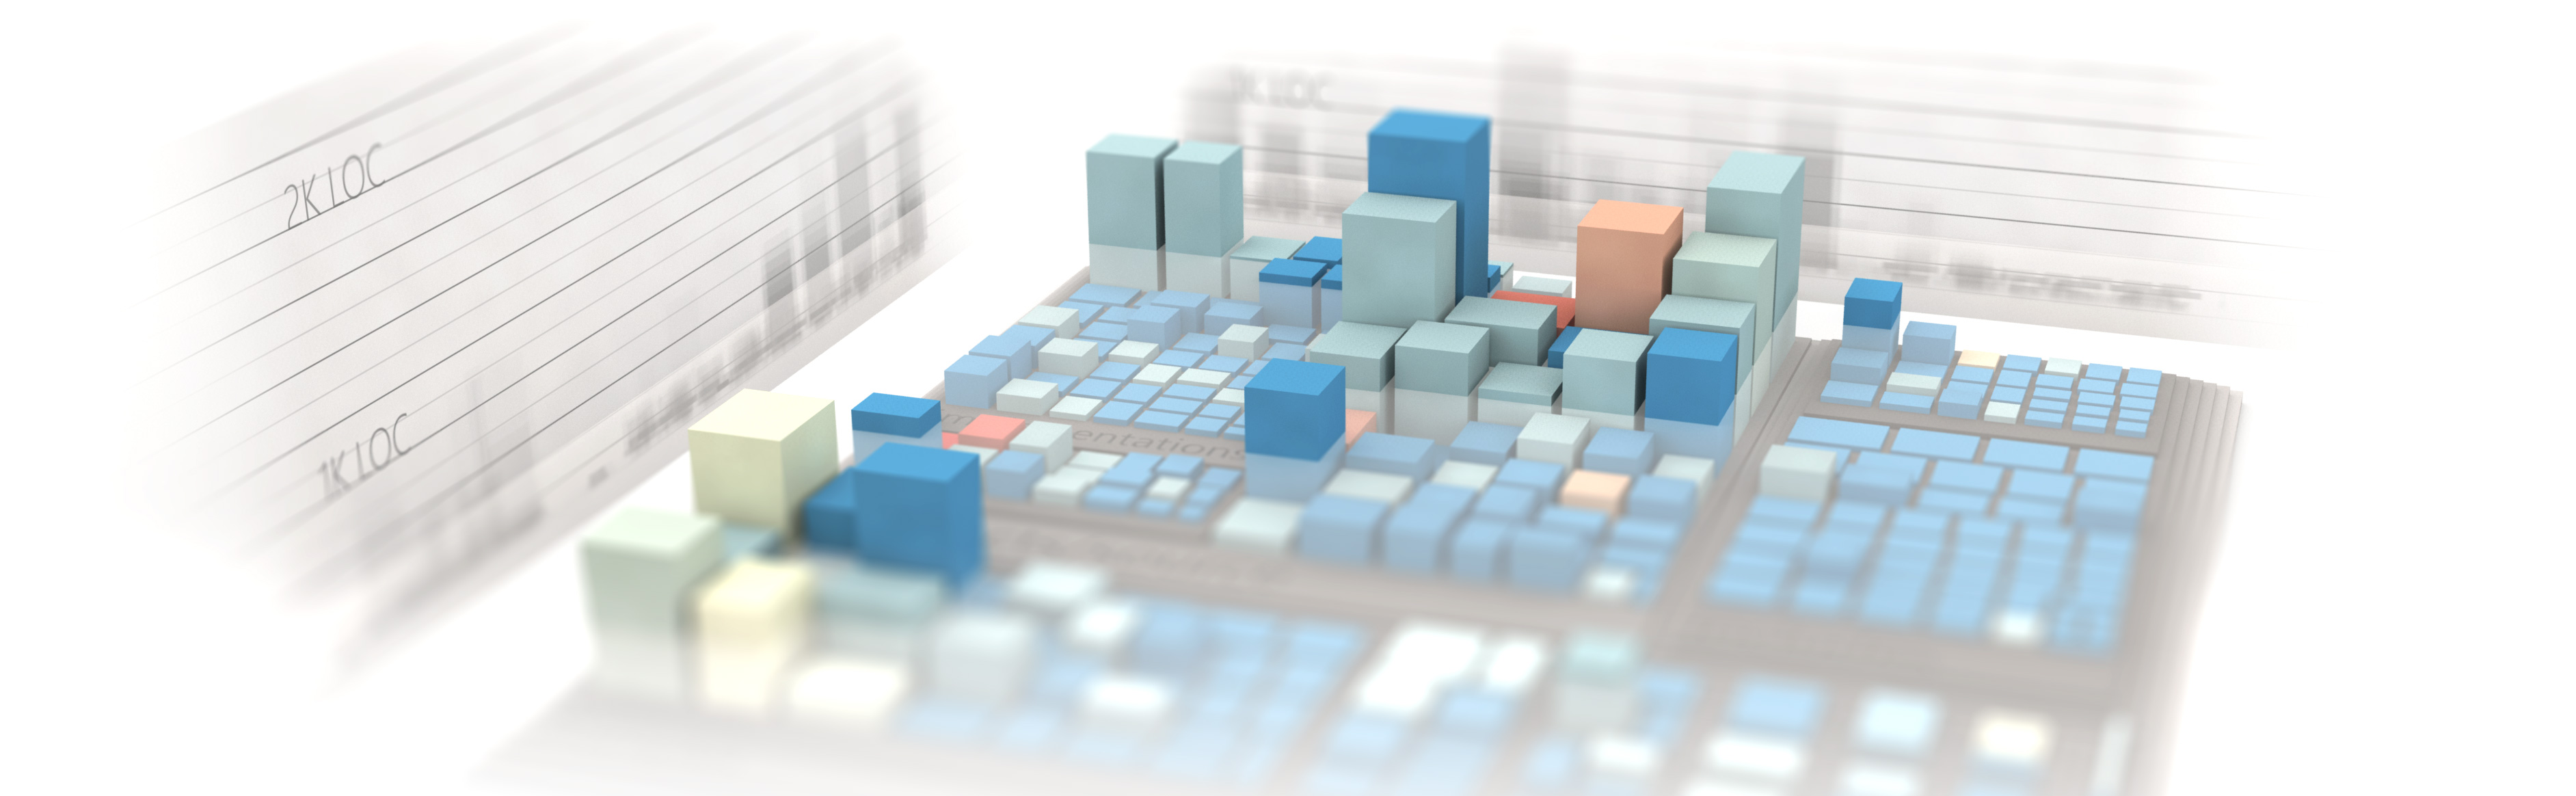
\includegraphics[width=\textwidth]{images/teaser-2.jpg}} 
\author{\underline{Daniel Limberger}, Matthias Trapp, and Jürgen Döllner}
\institute{Hasso Plattner Institute // Faculty of Digital Engineering // University of Potsdam, Germany}

\begin{document} 

\setlength{\leftmargini}{10pt}

\begin{frame}[plain]
	\titlepage
\end{frame} 

\begin{frame}{About this Talk}

    \LARGE
    \blueify{Height Reference}
    \medskip
    
    \normalsize
    Height reference denotes the \blueify{visual display} of an height threshold that can be \blueify{interactively modified} and used for height based queries in \blueify{2.5D treemaps}.
    \bigskip

    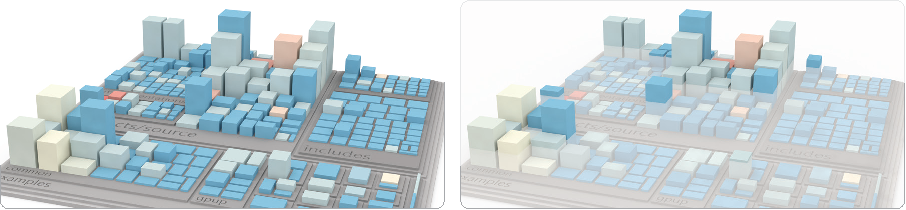
\includegraphics[width=\textwidth]{images/height-reference-teaser} 

\end{frame}

\begin{frame}[t]{Treemaps \enspace}
    
    \bigskip

    \Large
    \blueify{Treemaps \cite{Johnson1991} are used to visualize tree-structured data,}

    \bigskip

    \begin{columns}

        \begin{column}{0.55\textwidth}
            \normalsize
            e.g., stock markets \cite{Wattenberg1999}, \blueify{sensor data} \cite{Mitchell2004}, \blueify{business data} \cite{Vliegen2006}, \blueify{file systems} \cite{Shneiderman1992}, \blueify{software system information} \cite{Wettel2008}.
            
            \bigskip
            \begin{itemize}
                
                \pause
                \item[1.] Non-spatial data is spatialized---it is given a gestalt that preserves the data's structure, e.g., rectangular treemaps use nested rectangles to depict nodes,
                
                \pause
                \item[2.] and data (attributes) are mapped to visual variables, i.e., properties of the rectangles (size and color).
                
            \end{itemize}

        \end{column}   

        \begin{column}{0.38\textwidth}
            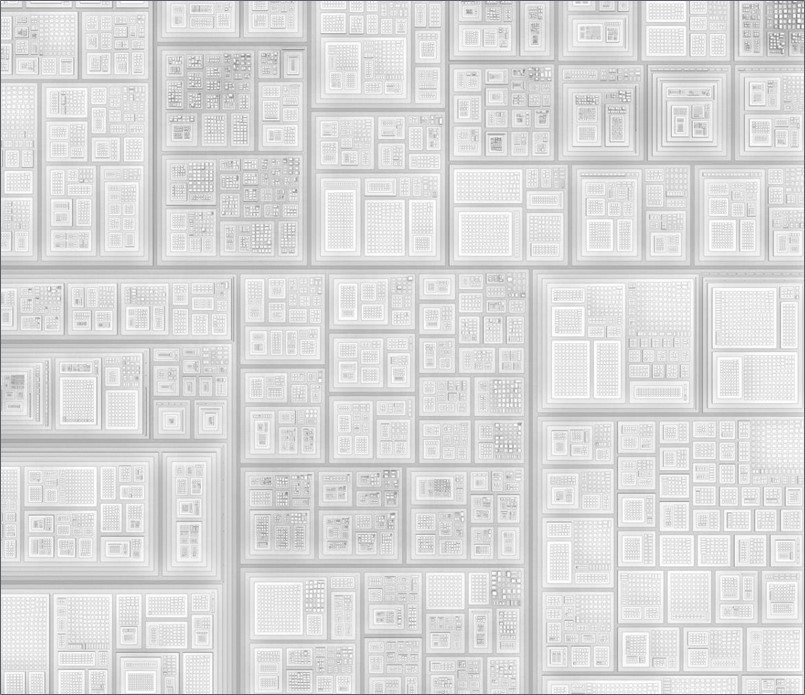
\includegraphics[width=1.8in]{images/flatmap.jpg} 
        \end{column}        

    \end{columns}
        
\end{frame}

\begin{frame}{Treemaps --- Spatialization of Tree-structured Data}
    
    Leaf nodes are colored and have numerical weights, which can represent any associated attribute, e.g., file size.
    The weight of a parent node is defined by the sum of the weights of its child nodes.
    
    \begin{columns}[t]
        \begin{column}{0.47\textwidth}
            
            \centering
            \textcolor{CorporateBlue1}{Simple Graph}
            
        \end{column}   
        
        \begin{column}{0.47\textwidth}
            
            \centering
            \textcolor{CorporateBlue1}{Rectangular Treemap}
            
        \end{column}   
        
    \end{columns}   
    
    \bigskip
    \centering
    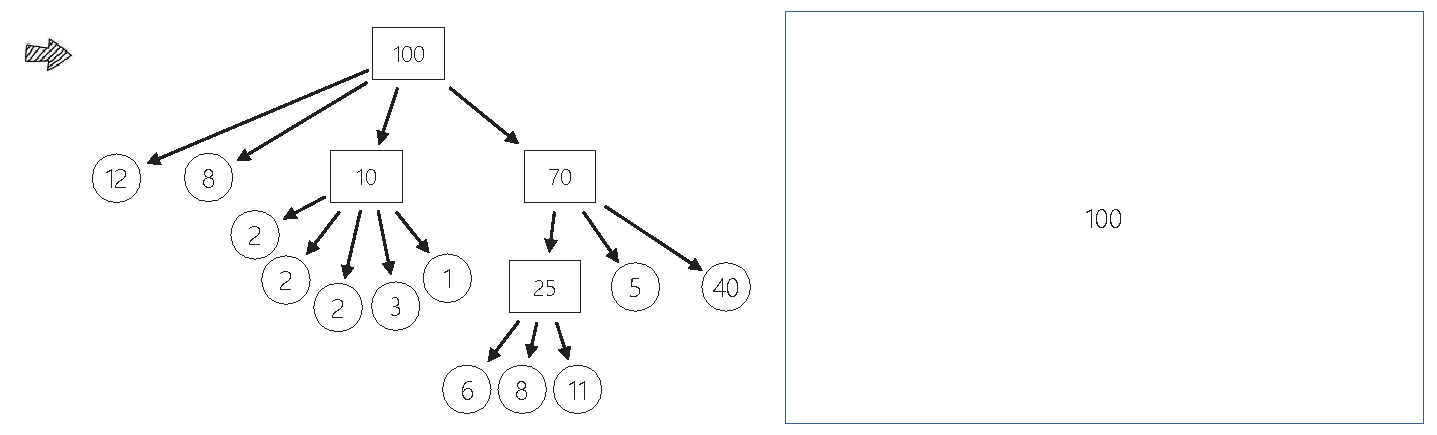
\includegraphics[height=0.475\paperheight]{images/treemap-create-1}
    
\end{frame}

\begin{frame}{Treemaps --- Spatialization of Tree-structured Data}
    
    Leaf nodes are colored and have numerical weights, which can represent any associated attribute, e.g., file size.
    The weight of a parent node is defined by the sum of the weights of its child nodes.
    
    \begin{columns}[t]
        \begin{column}{0.47\textwidth}
            
            \centering
            \textcolor{CorporateBlue1}{Simple Graph}
            
        \end{column}   
        
        \begin{column}{0.47\textwidth}
            
            \centering
            \textcolor{CorporateBlue1}{Rectangular Treemap}
            
        \end{column}   
        
    \end{columns}   
    
    \bigskip
    \centering
    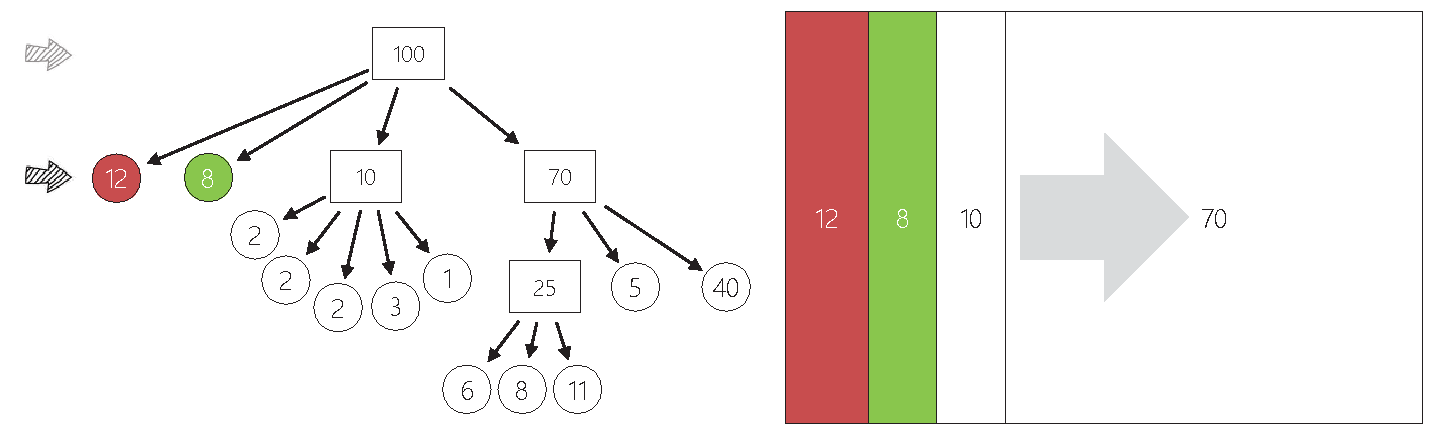
\includegraphics[height=0.475\paperheight]{images/treemap-create-2}
    
\end{frame}

\begin{frame}{Treemaps --- Spatialization of Tree-structured Data}
    
    Leaf nodes are colored and have numerical weights, which can represent any associated attribute, e.g., file size.
    The weight of a parent node is defined by the sum of the weights of its child nodes.
    
    \begin{columns}[t]
        \begin{column}{0.47\textwidth}
            
            \centering
            \textcolor{CorporateBlue1}{Simple Graph}
            
        \end{column}   
        
        \begin{column}{0.47\textwidth}
            
            \centering
            \textcolor{CorporateBlue1}{Rectangular Treemap}
            
        \end{column}   
        
    \end{columns}   
    
    \bigskip
    \centering
    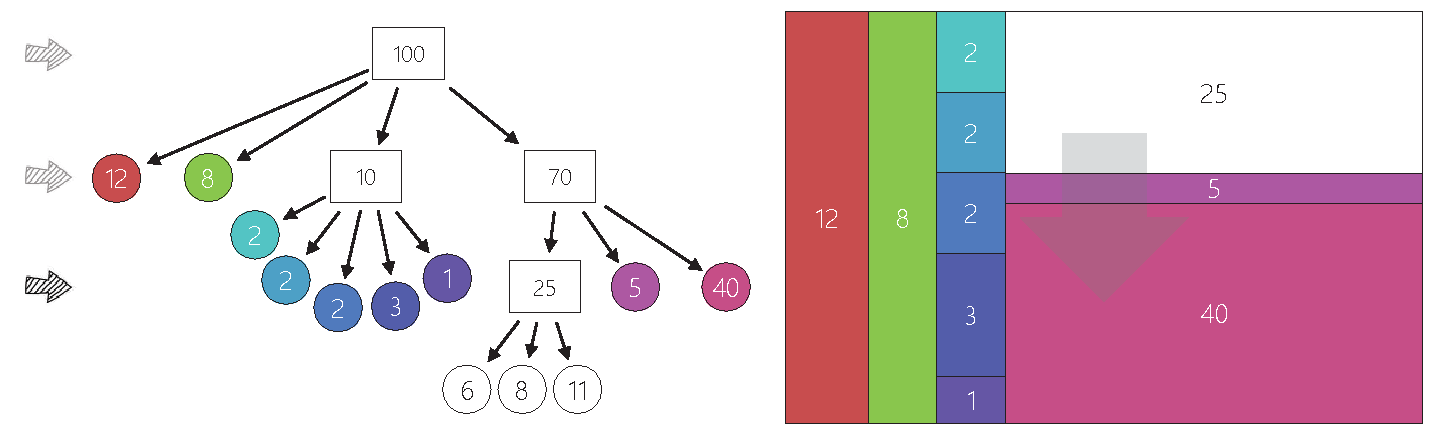
\includegraphics[height=0.475\paperheight]{images/treemap-create-3}
    
\end{frame}

\begin{frame}{Treemaps --- Spatialization of Tree-structured Data}
    
    Leaf nodes are colored and have numerical weights, which can represent any associated attribute, e.g., file size.
    The weight of a parent node is defined by the sum of the weights of its child nodes.
    
    \begin{columns}[t]
        \begin{column}{0.47\textwidth}
            
            \centering
            \textcolor{CorporateBlue1}{Simple Graph}
            
        \end{column}   
        
        \begin{column}{0.47\textwidth}
            
            \centering
            \textcolor{CorporateBlue1}{Rectangular Treemap}
            
        \end{column}   
        
    \end{columns}   
    
    \bigskip
    \centering
    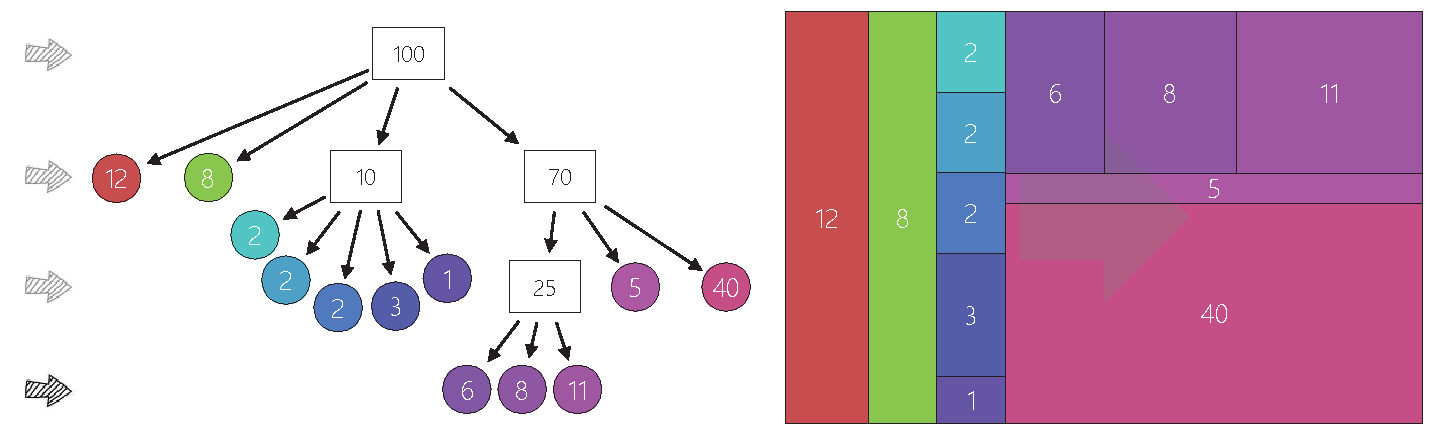
\includegraphics[height=0.475\paperheight]{images/treemap-create-4}
    
\end{frame}

\begin{frame}{Treemaps --- Spatialization of Tree-structured Data}
    
    Leaf nodes are colored and have numerical weights, which can represent any associated attribute, e.g., file size.
    The weight of a parent node is defined by the sum of the weights of its child nodes.
    
    \begin{columns}[t]
        \begin{column}{0.47\textwidth}
            
            \centering
            \textcolor{CorporateBlue1}{Simple Graph}
            
        \end{column}   
        
        \begin{column}{0.47\textwidth}
            
            \centering
            \textcolor{CorporateBlue1}{Rectangular Treemap}
            
        \end{column}   
        
    \end{columns}   
    
    \bigskip
    \centering
    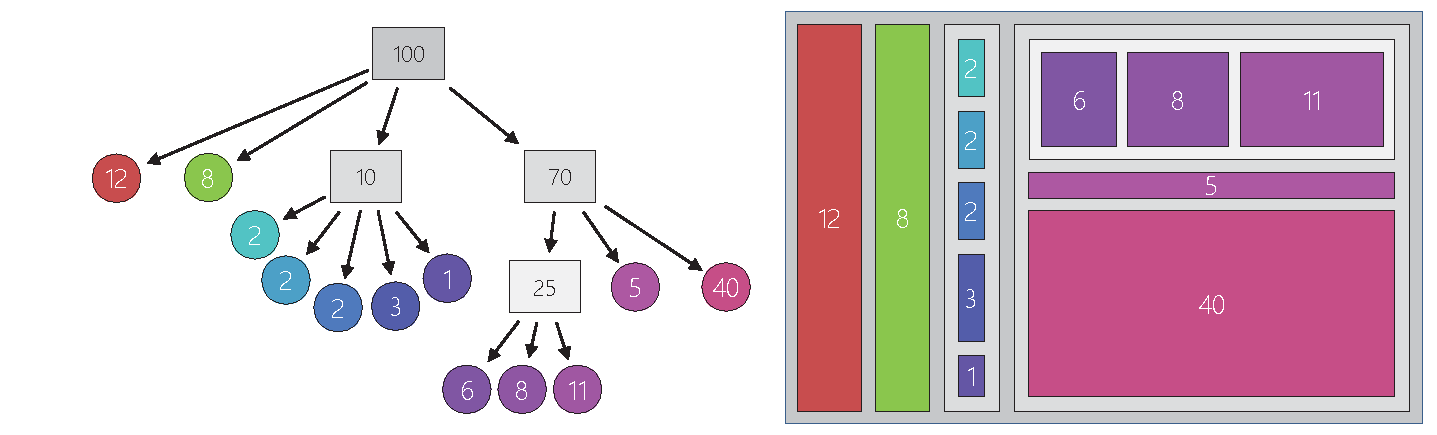
\includegraphics[height=0.475\paperheight]{images/treemap-create-5}
    
\end{frame}

{
\usebackgroundtemplate{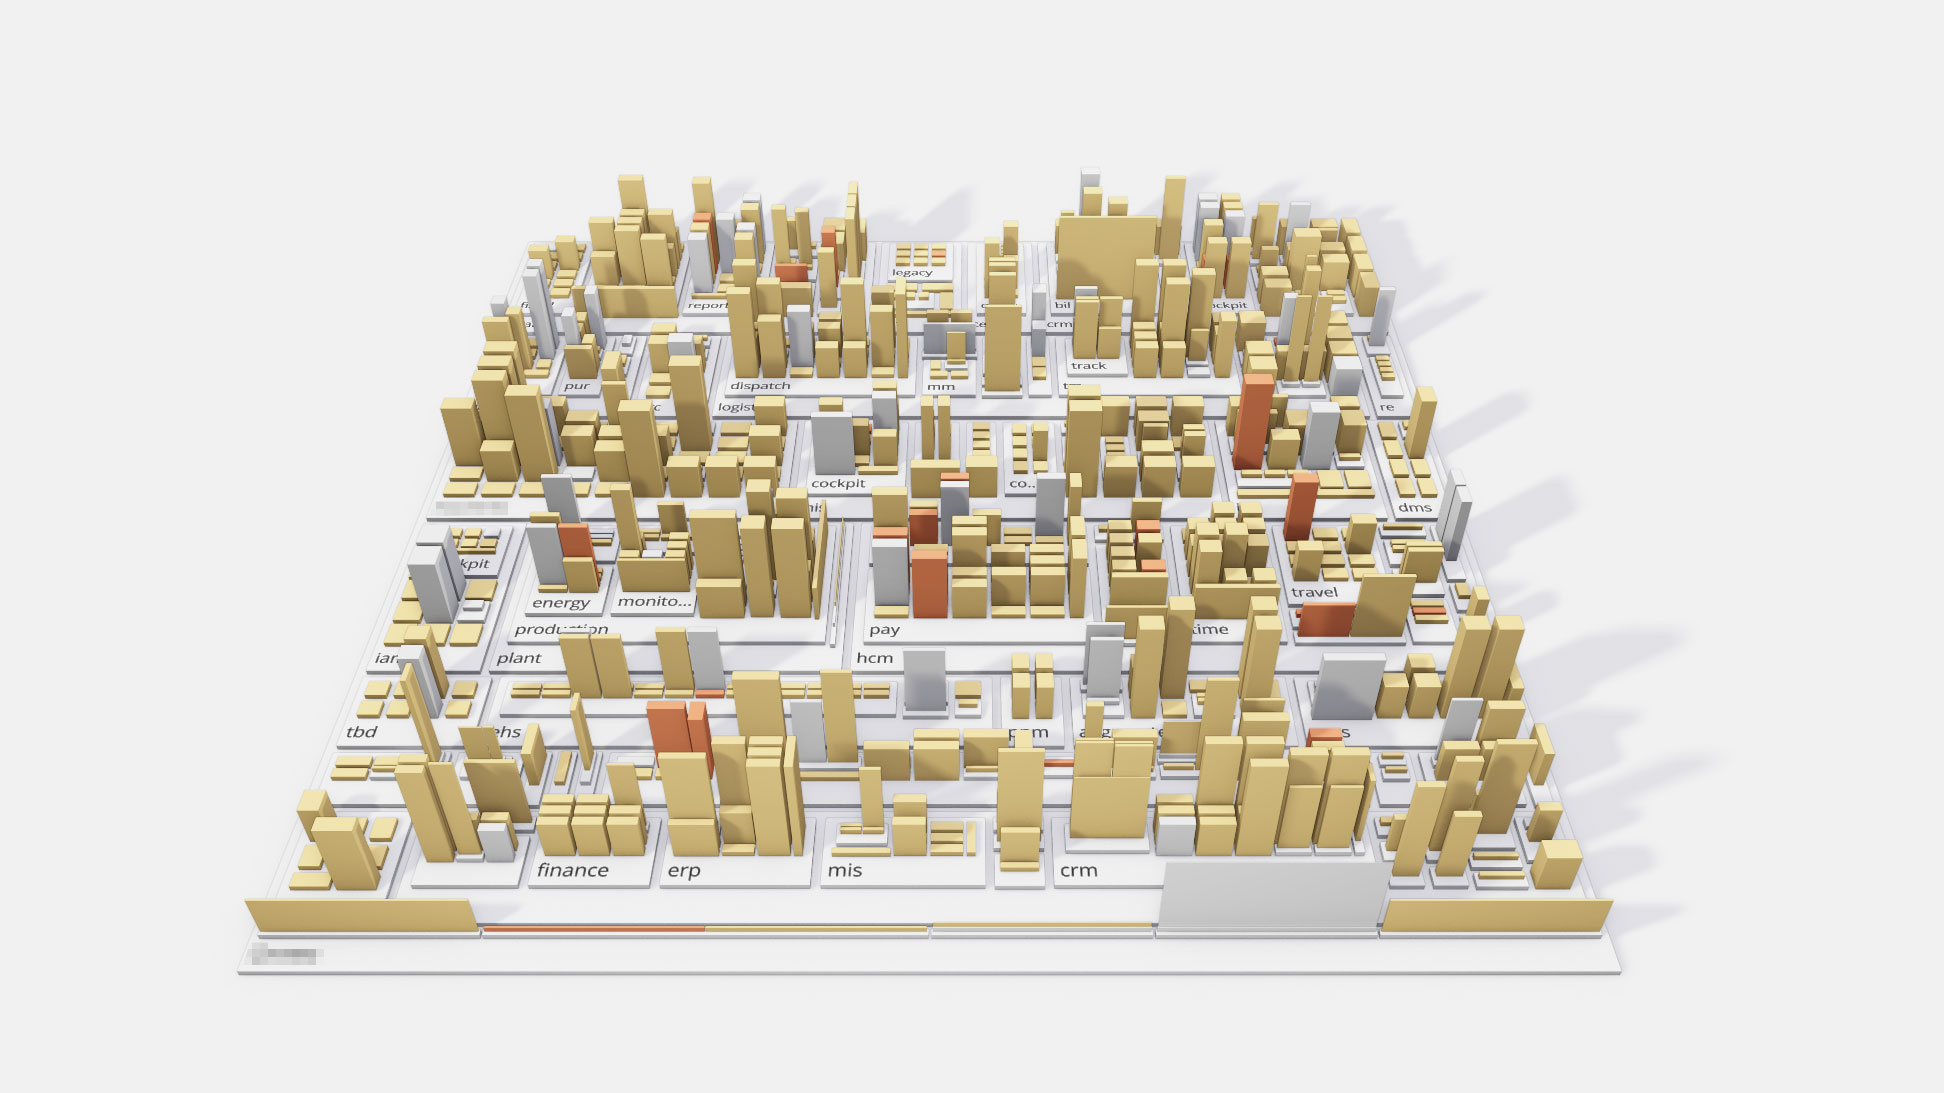
\includegraphics[height=\paperheight]{images/cemex-painter}}

\begin{frame}[t]{Treemaps --- Adding Height as Visual Variable}
    
    \bigskip
    \bigskip
    2.5D Treemap \cite{Bladh2004}
    
\end{frame}
}

{
\usebackgroundtemplate{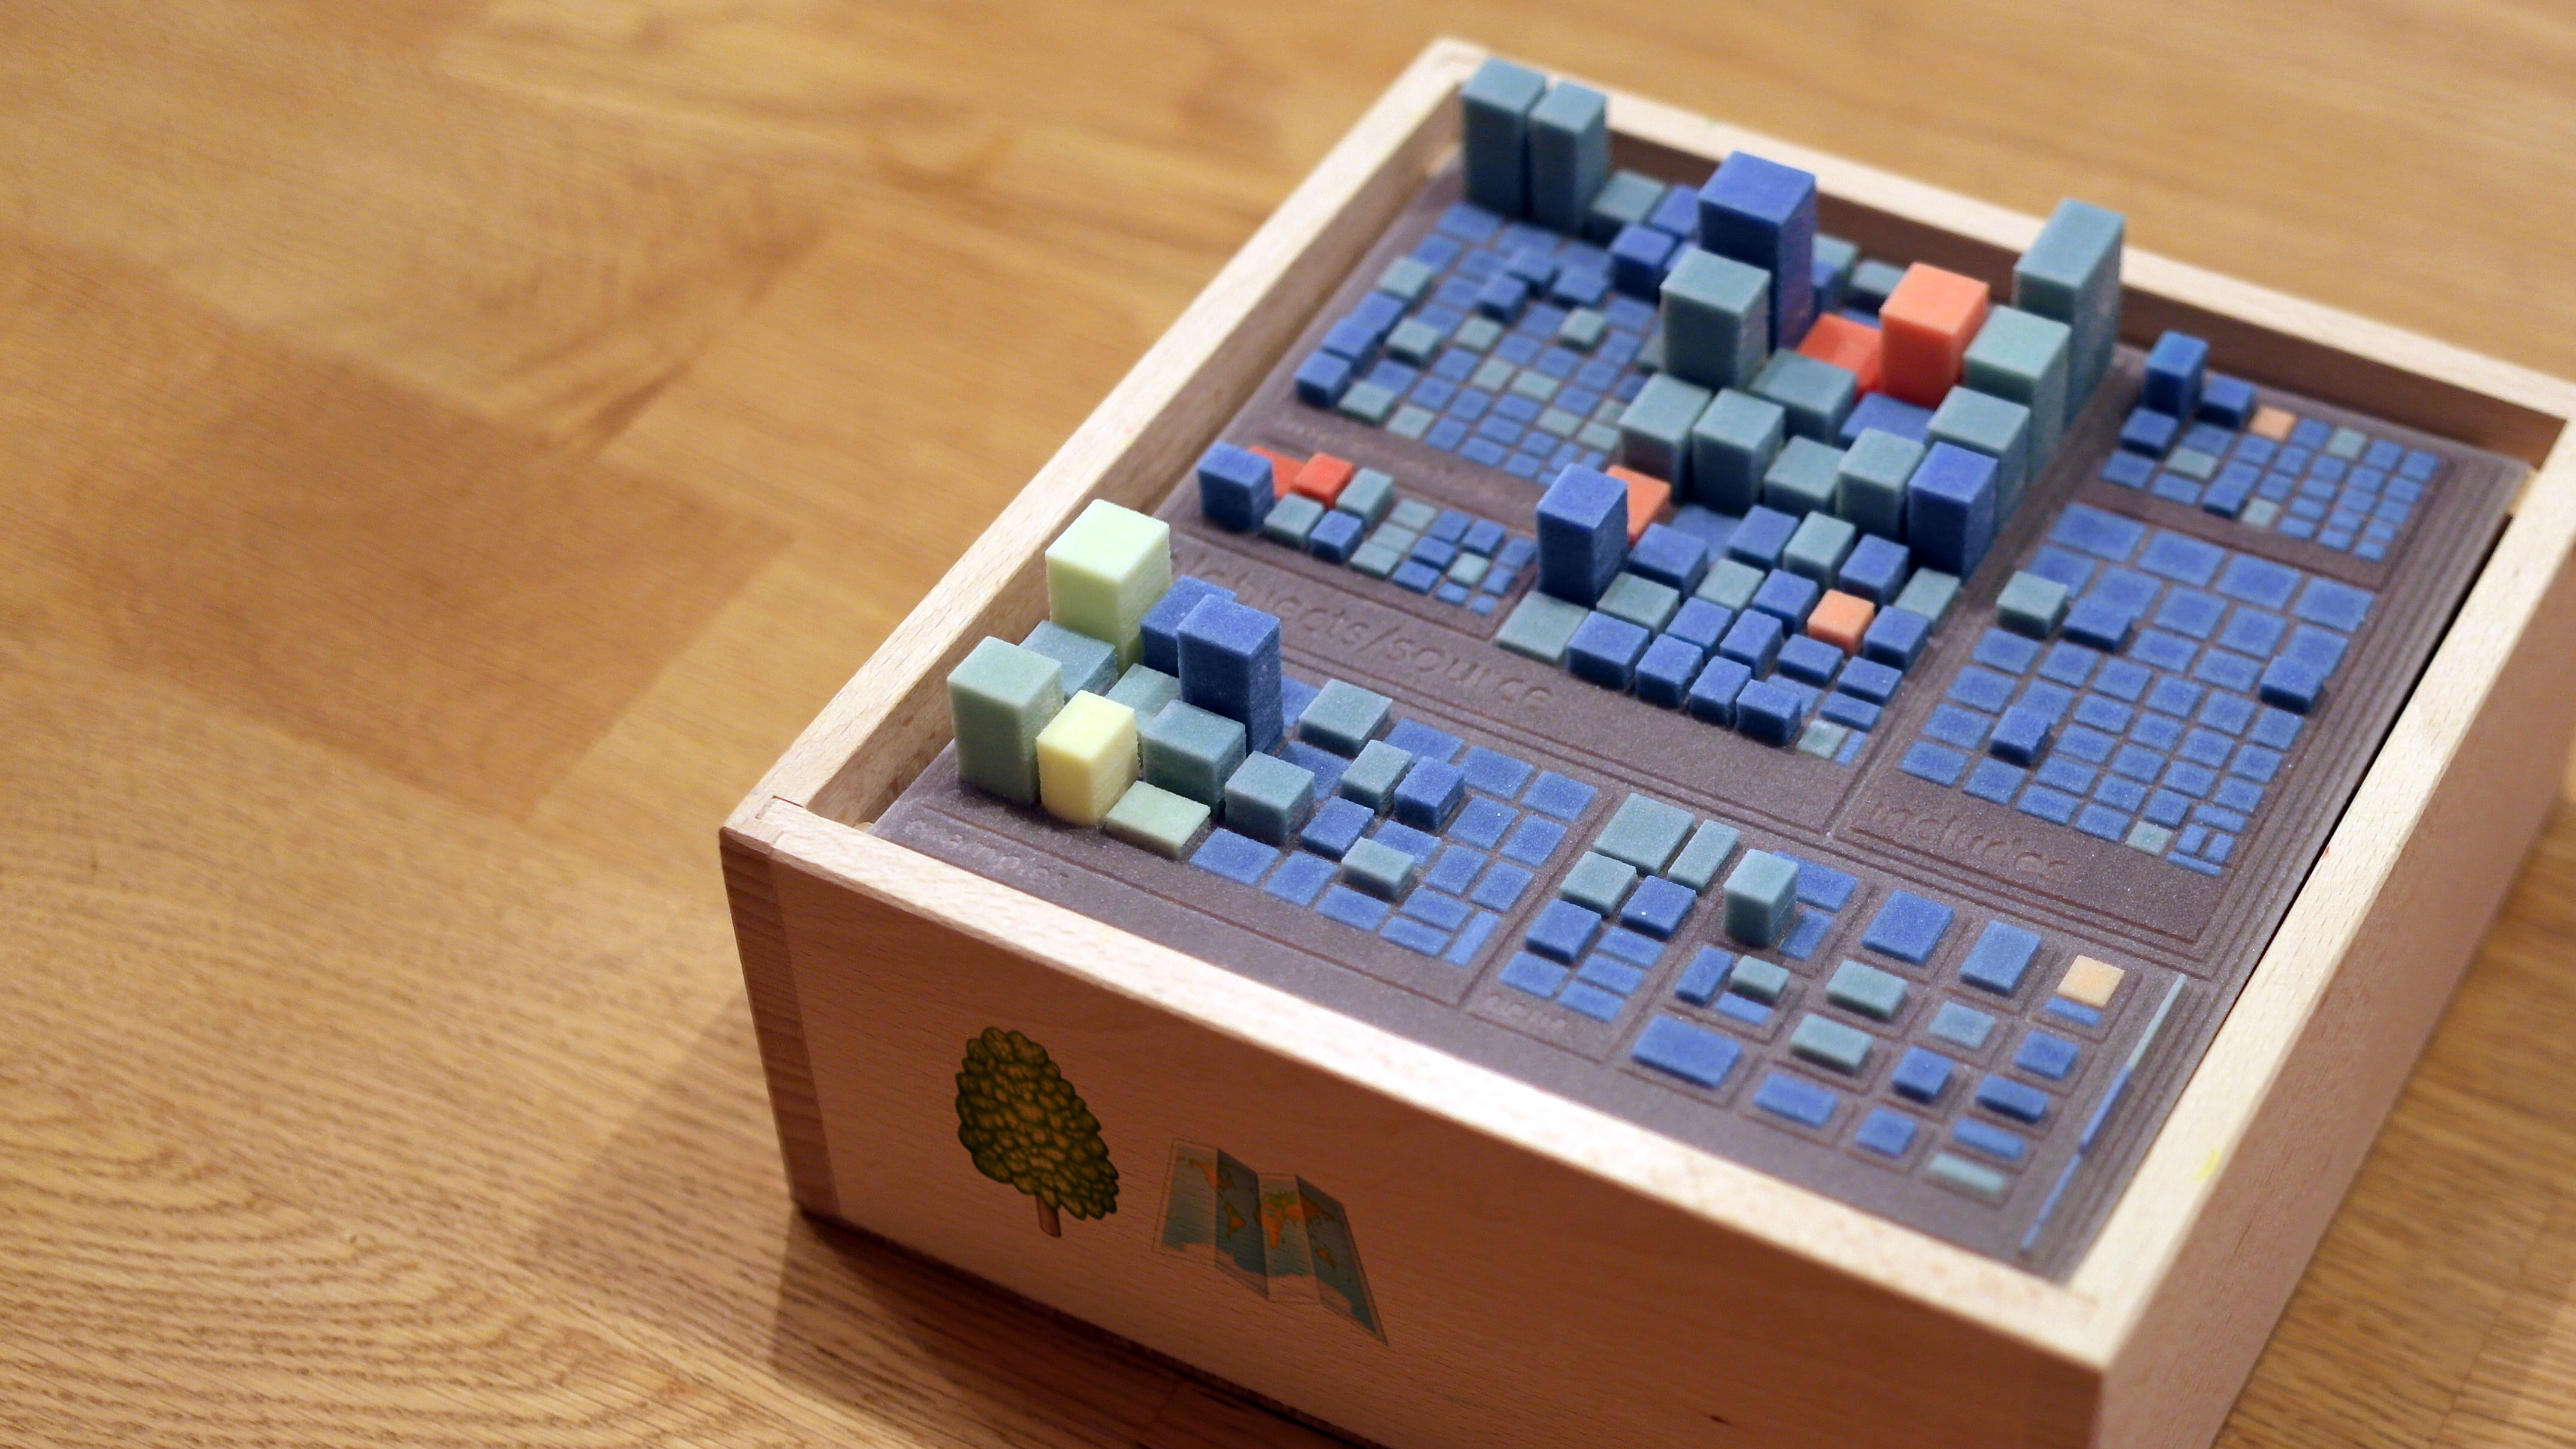
\includegraphics[height=\paperheight]{images/softwaremap-real}}

\begin{frame}{Software Maps --- Basic Example}

    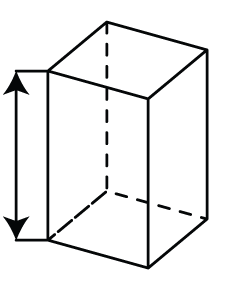
\includegraphics[width=0.35in]{images/visual-variables-height} 
    
    \normalsize\textbf{\# complexity}
    
    \small nesting-level or McCabe
    \bigskip

    
\includegraphics[width=0.35in]{images/visual-variables-color} 
    
    \normalsize\textbf{\# developers}
    
    \small that touched this unit
    \bigskip

    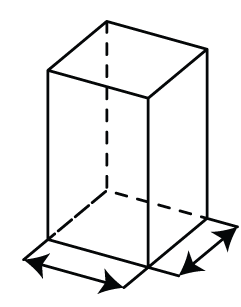
\includegraphics[width=0.35in]{images/visual-variables-footprint} 
    
    \normalsize\textbf{\# lines-of-code}

\end{frame}
} 

\begin{frame}[c]{Research Motivation}

    \centering \Large
    Make 2.5D treemaps a more expressive and interactive communication artifact by increasing its \blueify{provisioning} and overall \blueify{performance}. 

\end{frame}

{
\usebackgroundtemplate{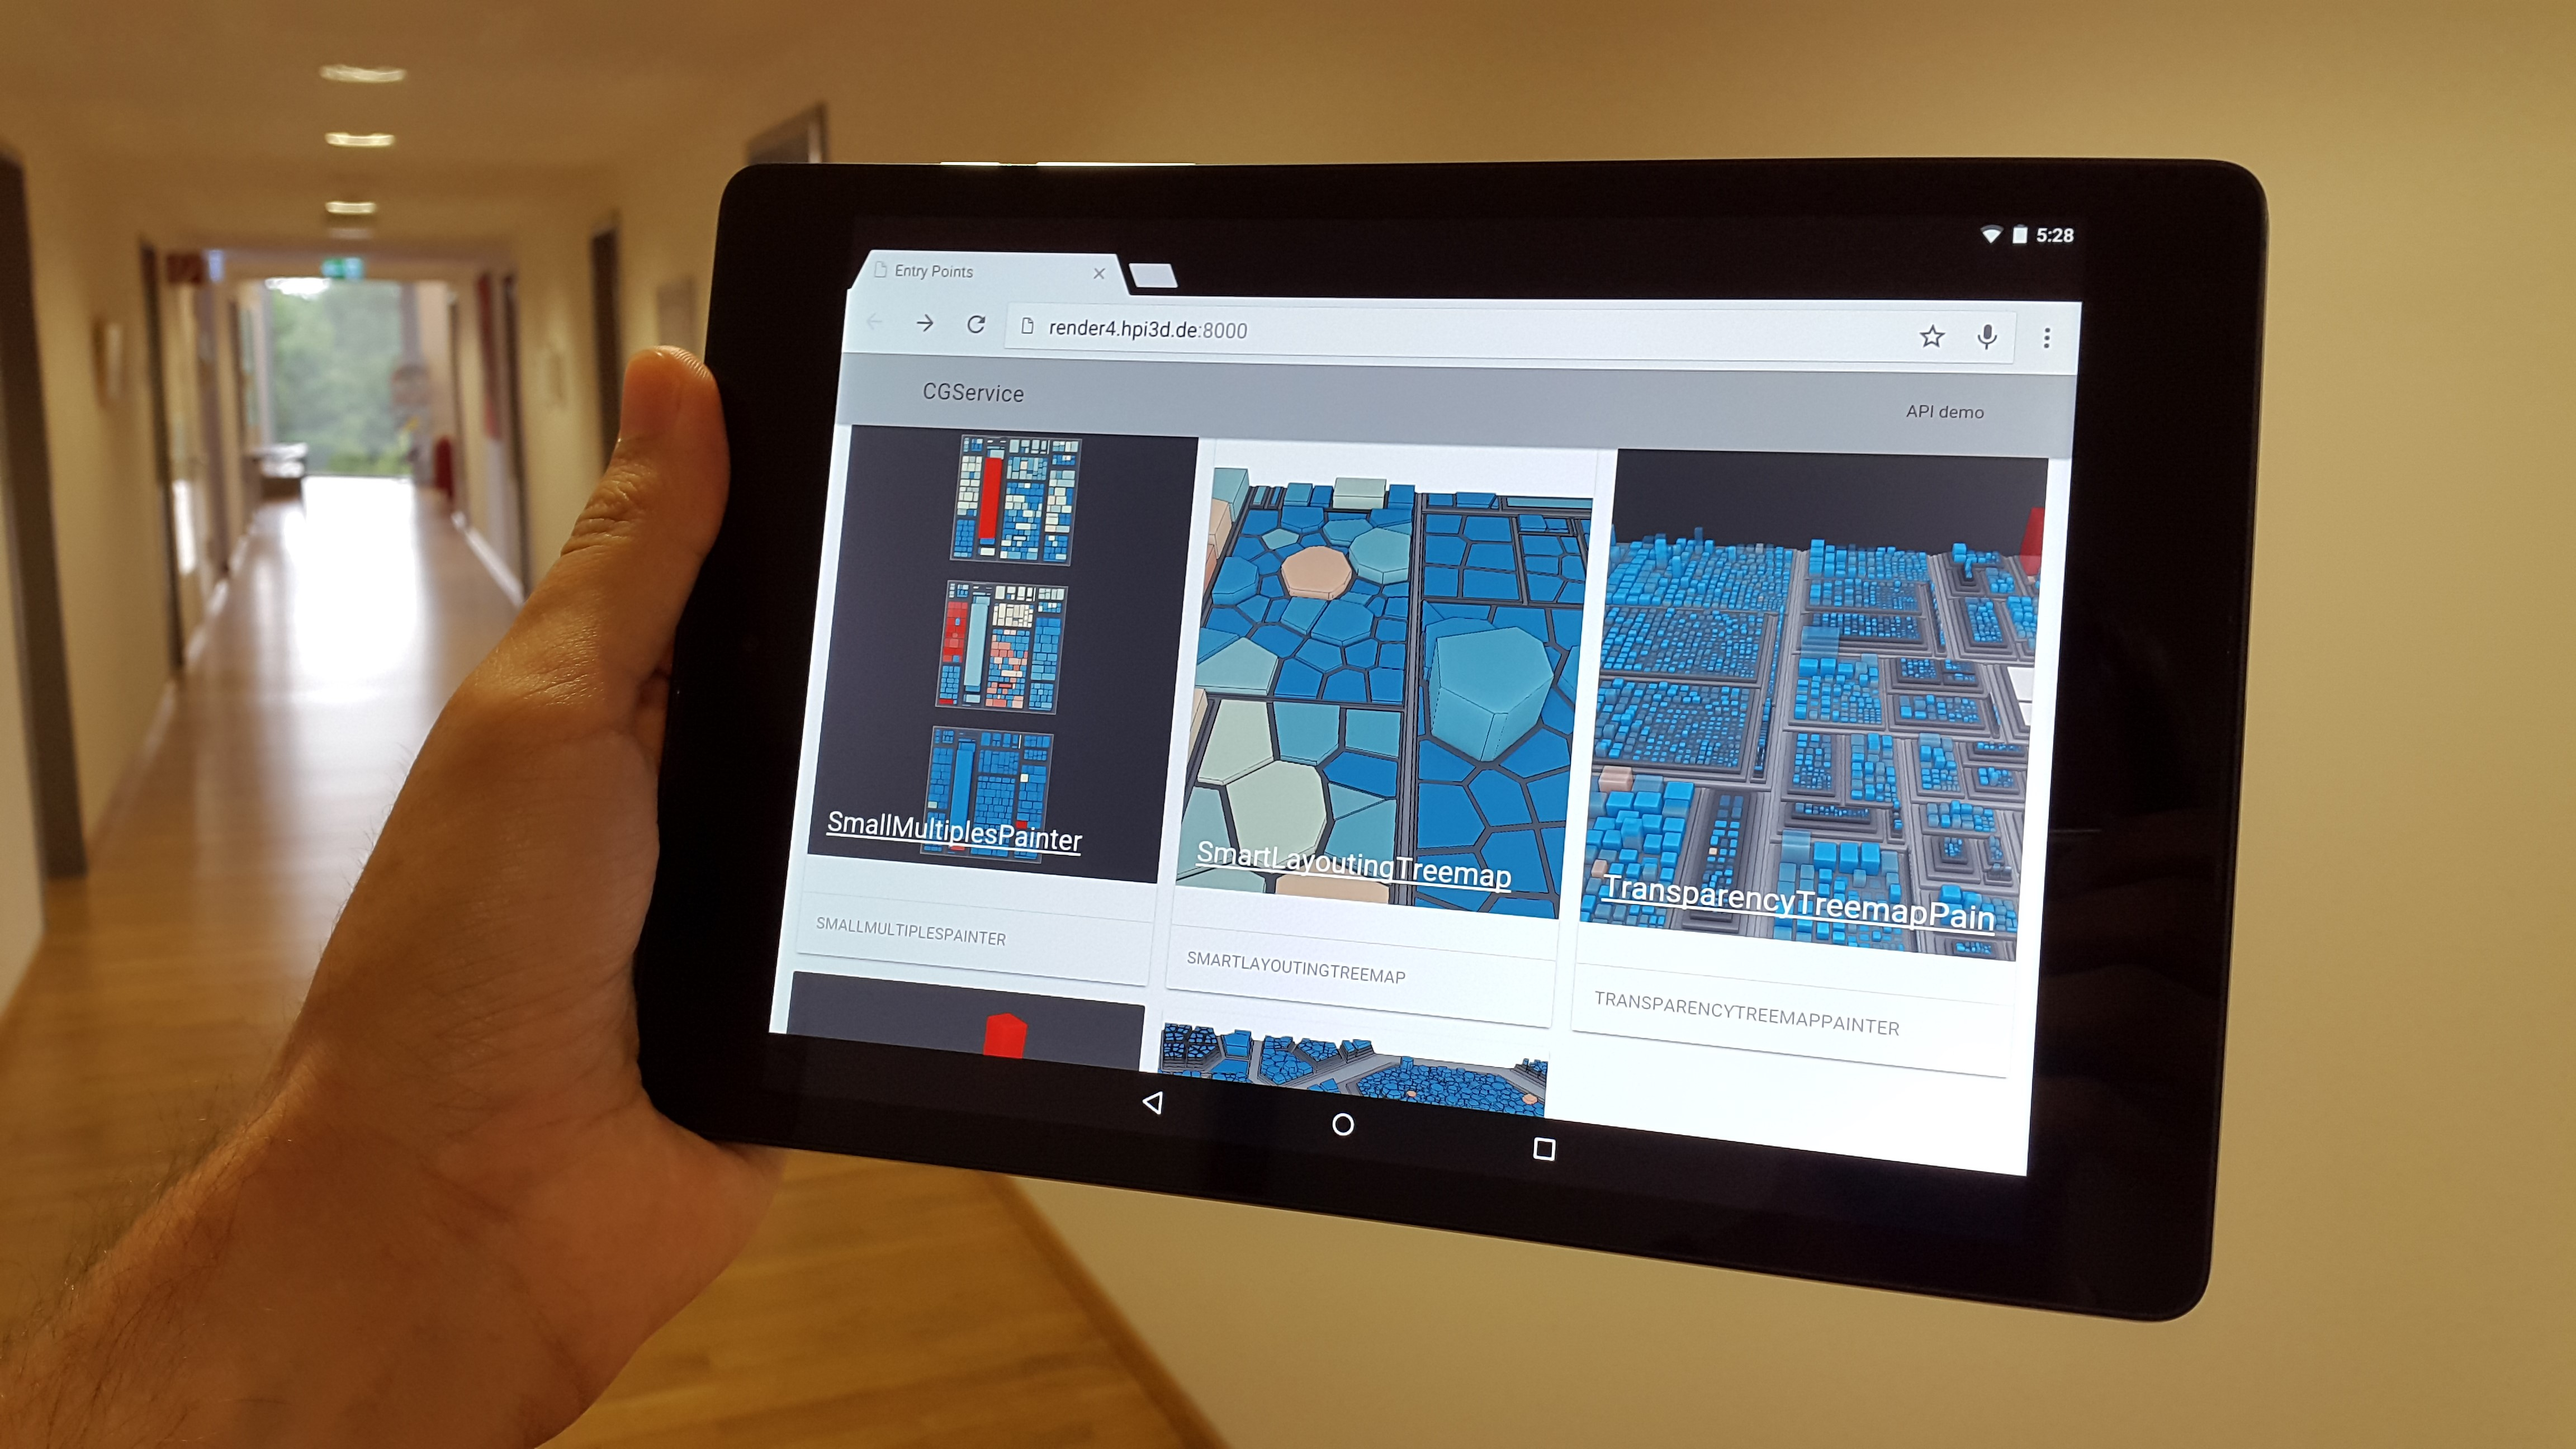
\includegraphics[height=\paperheight]{images/showcase/mobile-provisioning}}
\begin{frame}{~}
\end{frame}
}

{
\usebackgroundtemplate{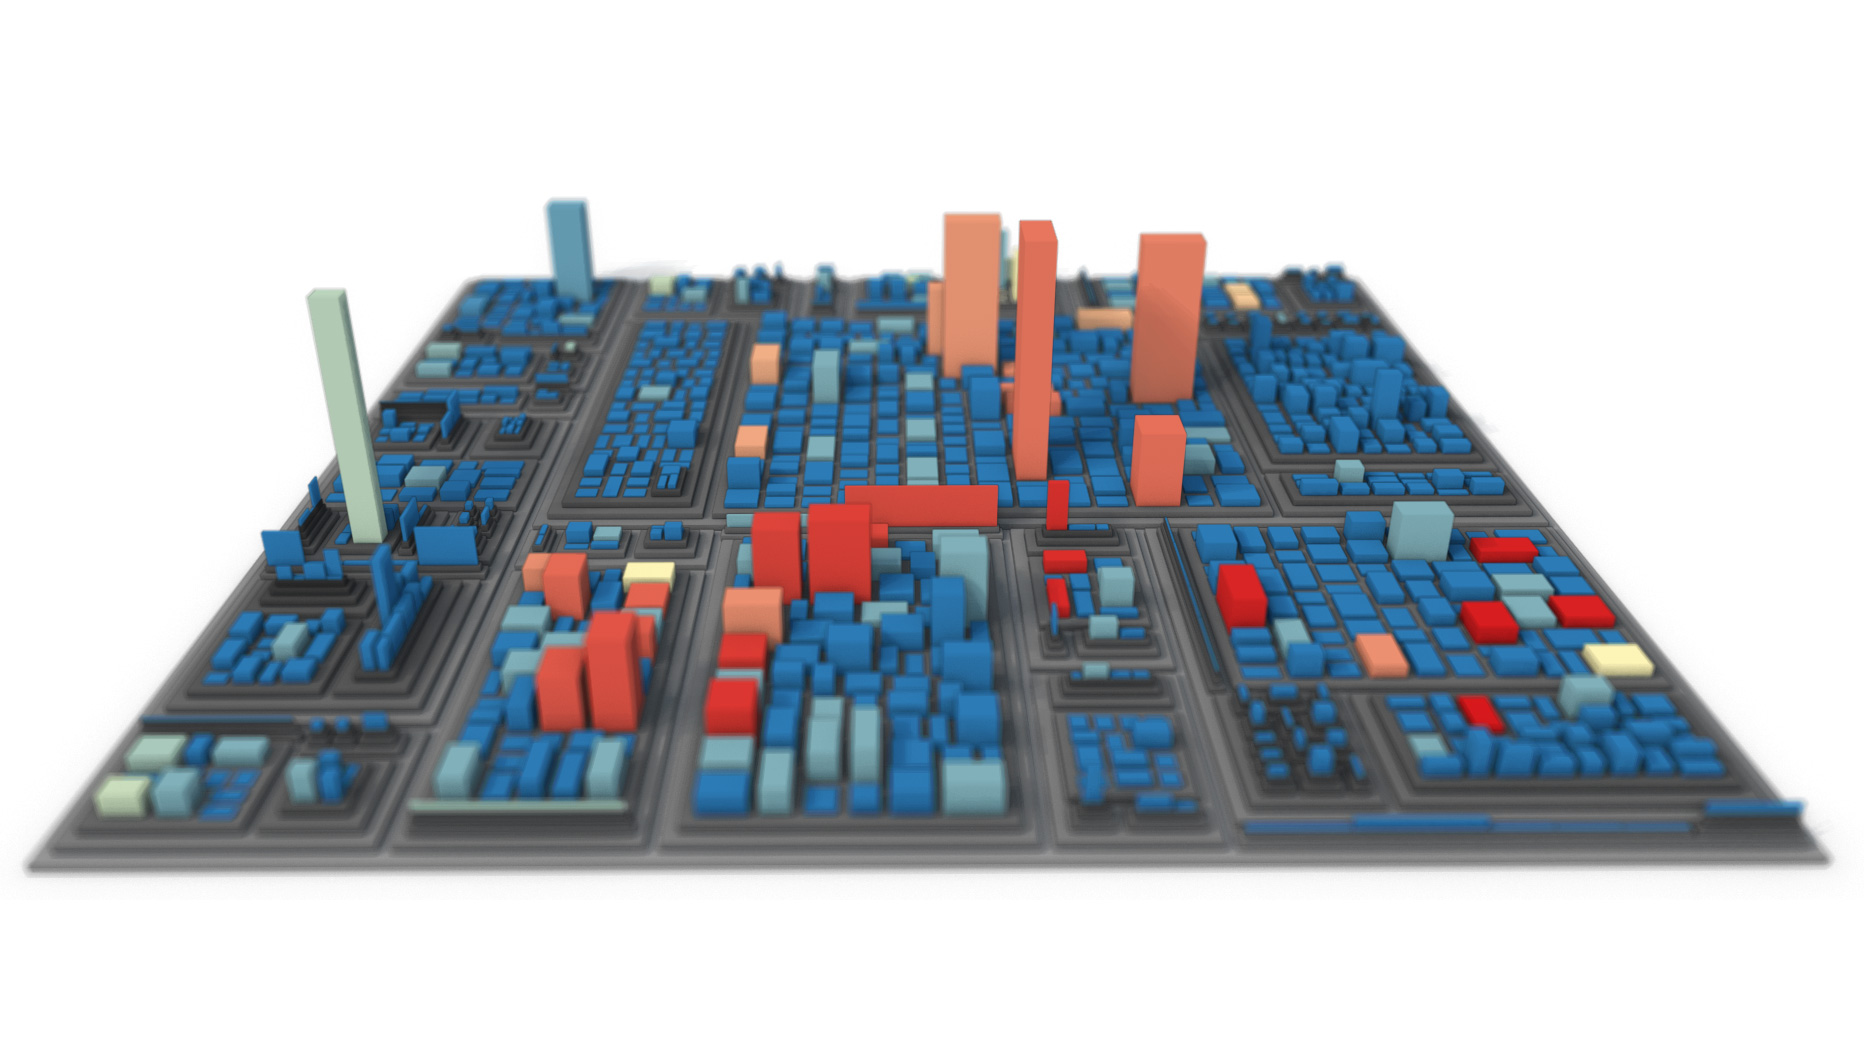
\includegraphics[height=\paperheight]{images/showcase/mobile-multiframe}}
\begin{frame}{~}
\end{frame}
}

{
\usebackgroundtemplate{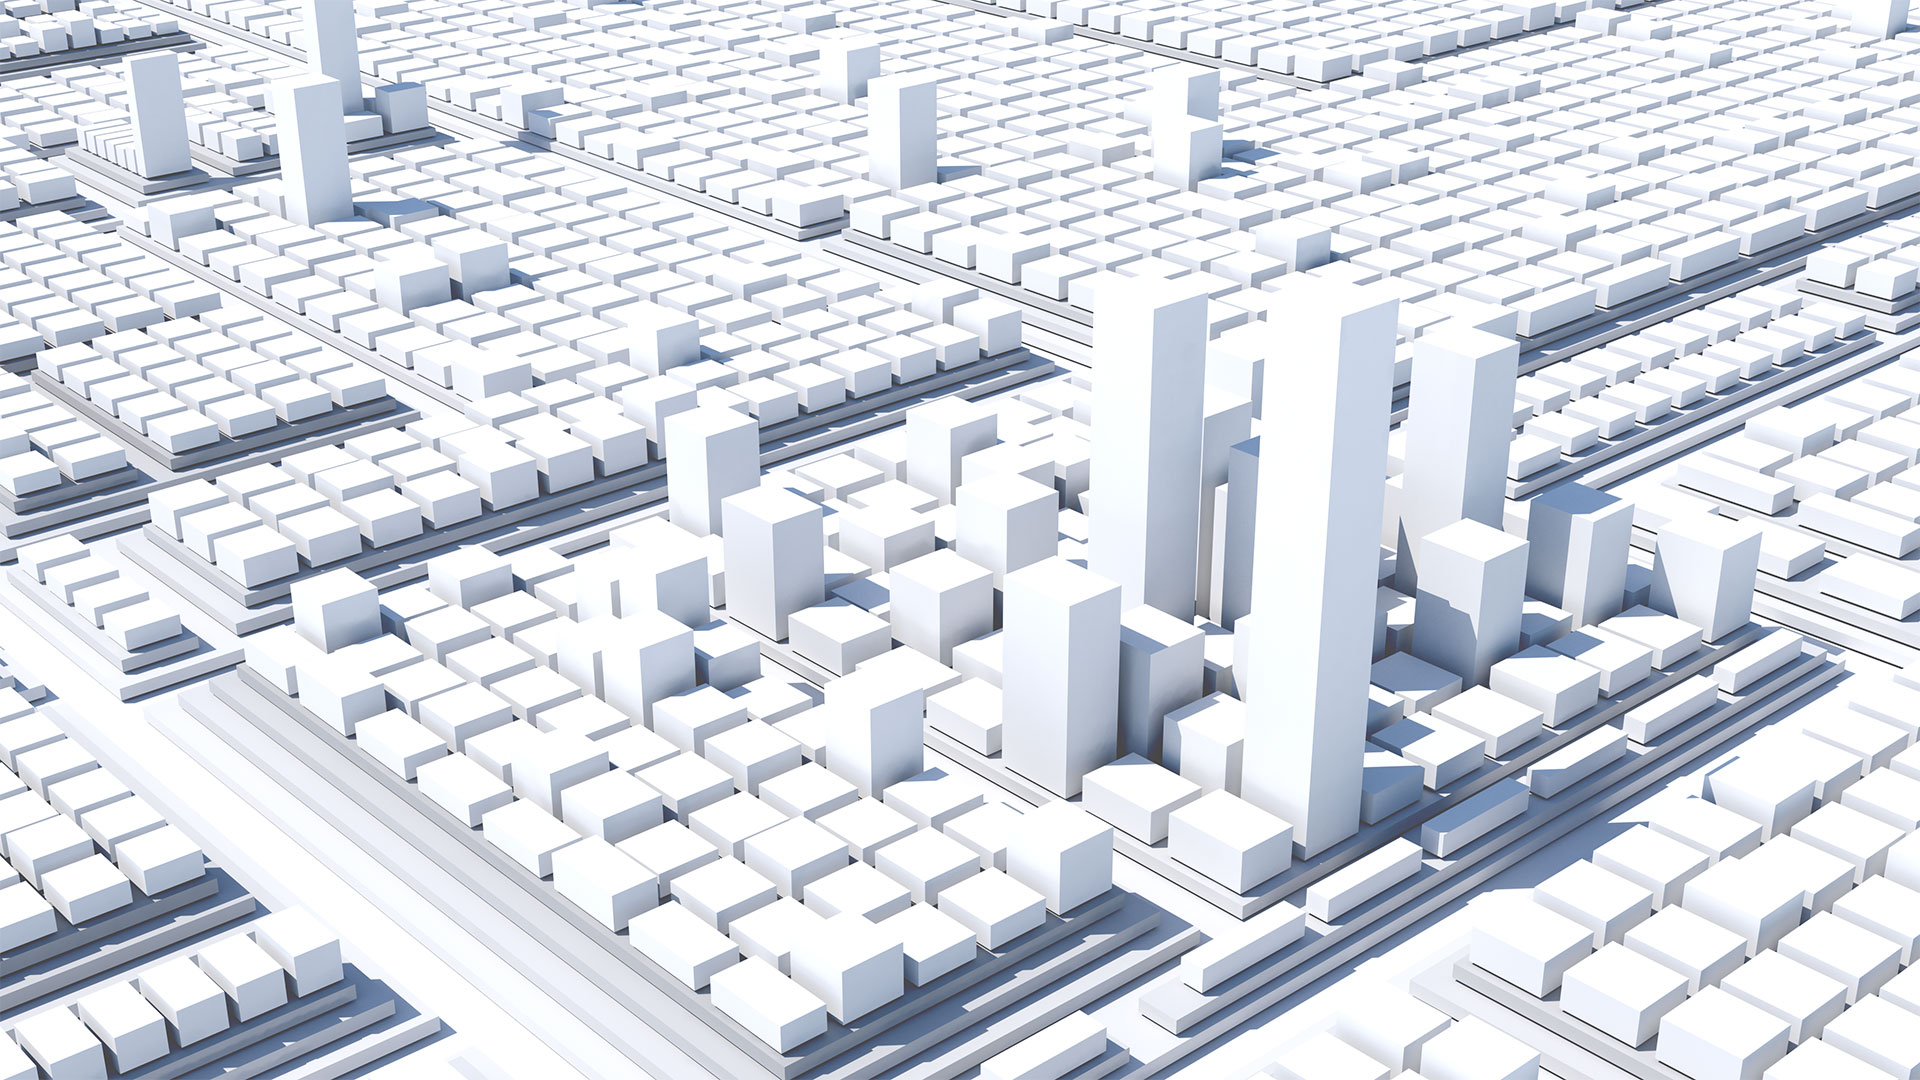
\includegraphics[height=\paperheight]{images/showcase/whitecity}}
\begin{frame}{~}
\end{frame}
}

{
\usebackgroundtemplate{
\includegraphics[height=\paperheight]{images/showcase/whitecity-colored}}
\begin{frame}{~}
\end{frame}
}

{
\usebackgroundtemplate{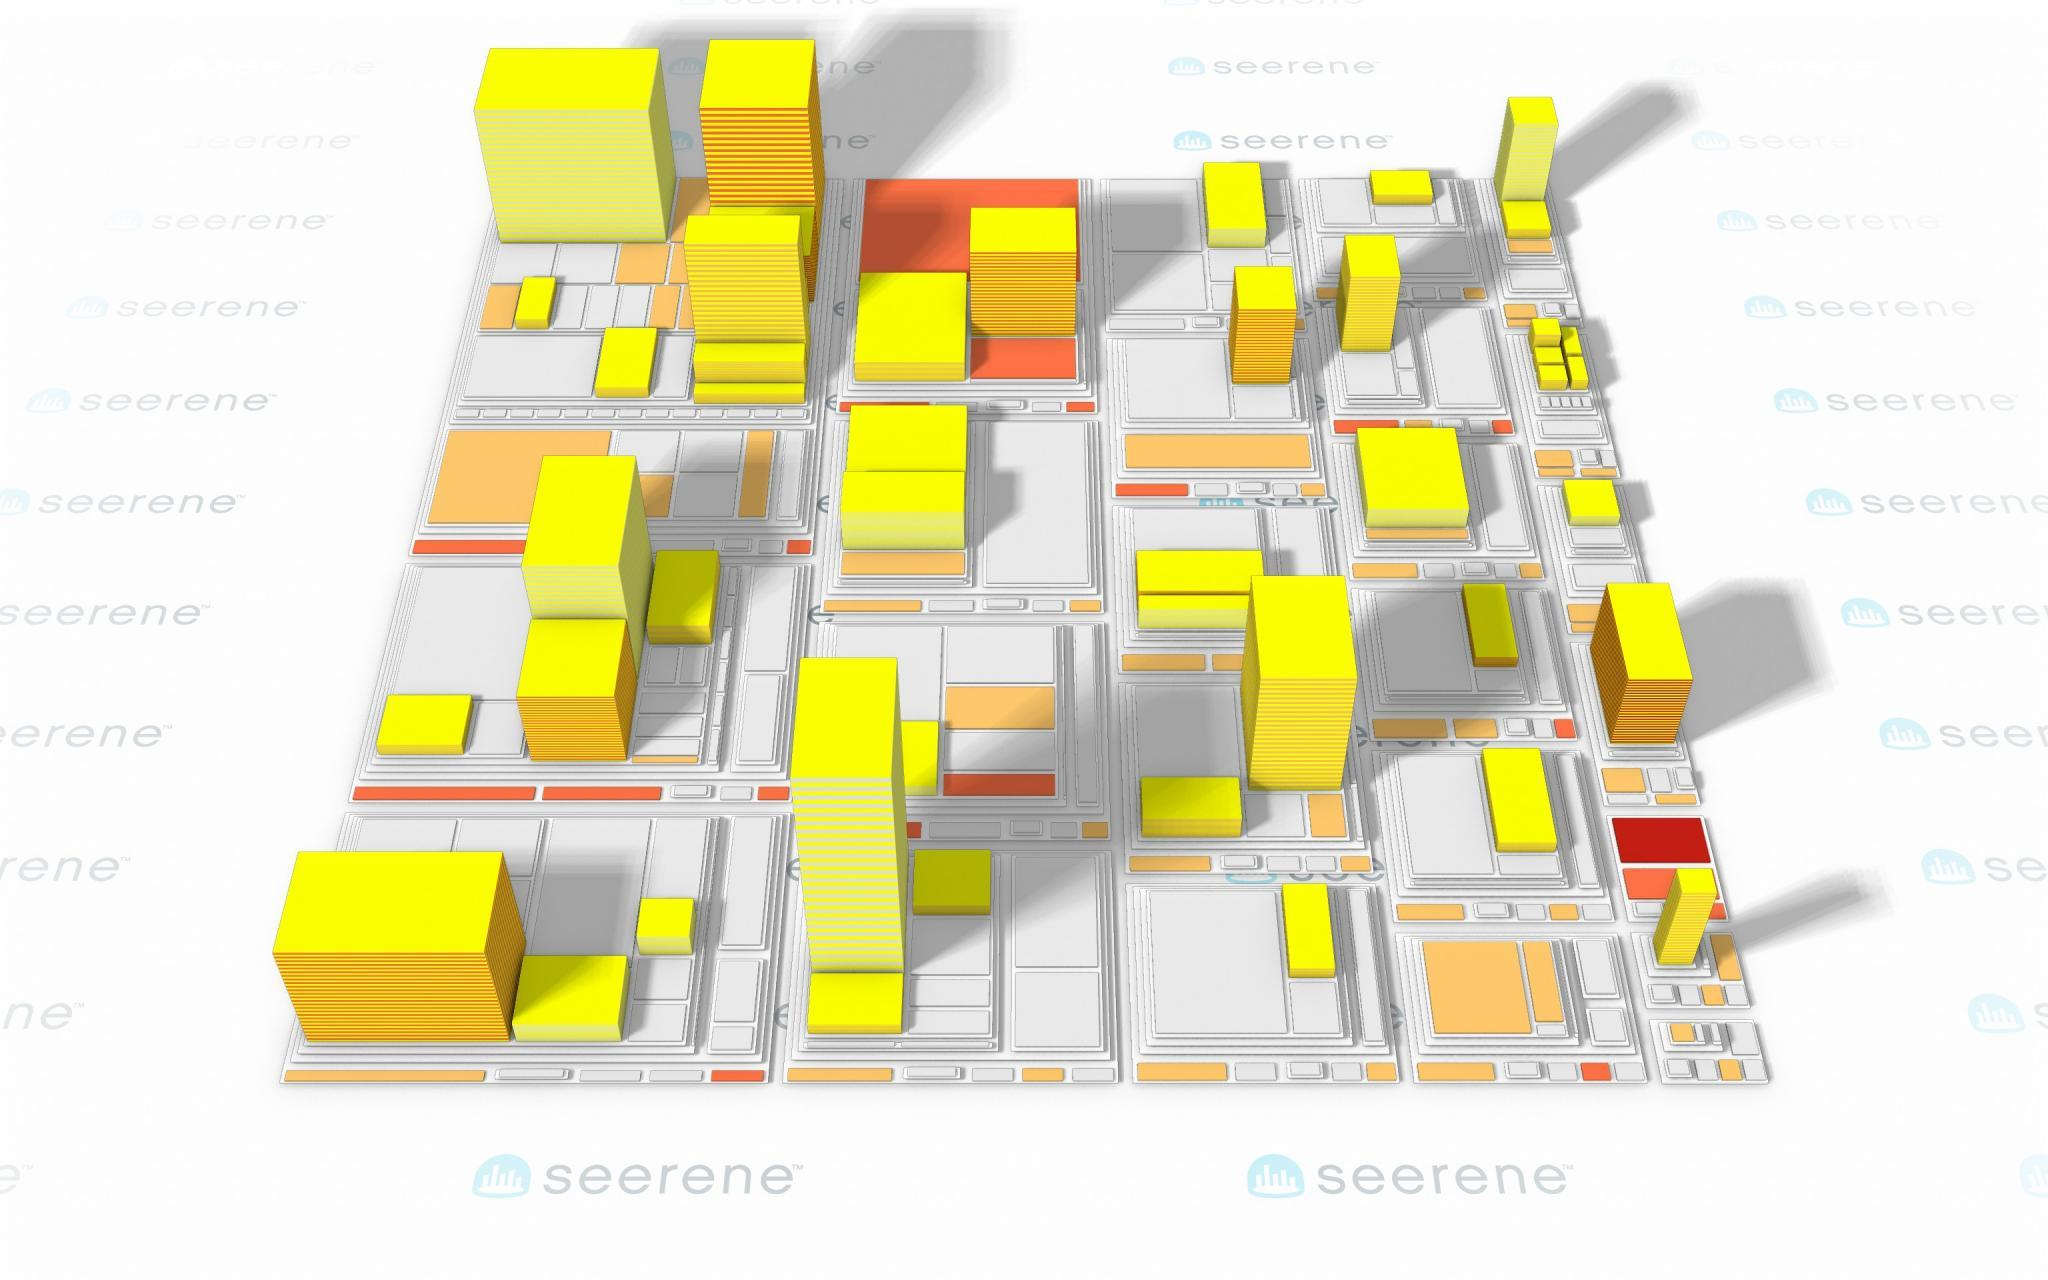
\includegraphics[height=\paperheight]{images/showcase/procedural-texturing}}
\begin{frame}{~}
\end{frame}
}

{
\usebackgroundtemplate{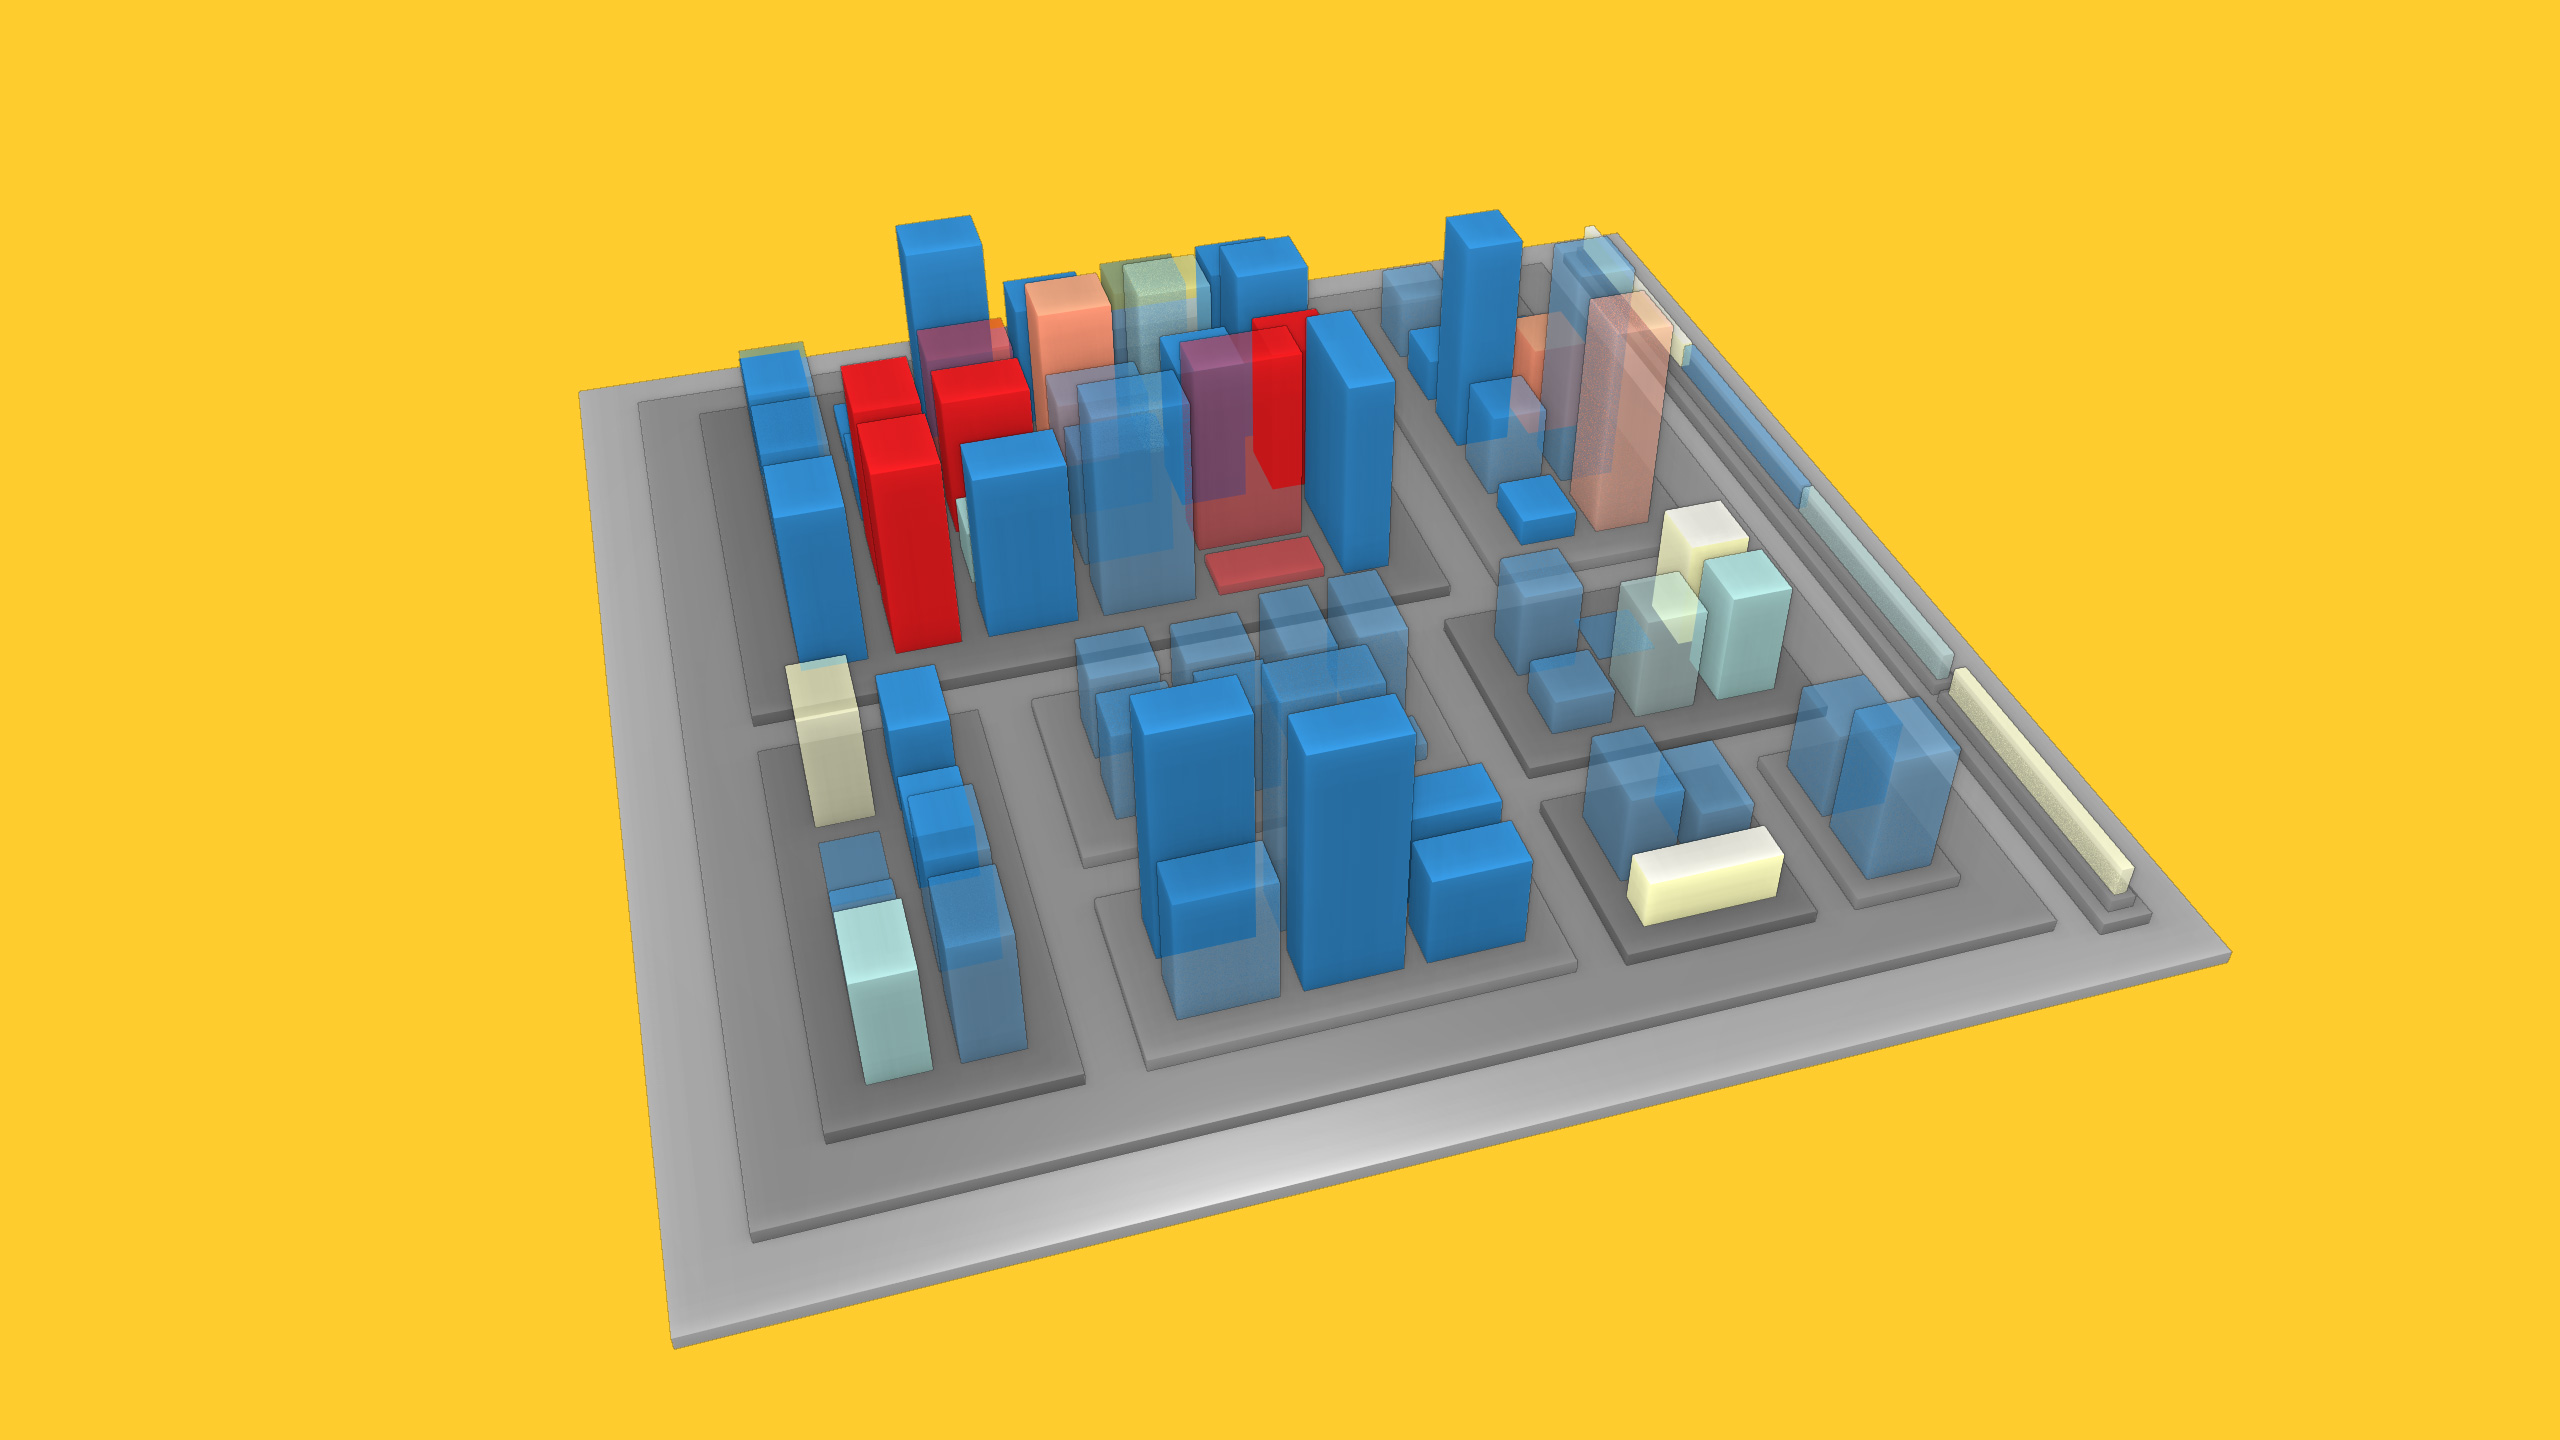
\includegraphics[height=\paperheight]{images/showcase/transparency}}
\begin{frame}{~}
\end{frame}
}

{
\usebackgroundtemplate{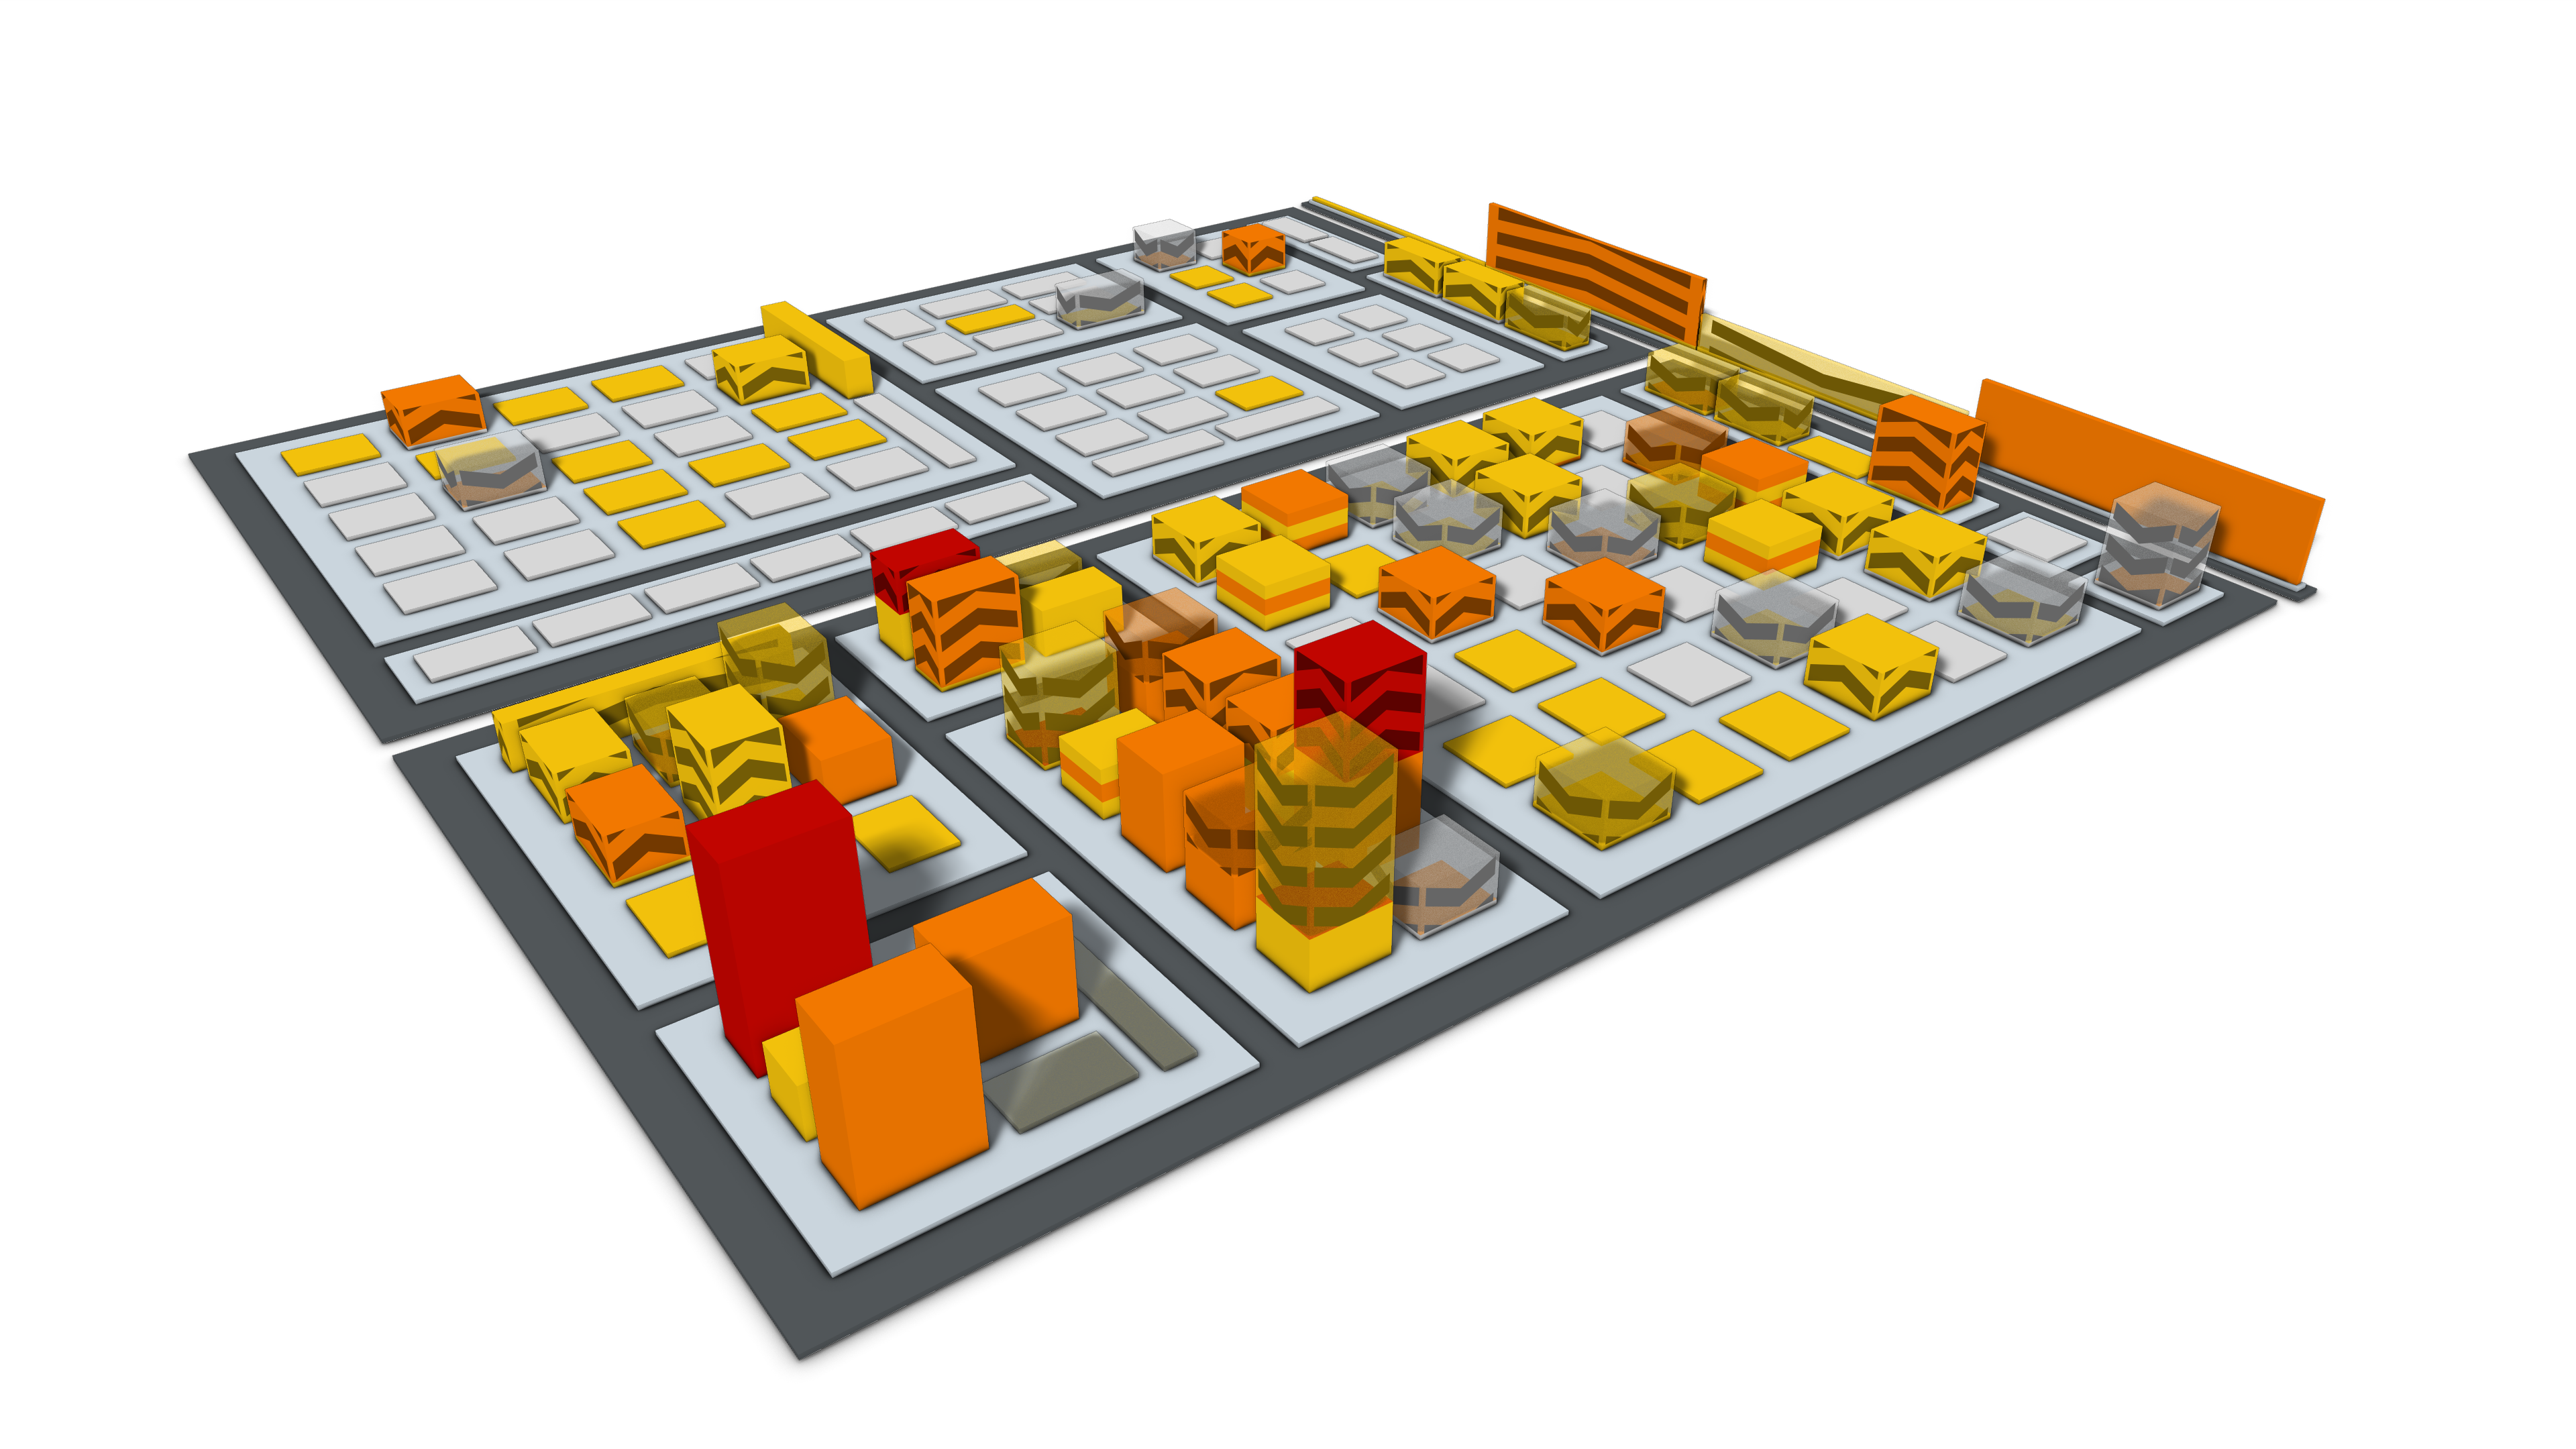
\includegraphics[height=\paperheight]{images/showcase/transparency-and-procedural-texturing}}
\begin{frame}{~}
\end{frame}
}

\begin{frame}[c]{~}
    \bigskip

    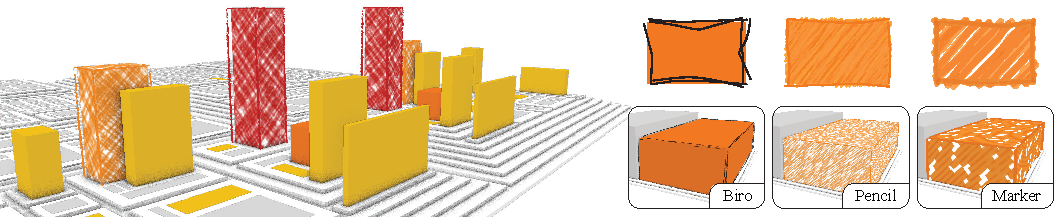
\includegraphics[width=\textwidth]{images/showcase/sketchy-teaser2}
    \medskip

    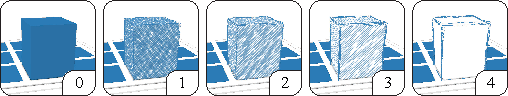
\includegraphics[width=\textwidth]{images/showcase/sketchy-stylization-order-pencil}

\end{frame}

{
\usebackgroundtemplate{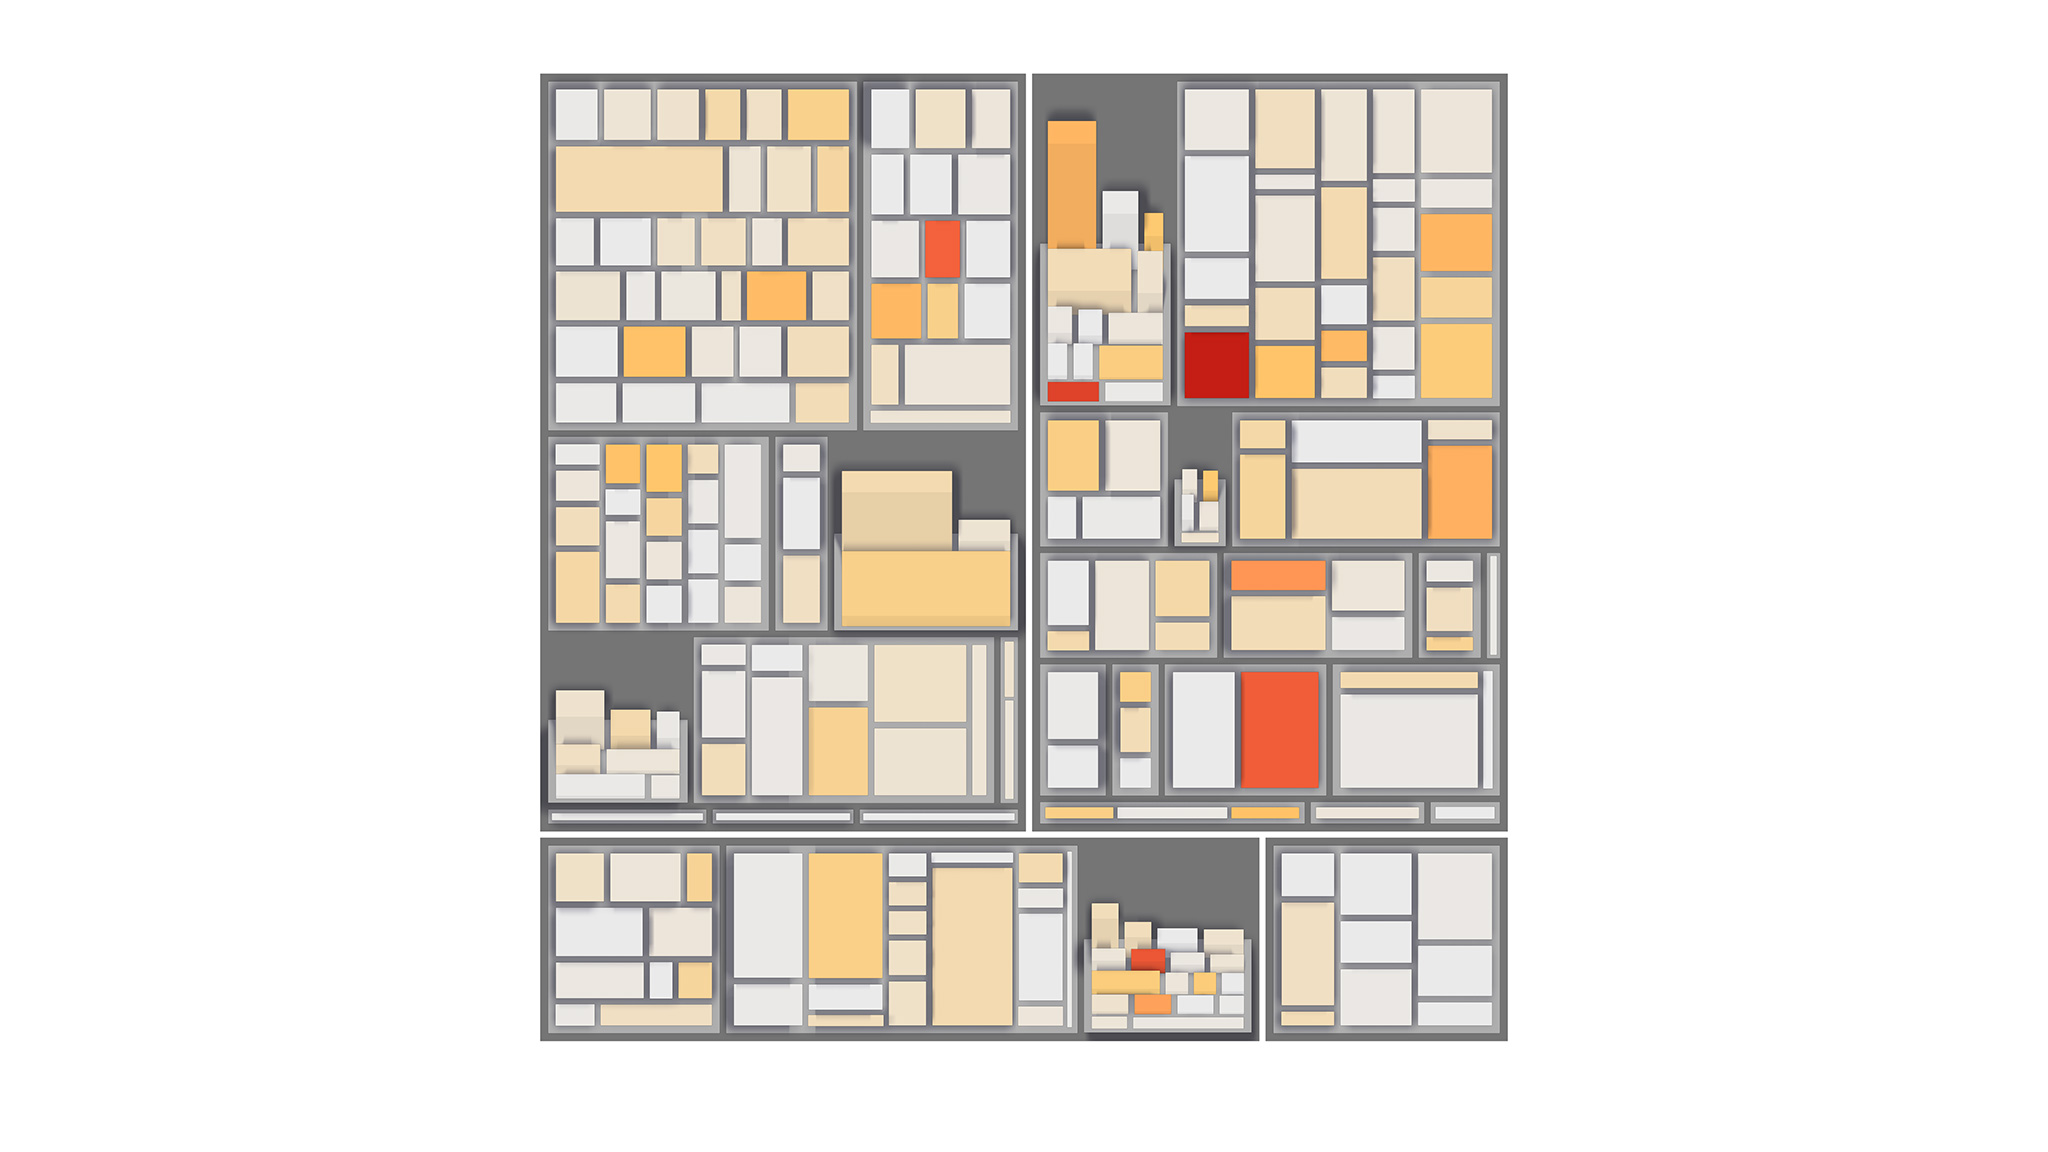
\includegraphics[height=\paperheight]{images/showcase/mixed-projection}}
\begin{frame}{~}
\end{frame}
}

{
\usebackgroundtemplate{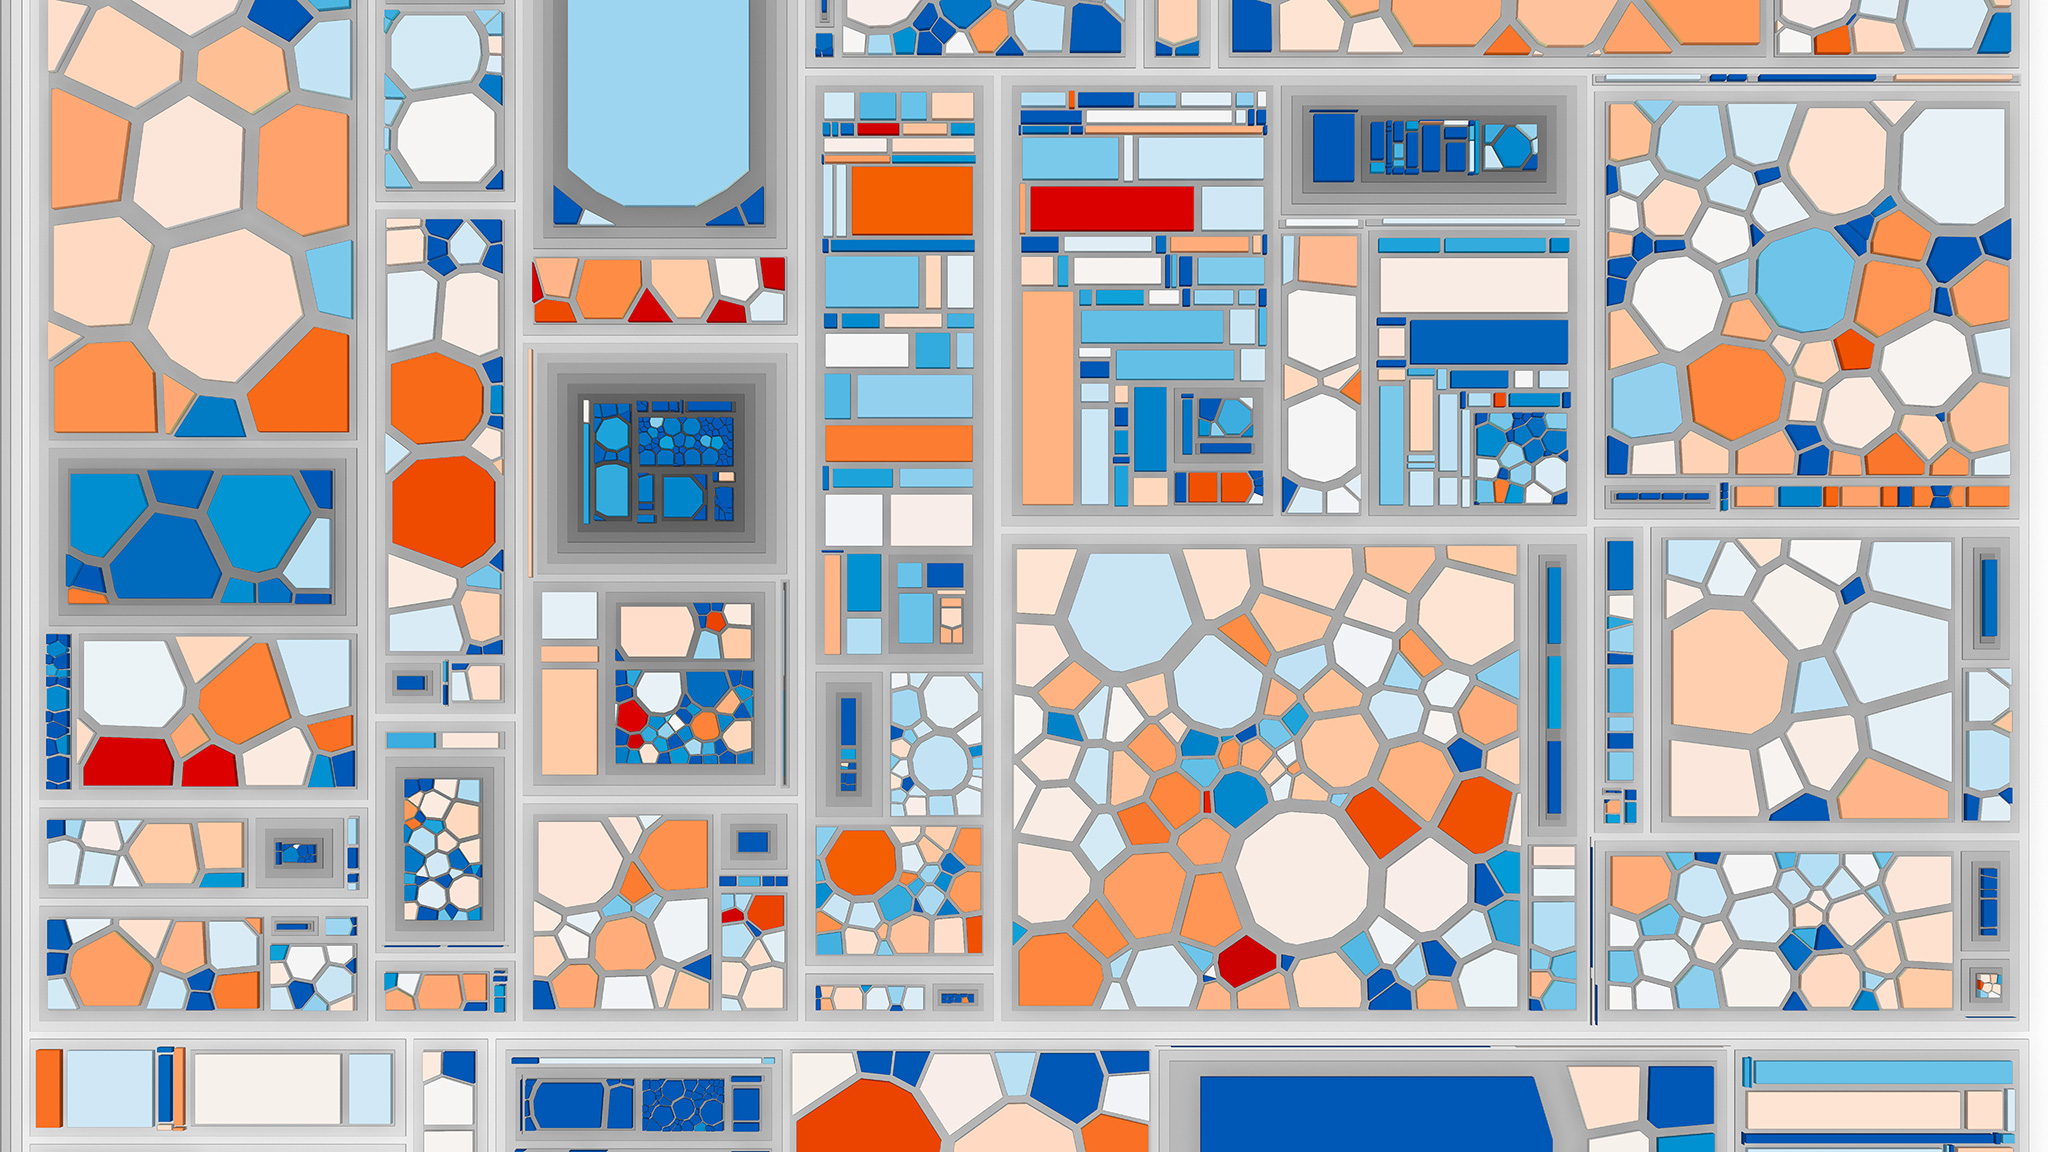
\includegraphics[height=\paperheight]{images/showcase/mixed-layout-2}}
\begin{frame}{~}
\end{frame}
}

{
\usebackgroundtemplate{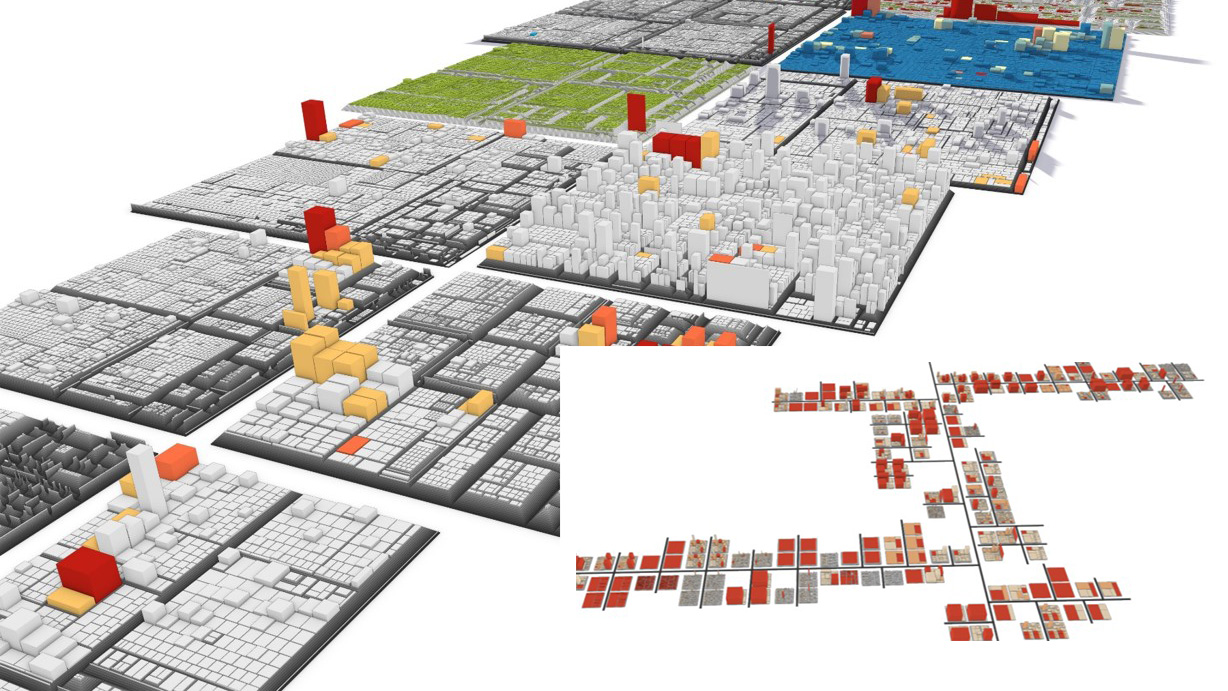
\includegraphics[height=\paperheight]{images/showcase/evo-cities}}
\begin{frame}{~}
\end{frame}
}

{
\usebackgroundtemplate{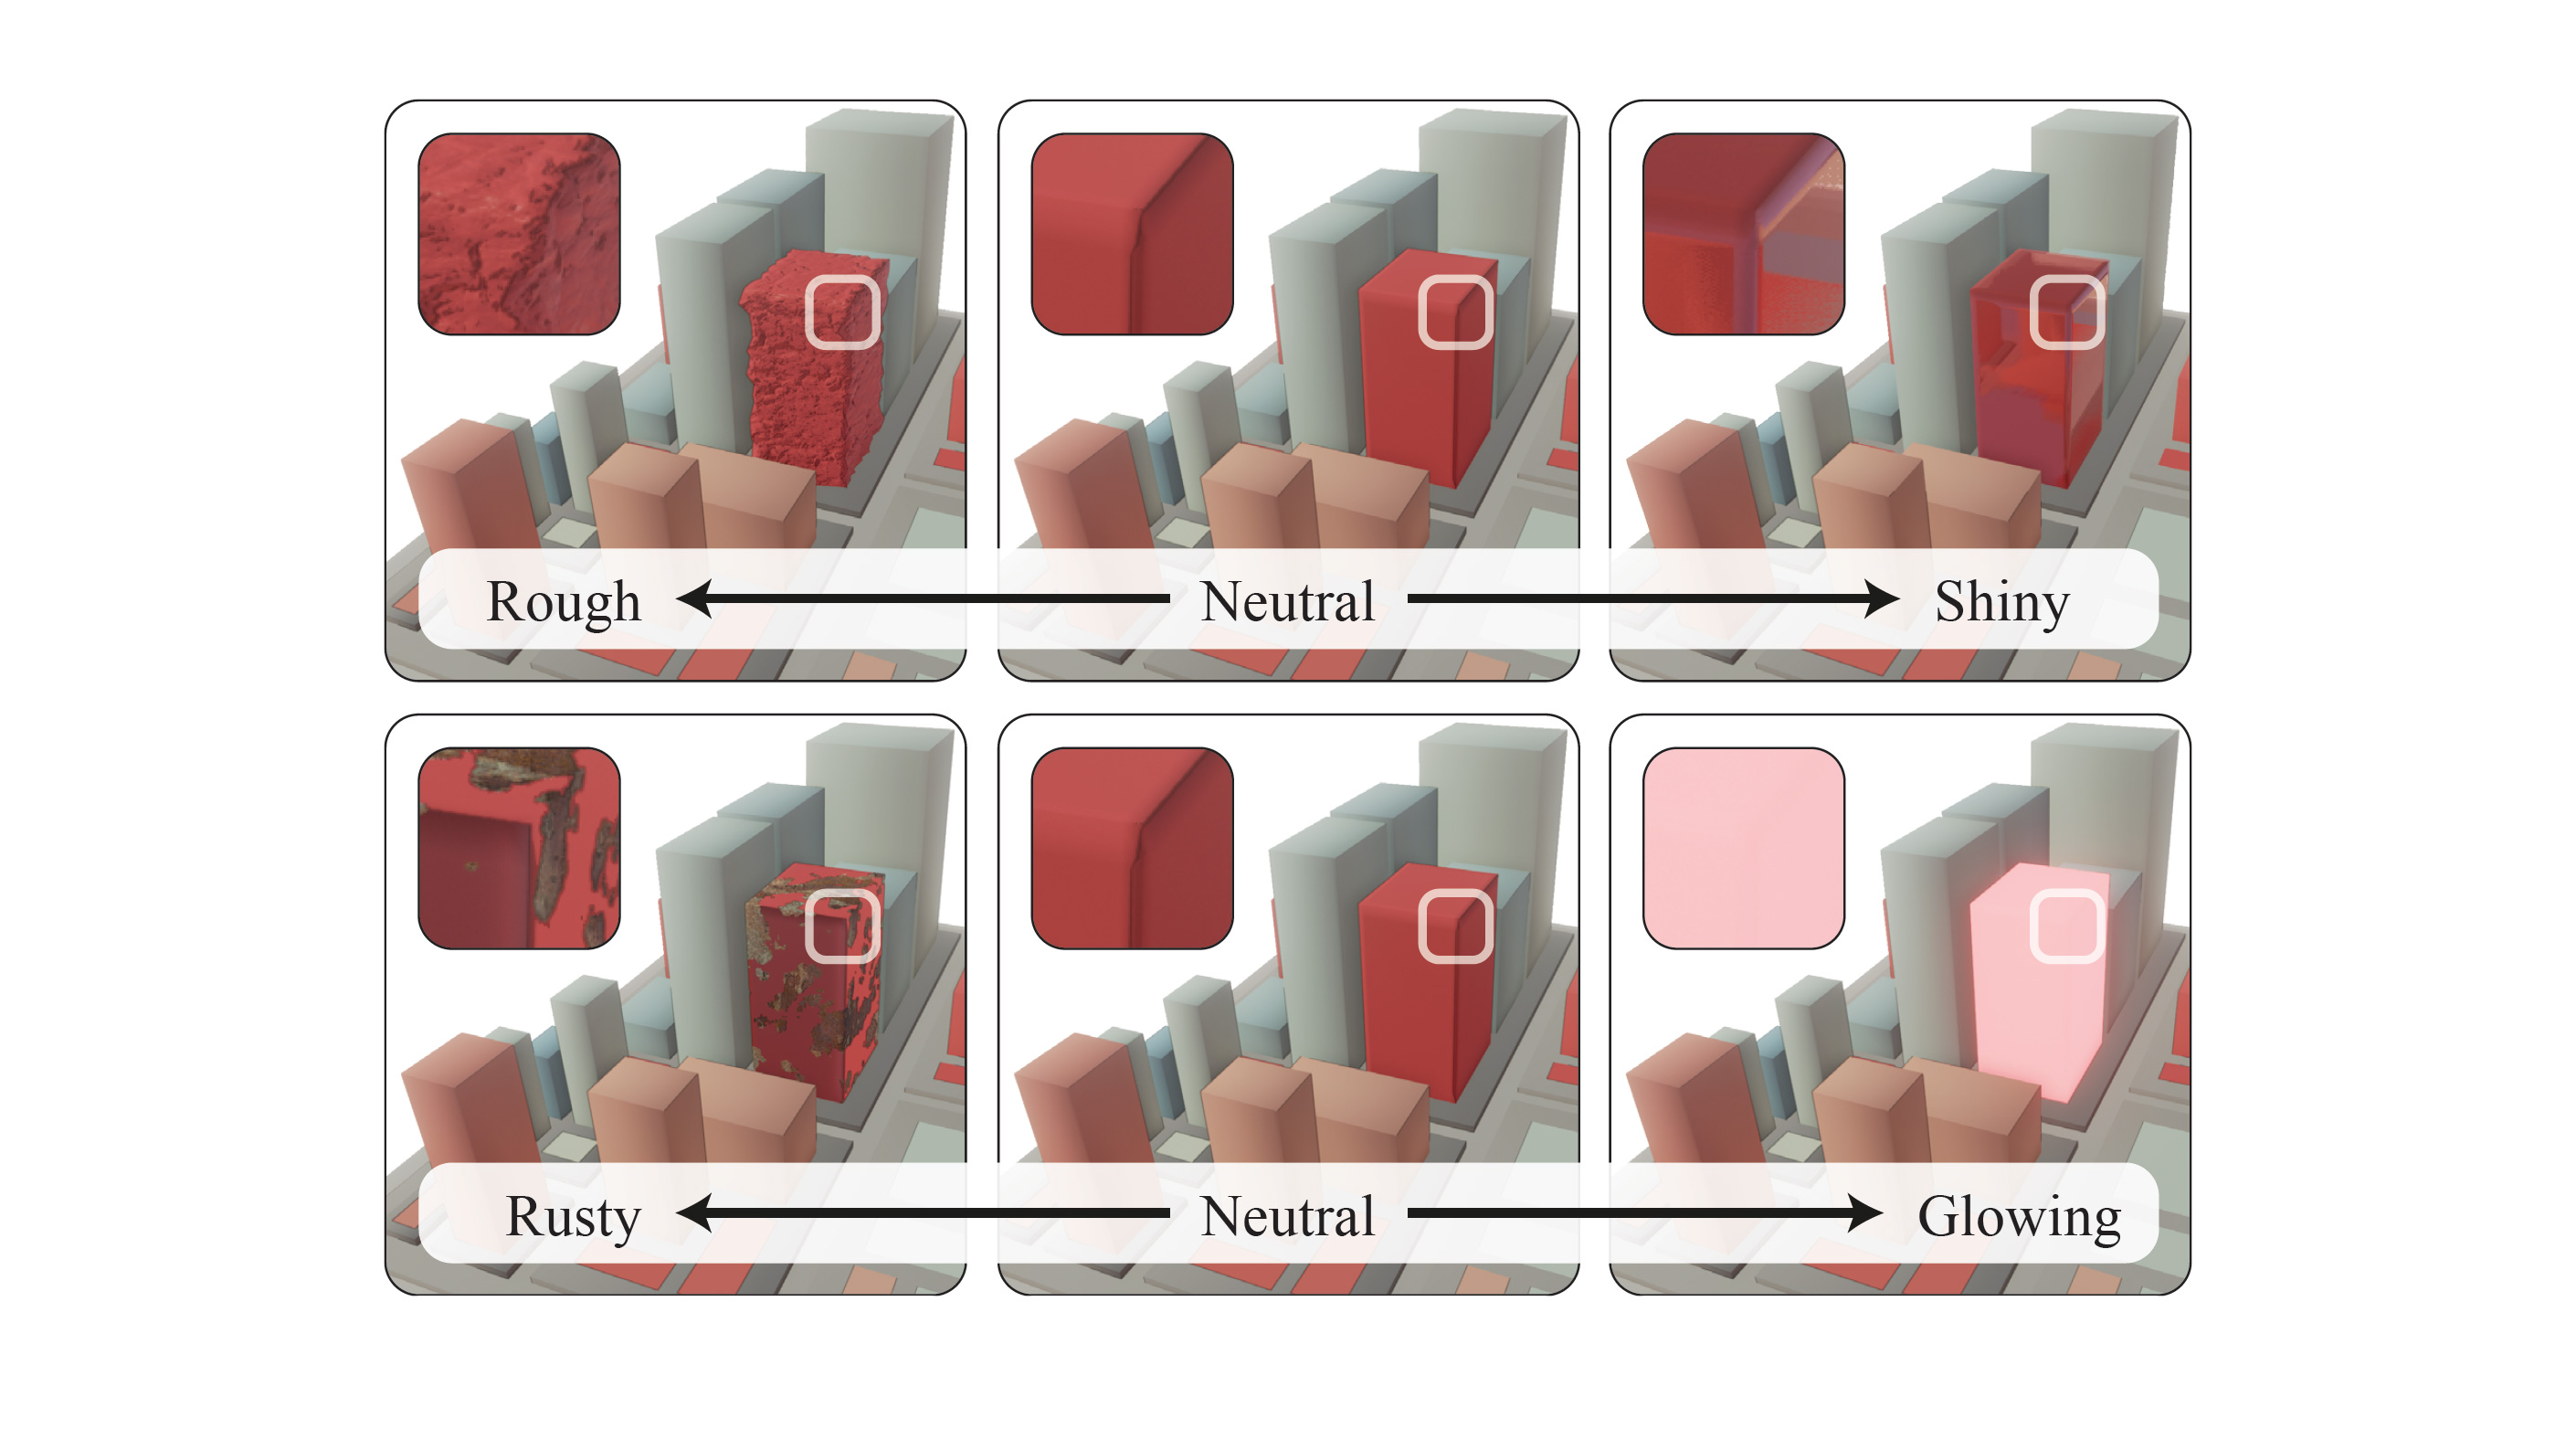
\includegraphics[height=\paperheight]{images/showcase/natural-metaphors}}
\begin{frame}{~}
\end{frame}
}

{
\usebackgroundtemplate{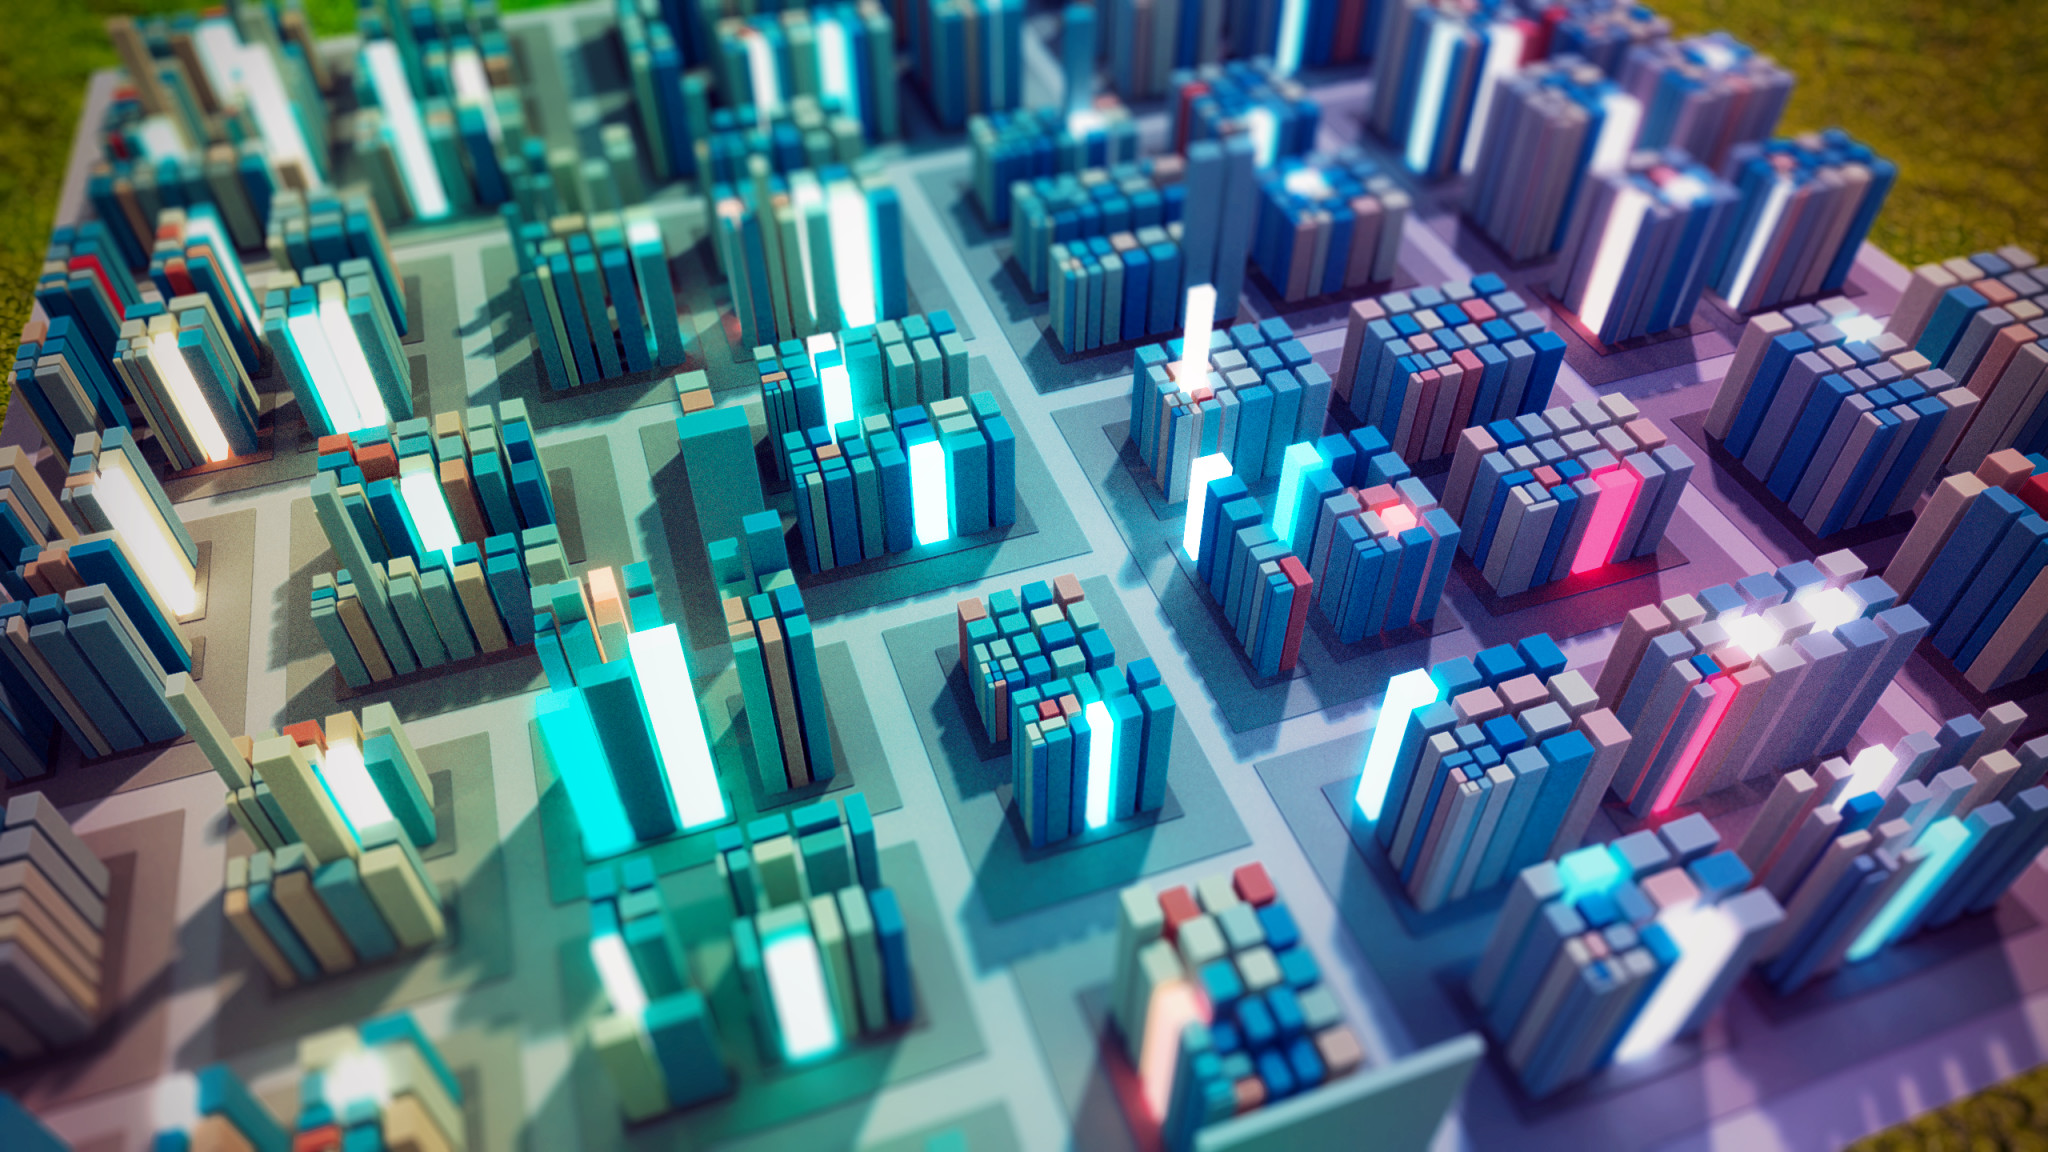
\includegraphics[height=\paperheight]{images/showcase/glow-light}}
\begin{frame}{~}
\end{frame}
}

{
\usebackgroundtemplate{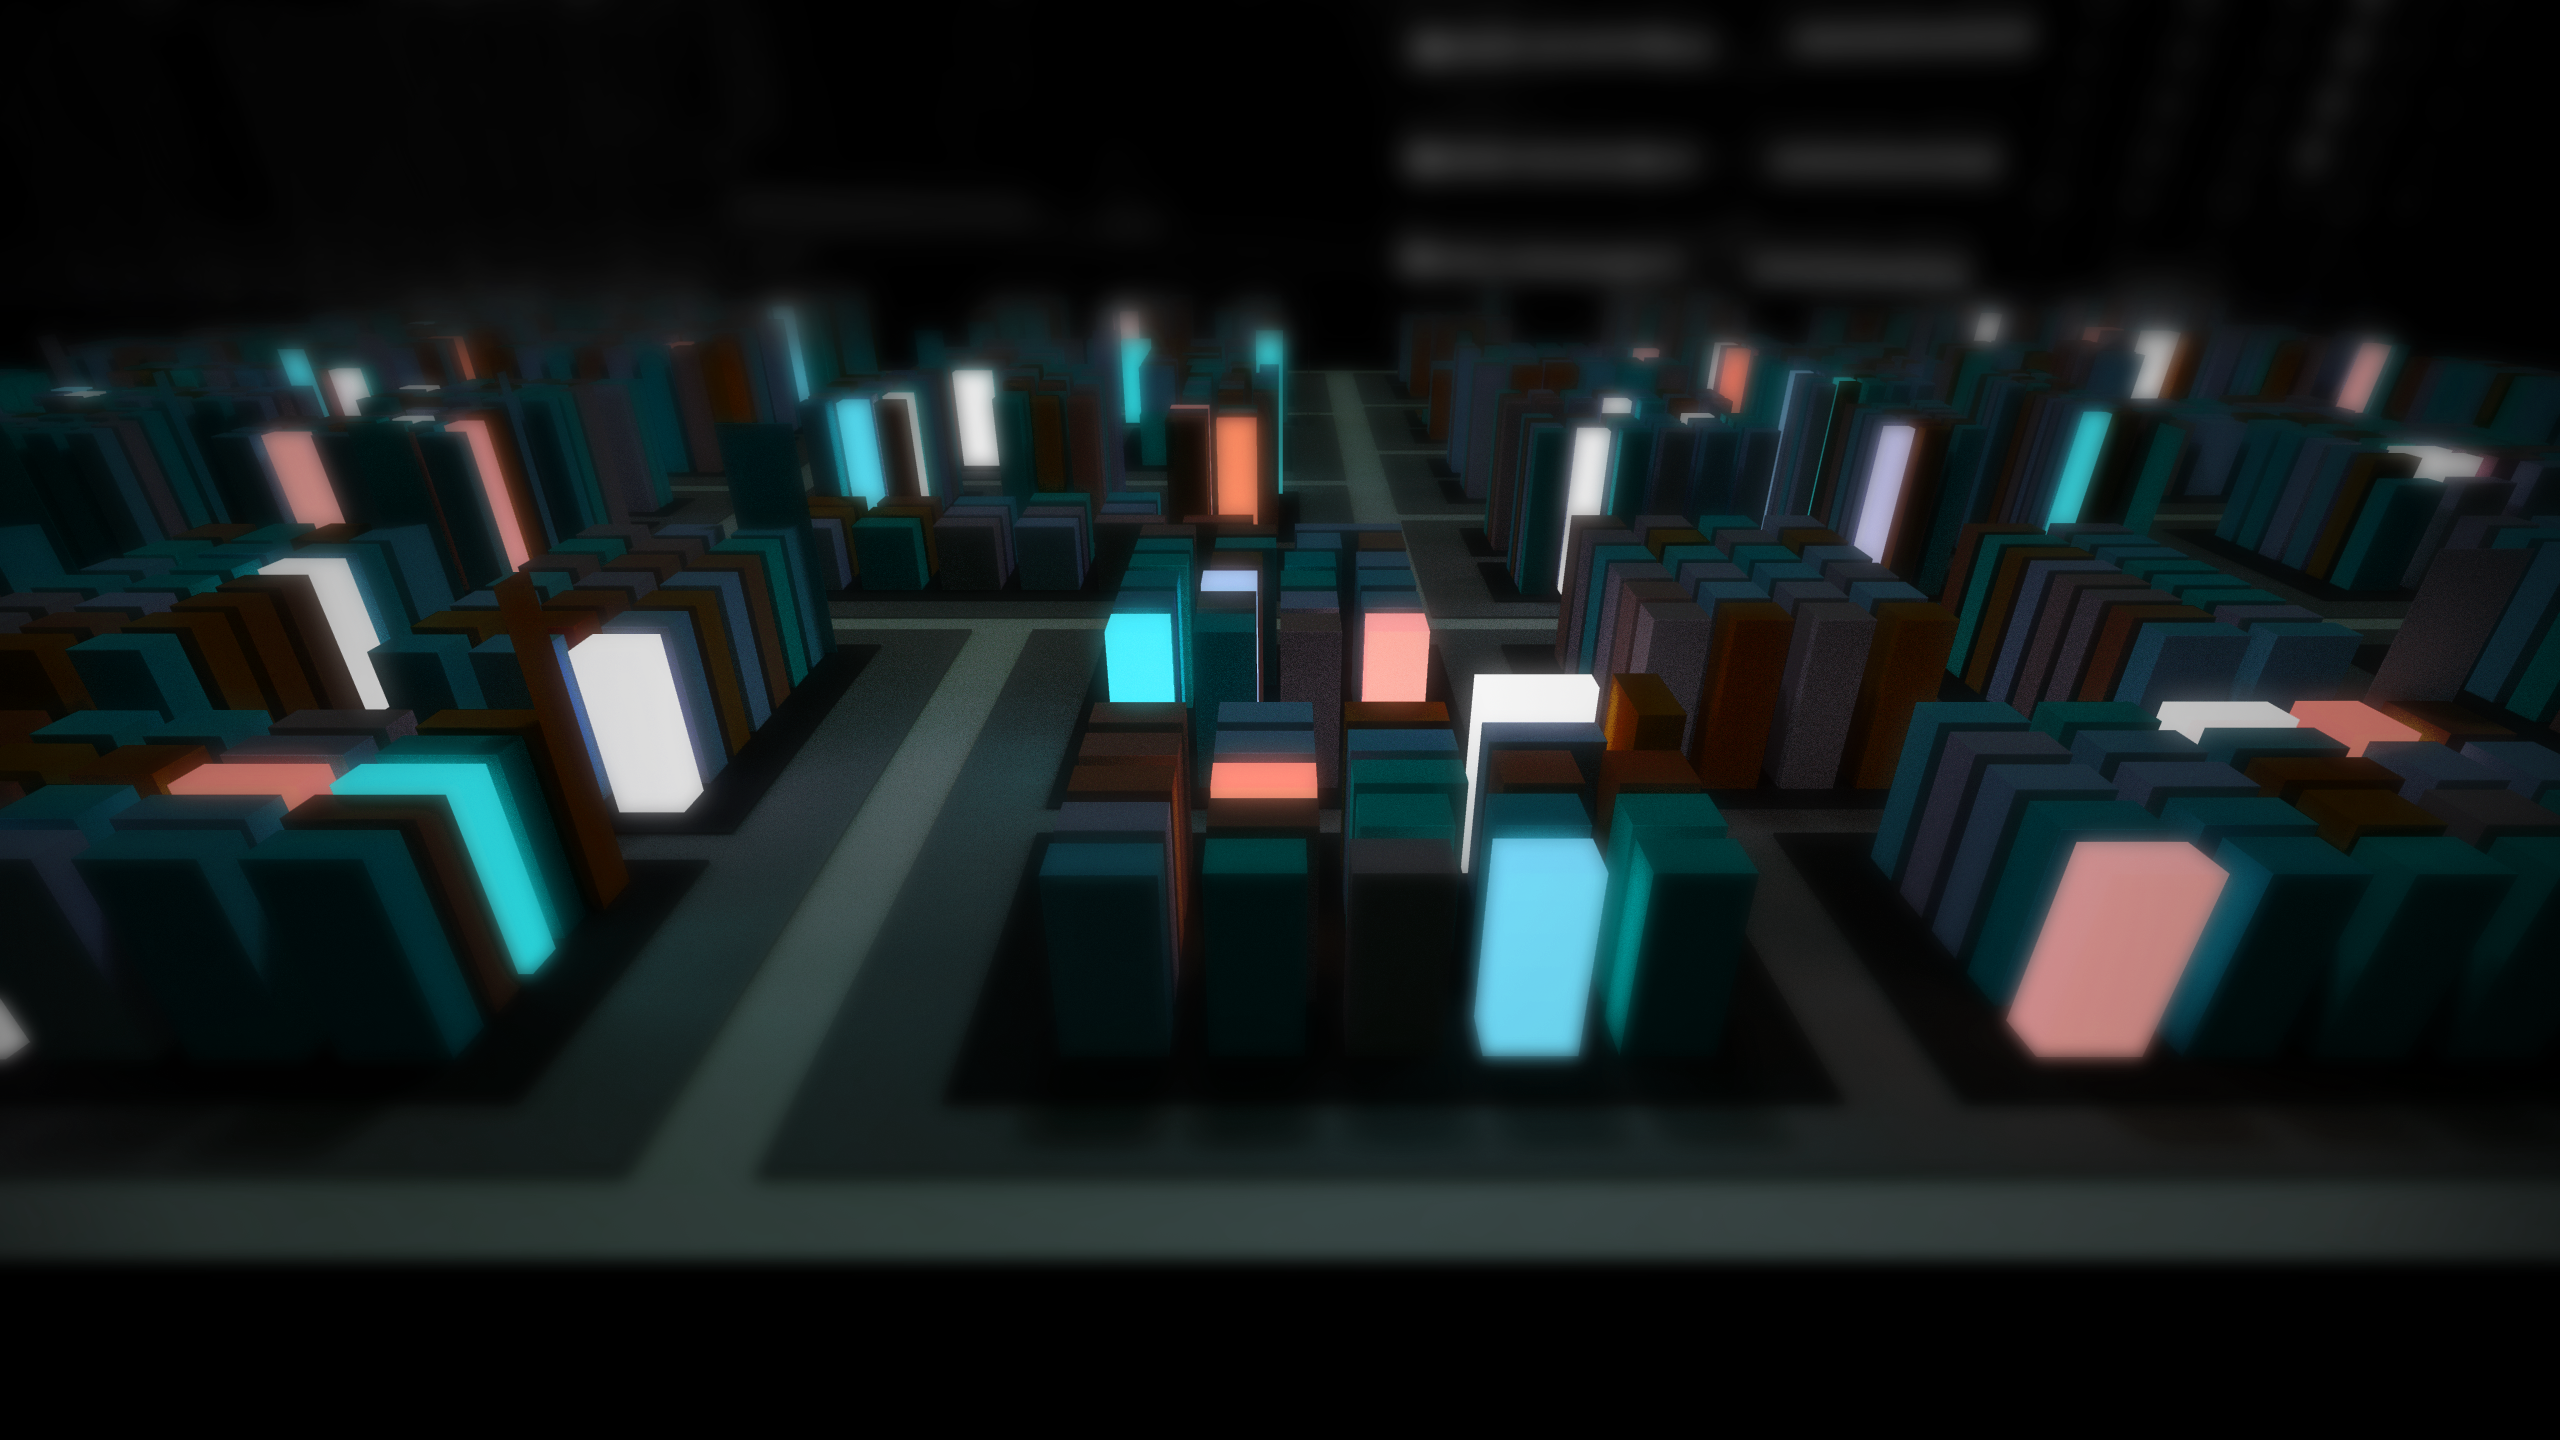
\includegraphics[height=\paperheight]{images/showcase/glow-dark}}
\begin{frame}{~}
\end{frame}
}

{
\usebackgroundtemplate{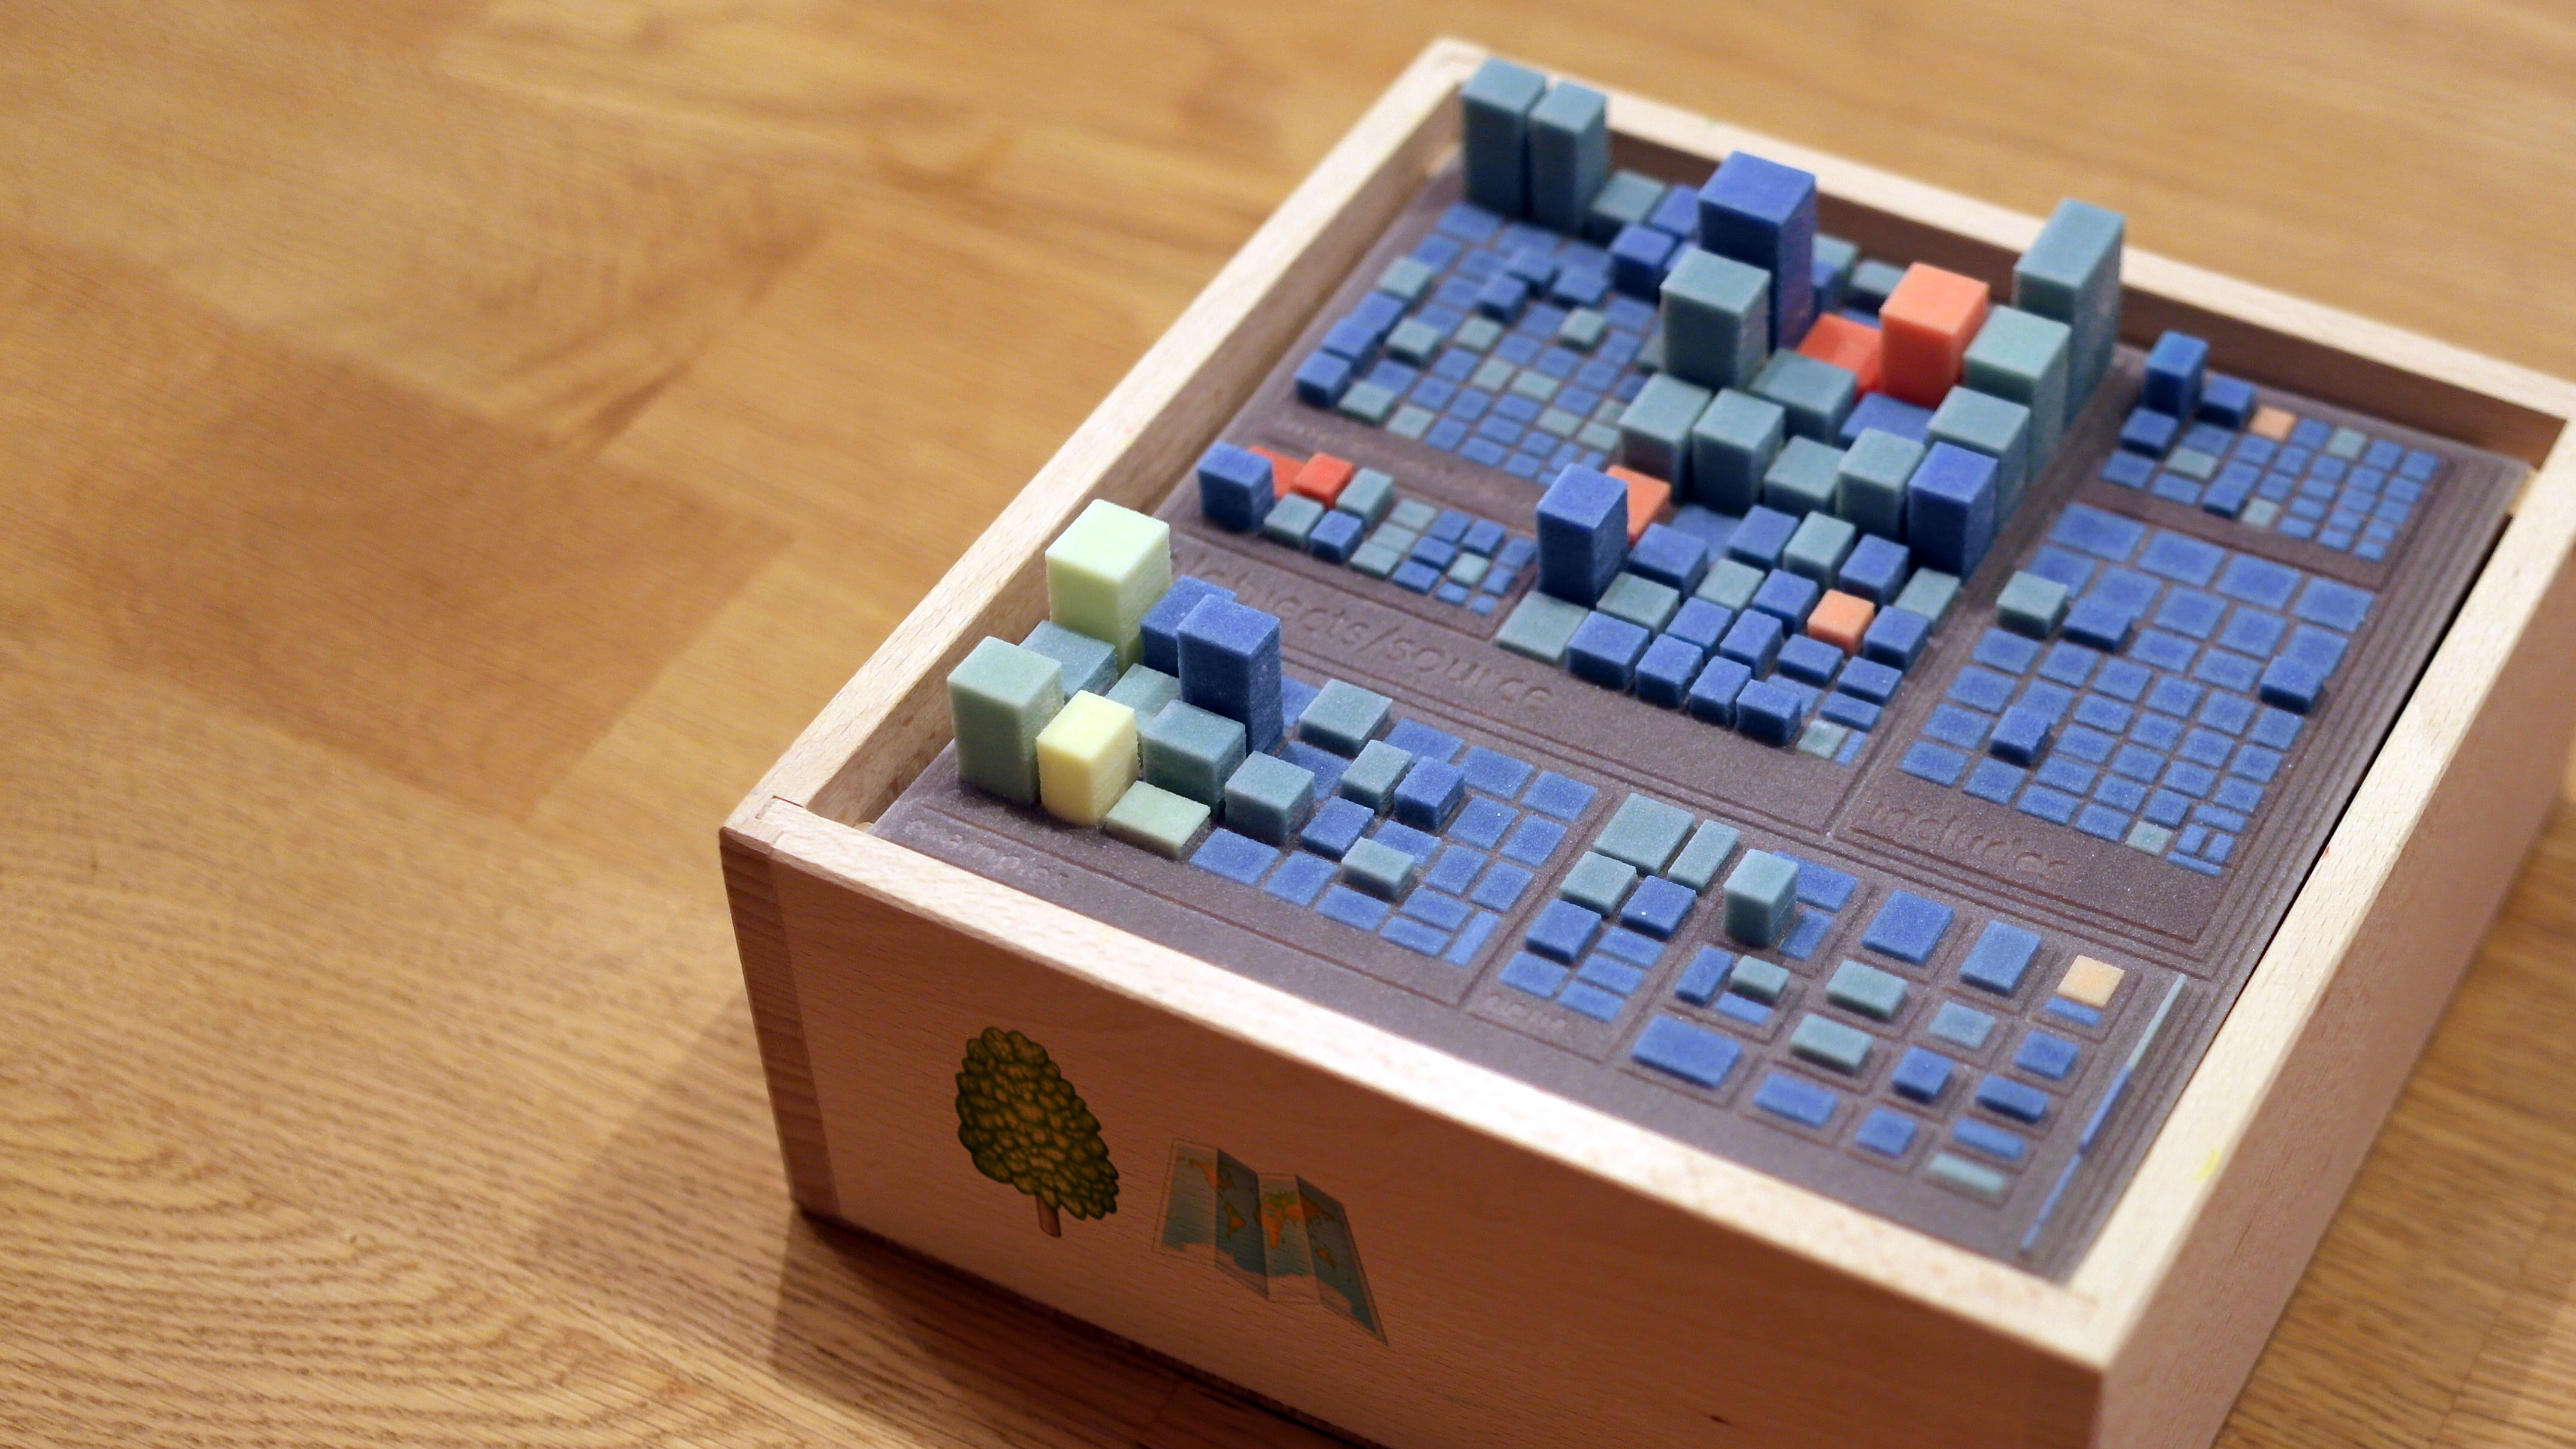
\includegraphics[height=\paperheight]{images/showcase/printed}}
\begin{frame}{~}
\end{frame}
}

{
\usebackgroundtemplate{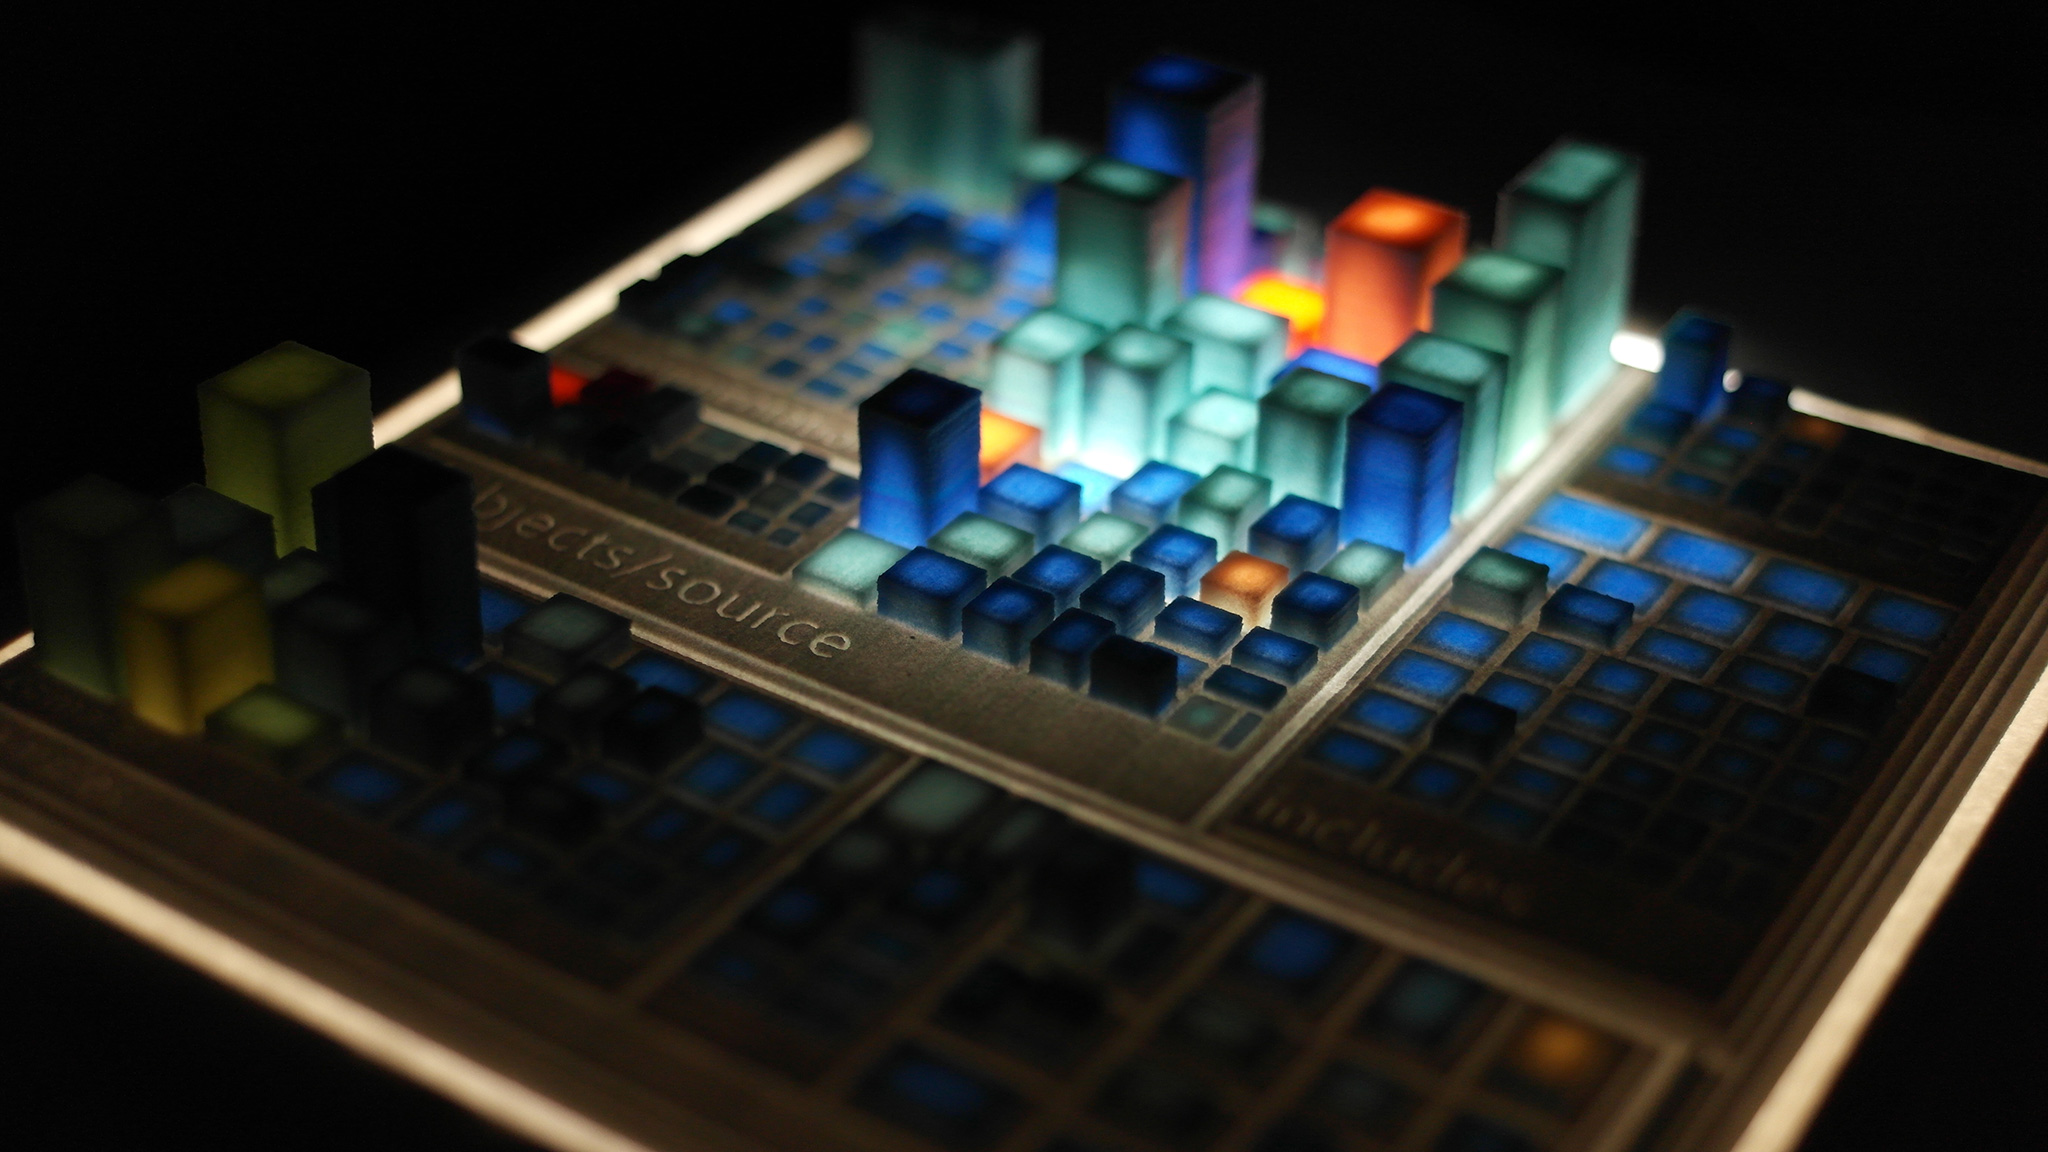
\includegraphics[height=\paperheight]{images/showcase/printed-glow-dark}}
\begin{frame}{~}
\end{frame}
}

{
\usebackgroundtemplate{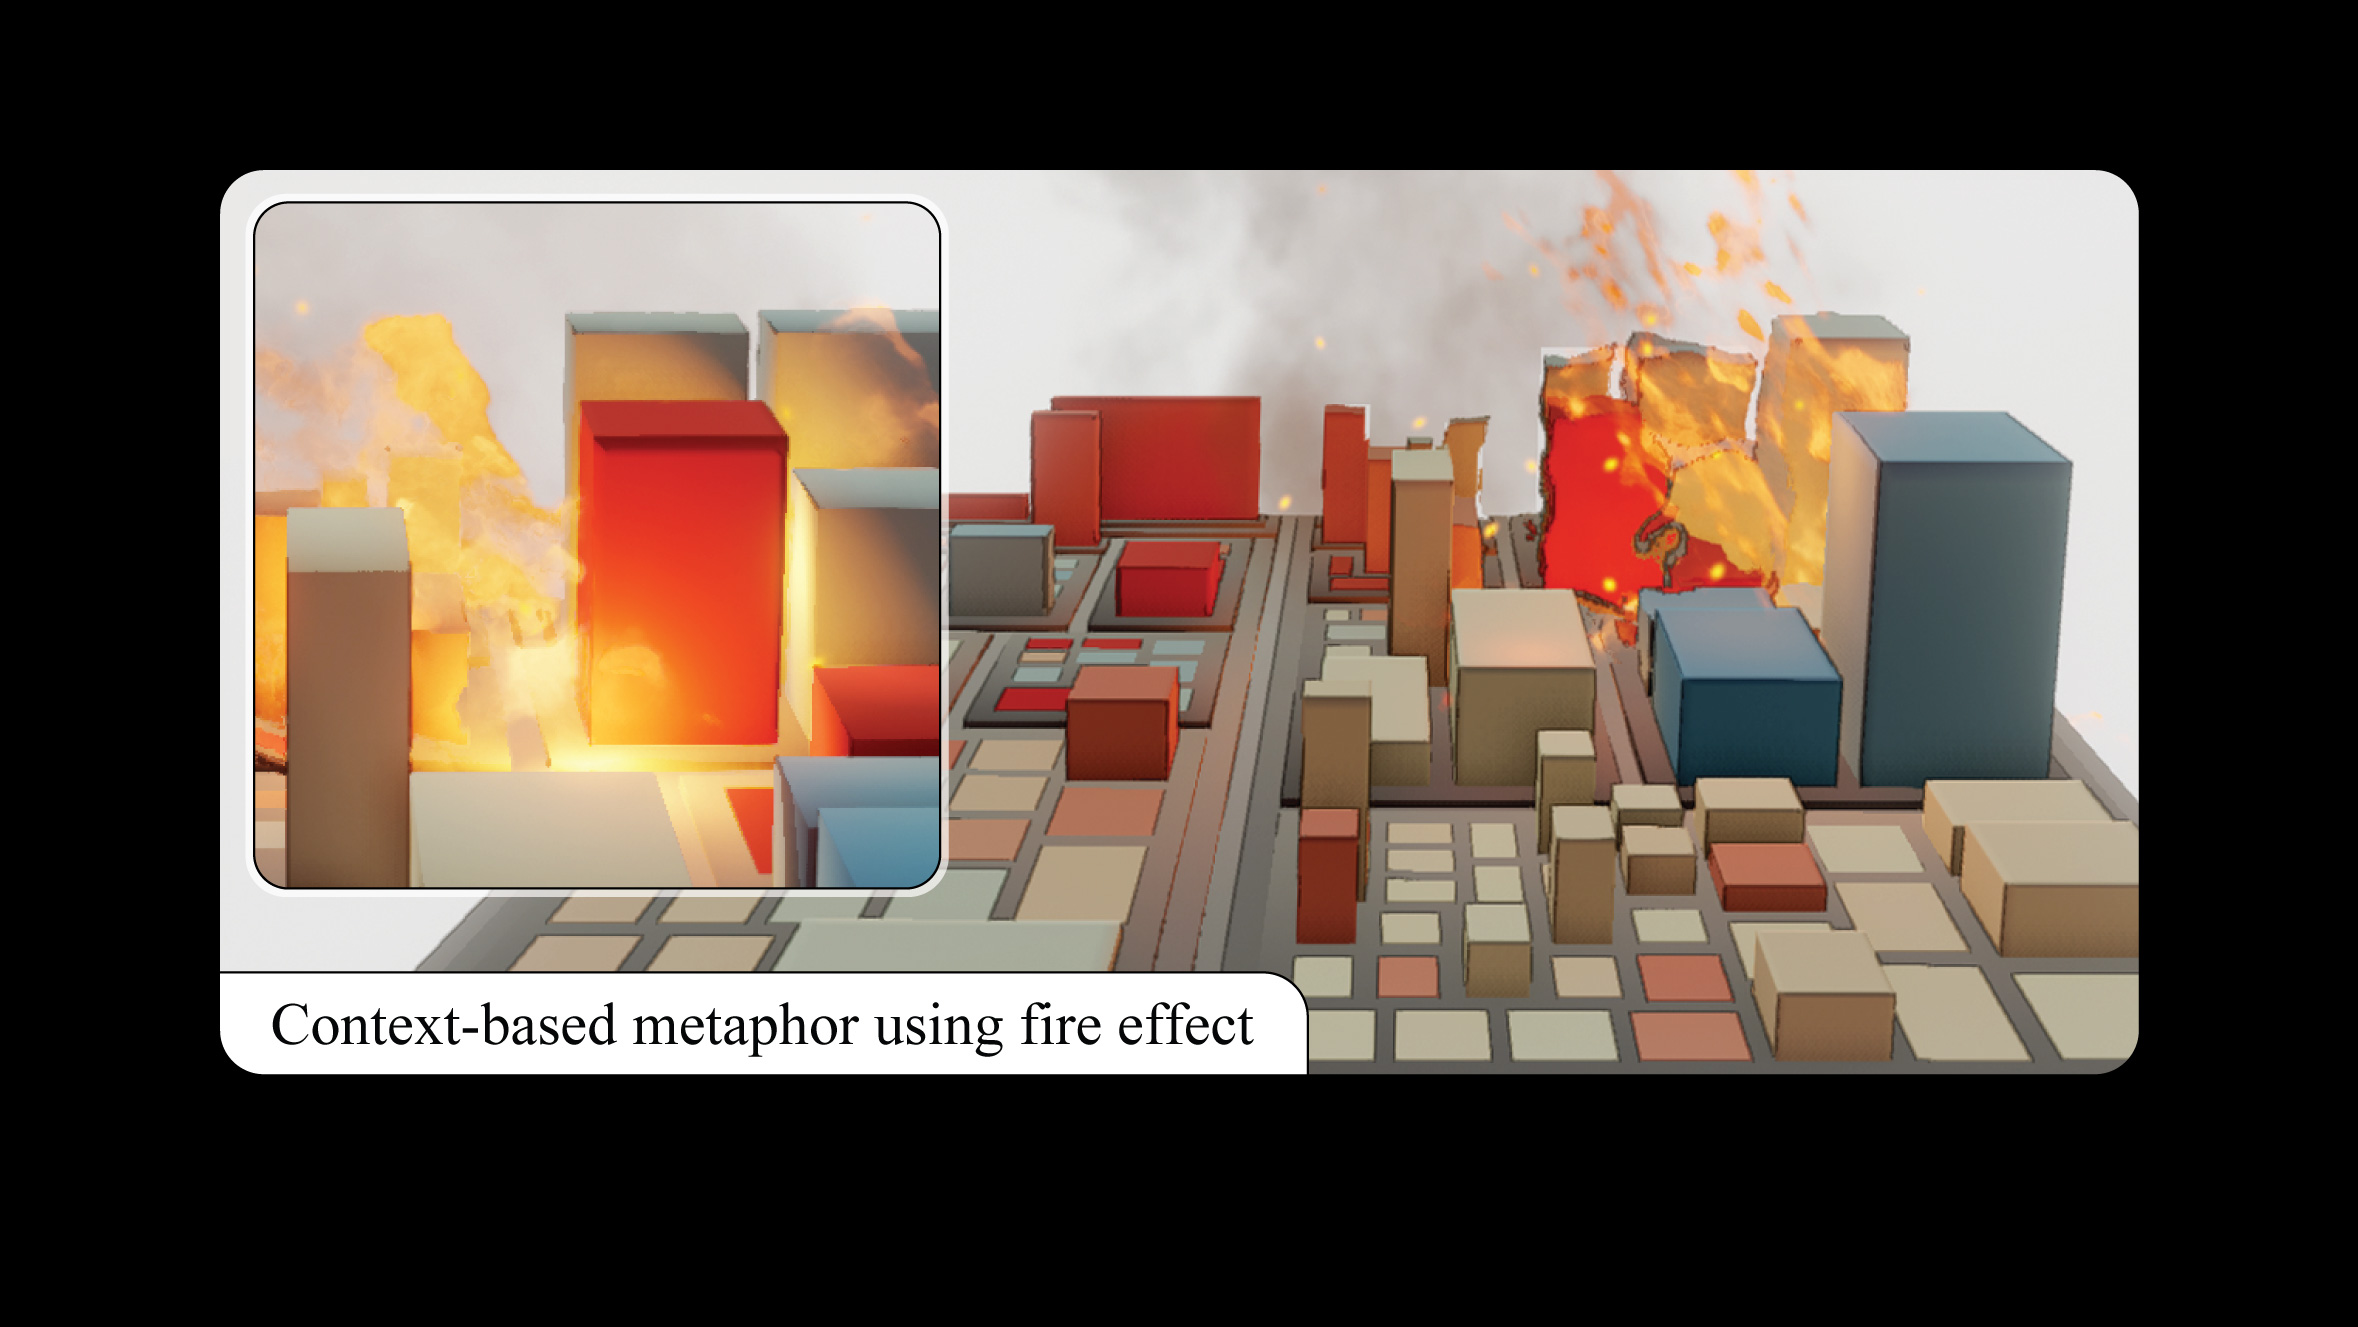
\includegraphics[height=\paperheight]{images/showcase/metaphor-fire}}
\begin{frame}{~}
\end{frame}
}

{
\usebackgroundtemplate{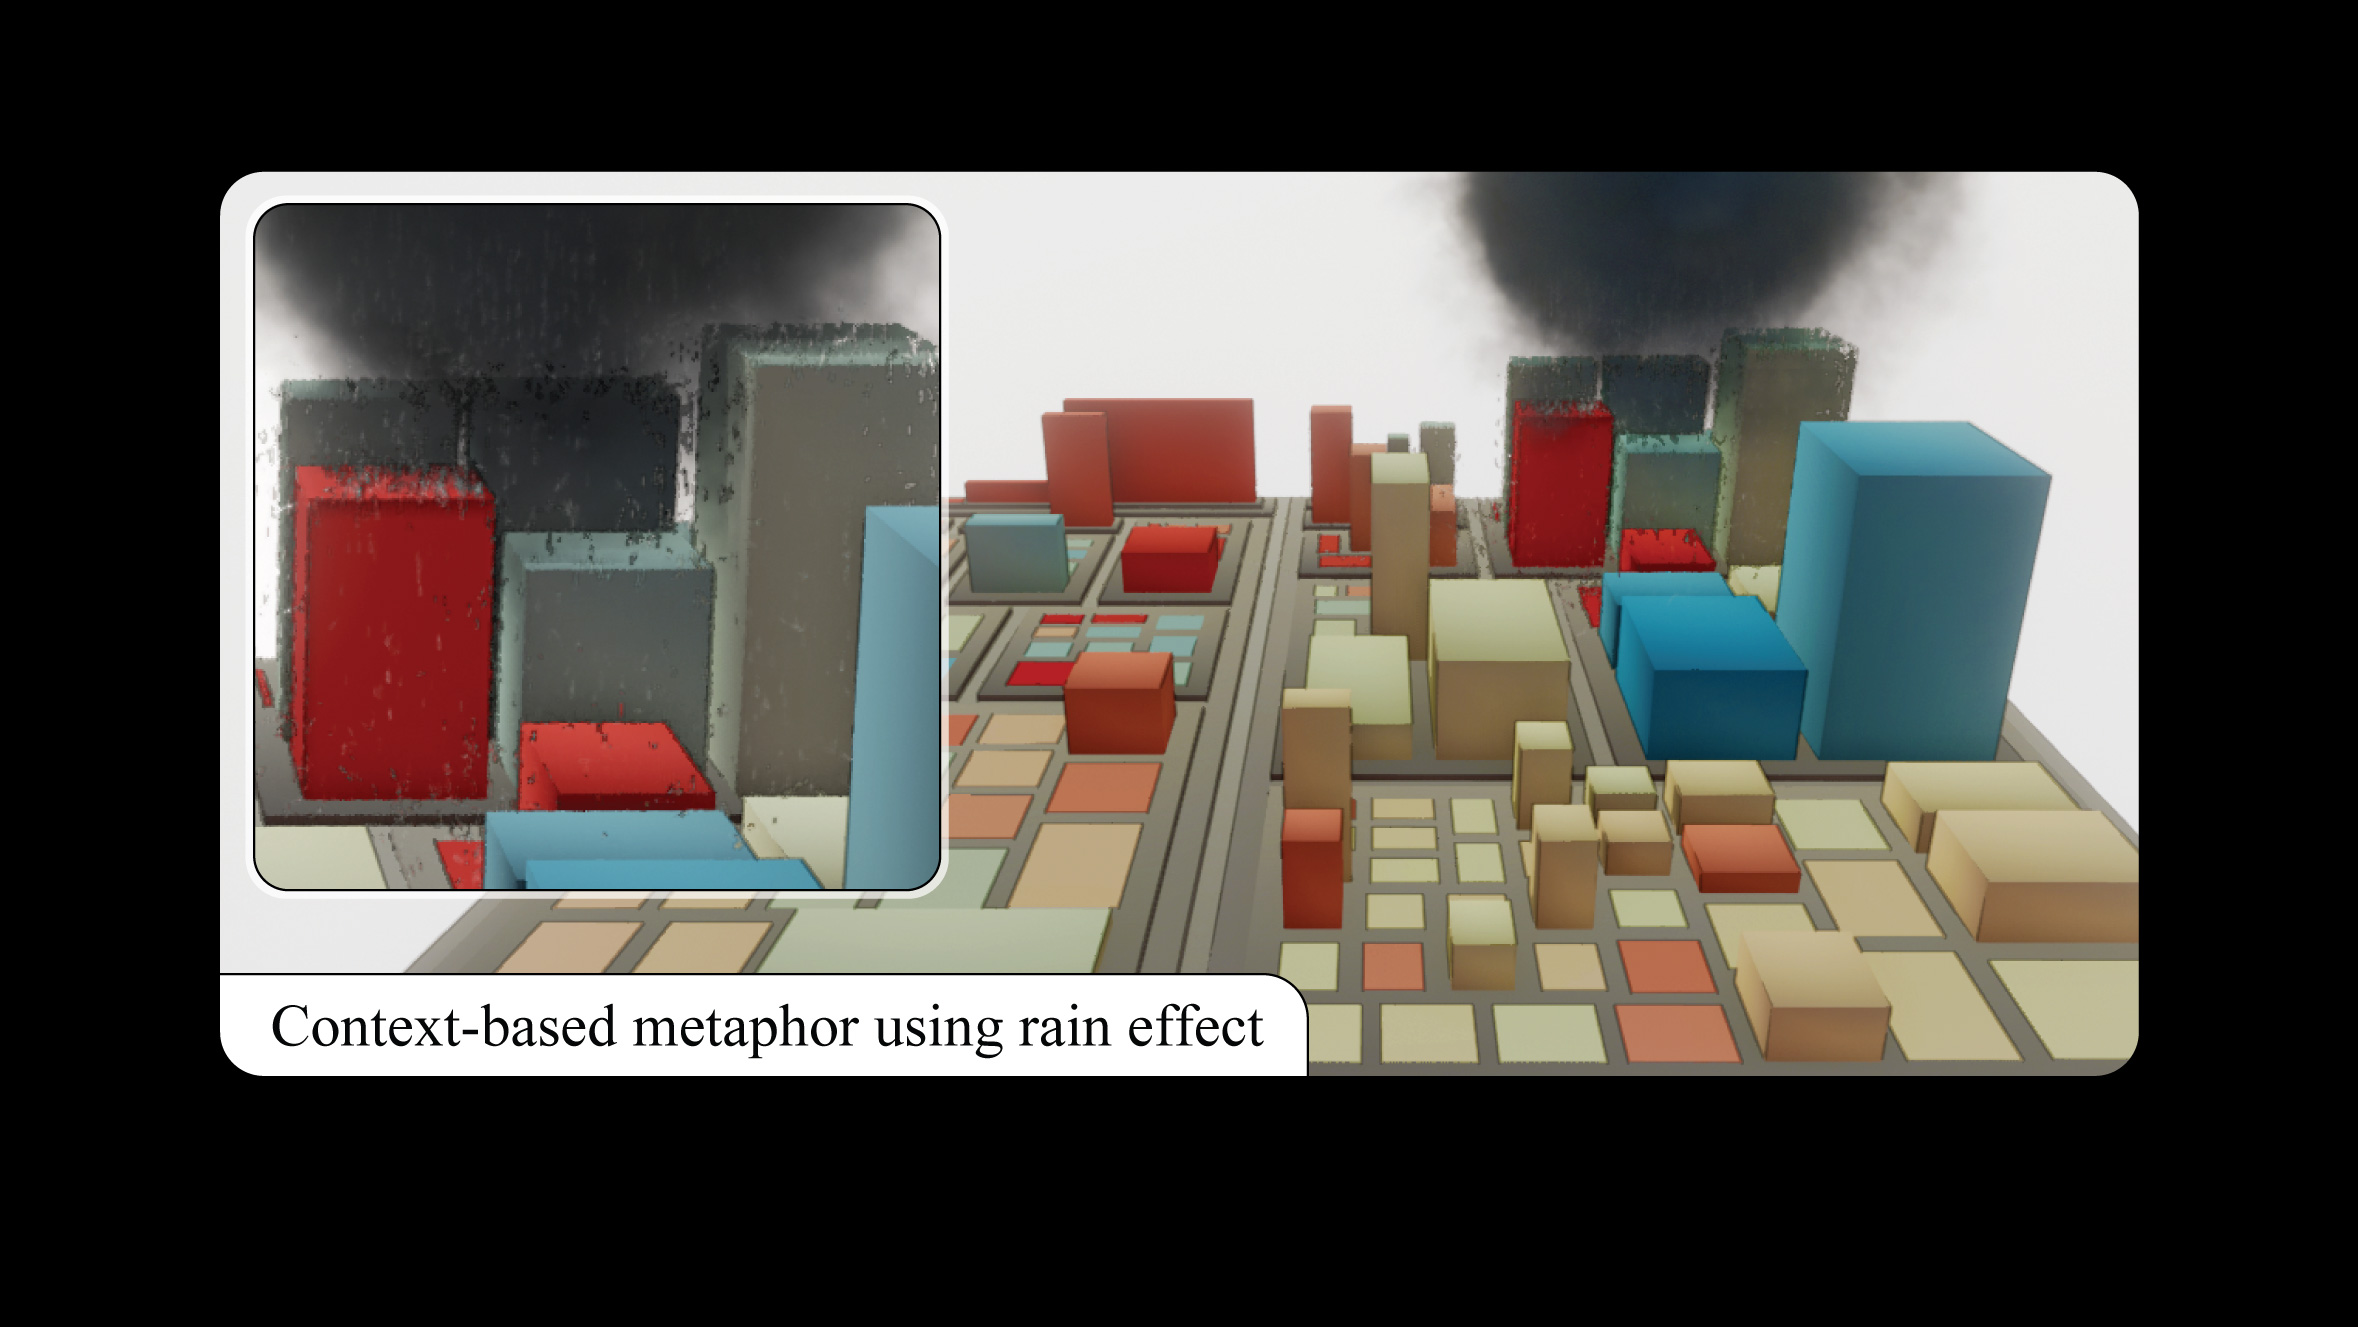
\includegraphics[height=\paperheight]{images/showcase/metaphor-rain}}
\begin{frame}{~}
\end{frame}
}

{
\usebackgroundtemplate{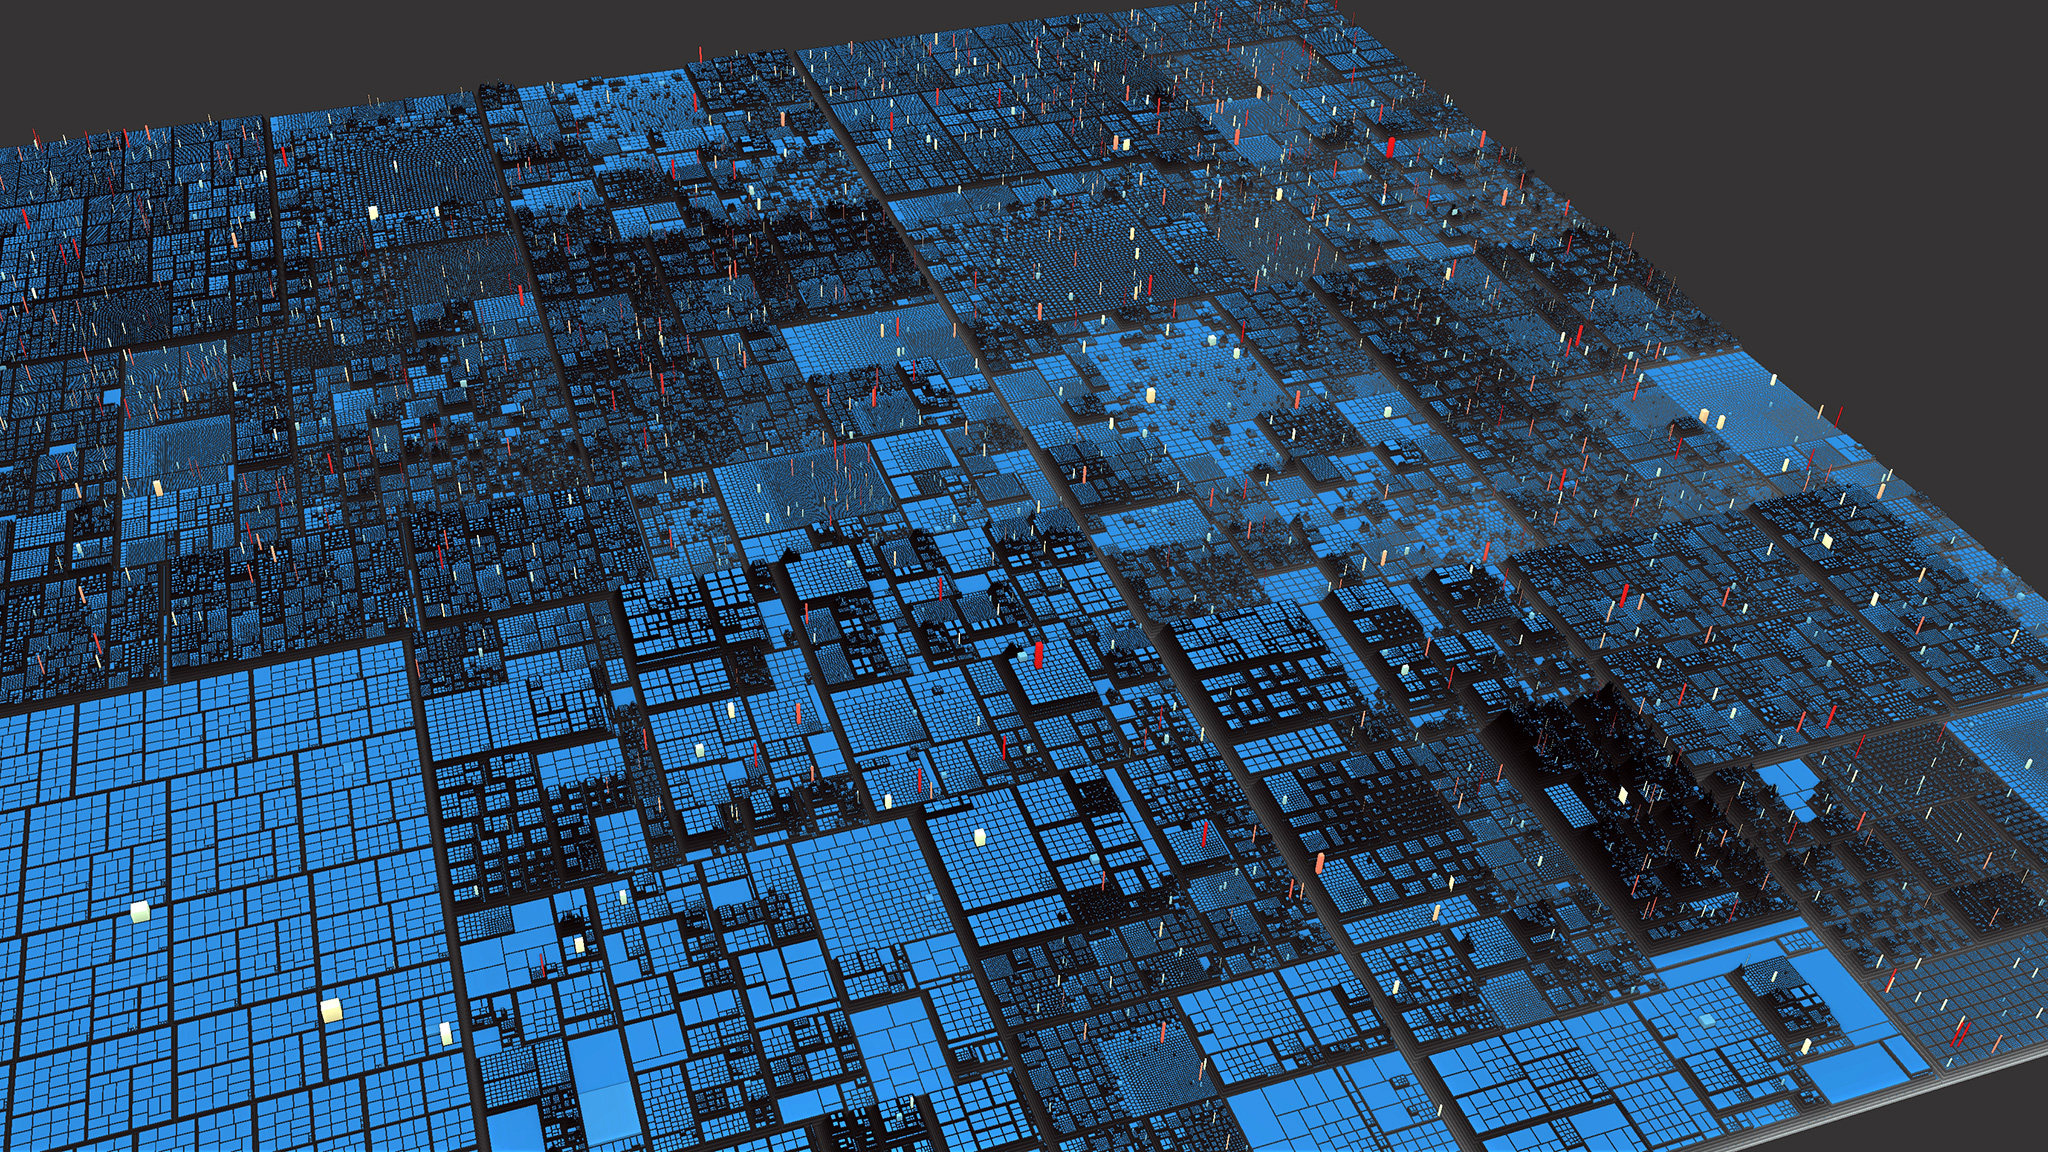
\includegraphics[height=\paperheight]{images/showcase/big-data}}
\begin{frame}{~}
\end{frame}
}

{
\usebackgroundtemplate{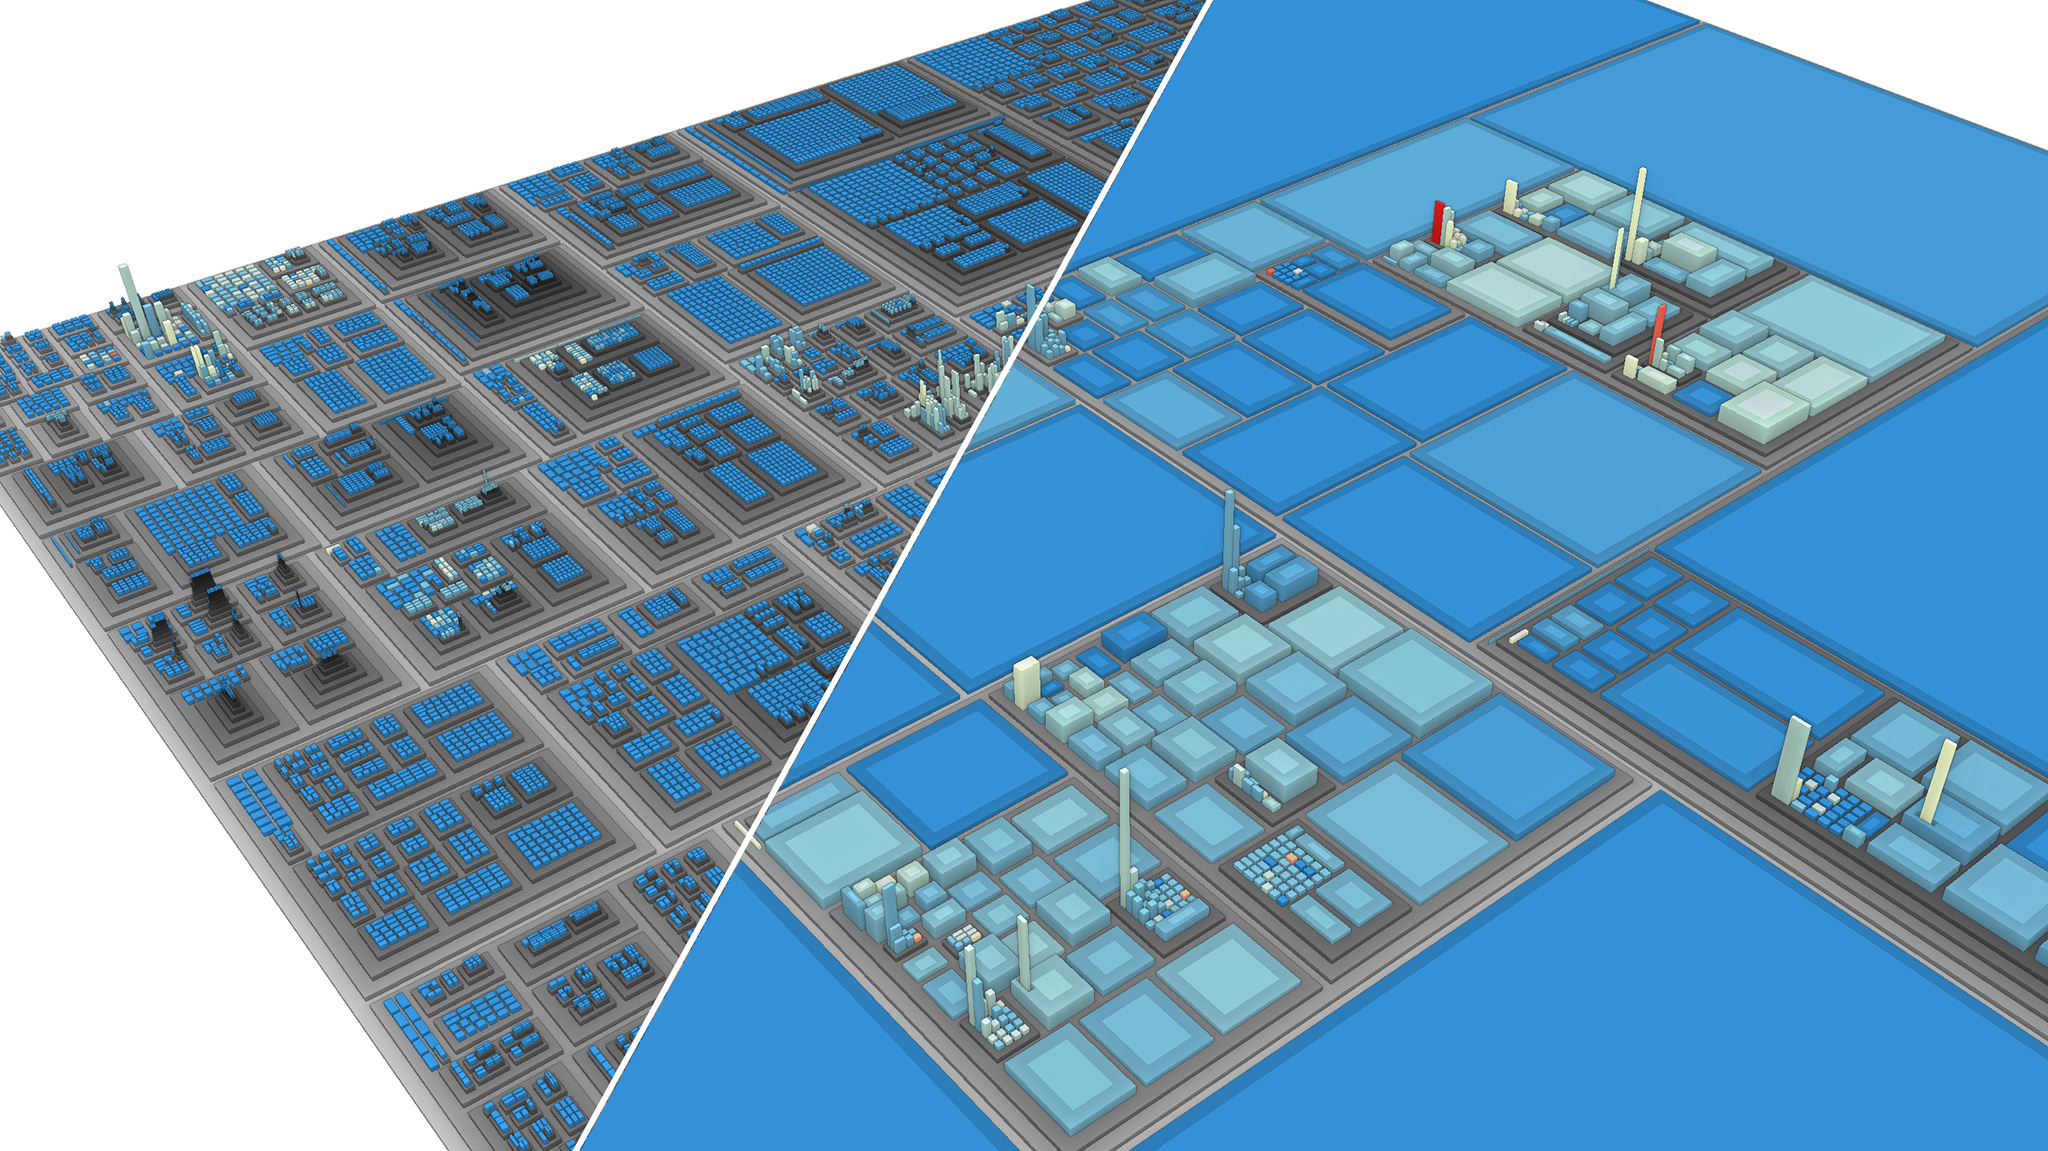
\includegraphics[height=\paperheight]{images/showcase/big-data-aggregated}}
\begin{frame}{~}
\end{frame}
}

{
\usebackgroundtemplate{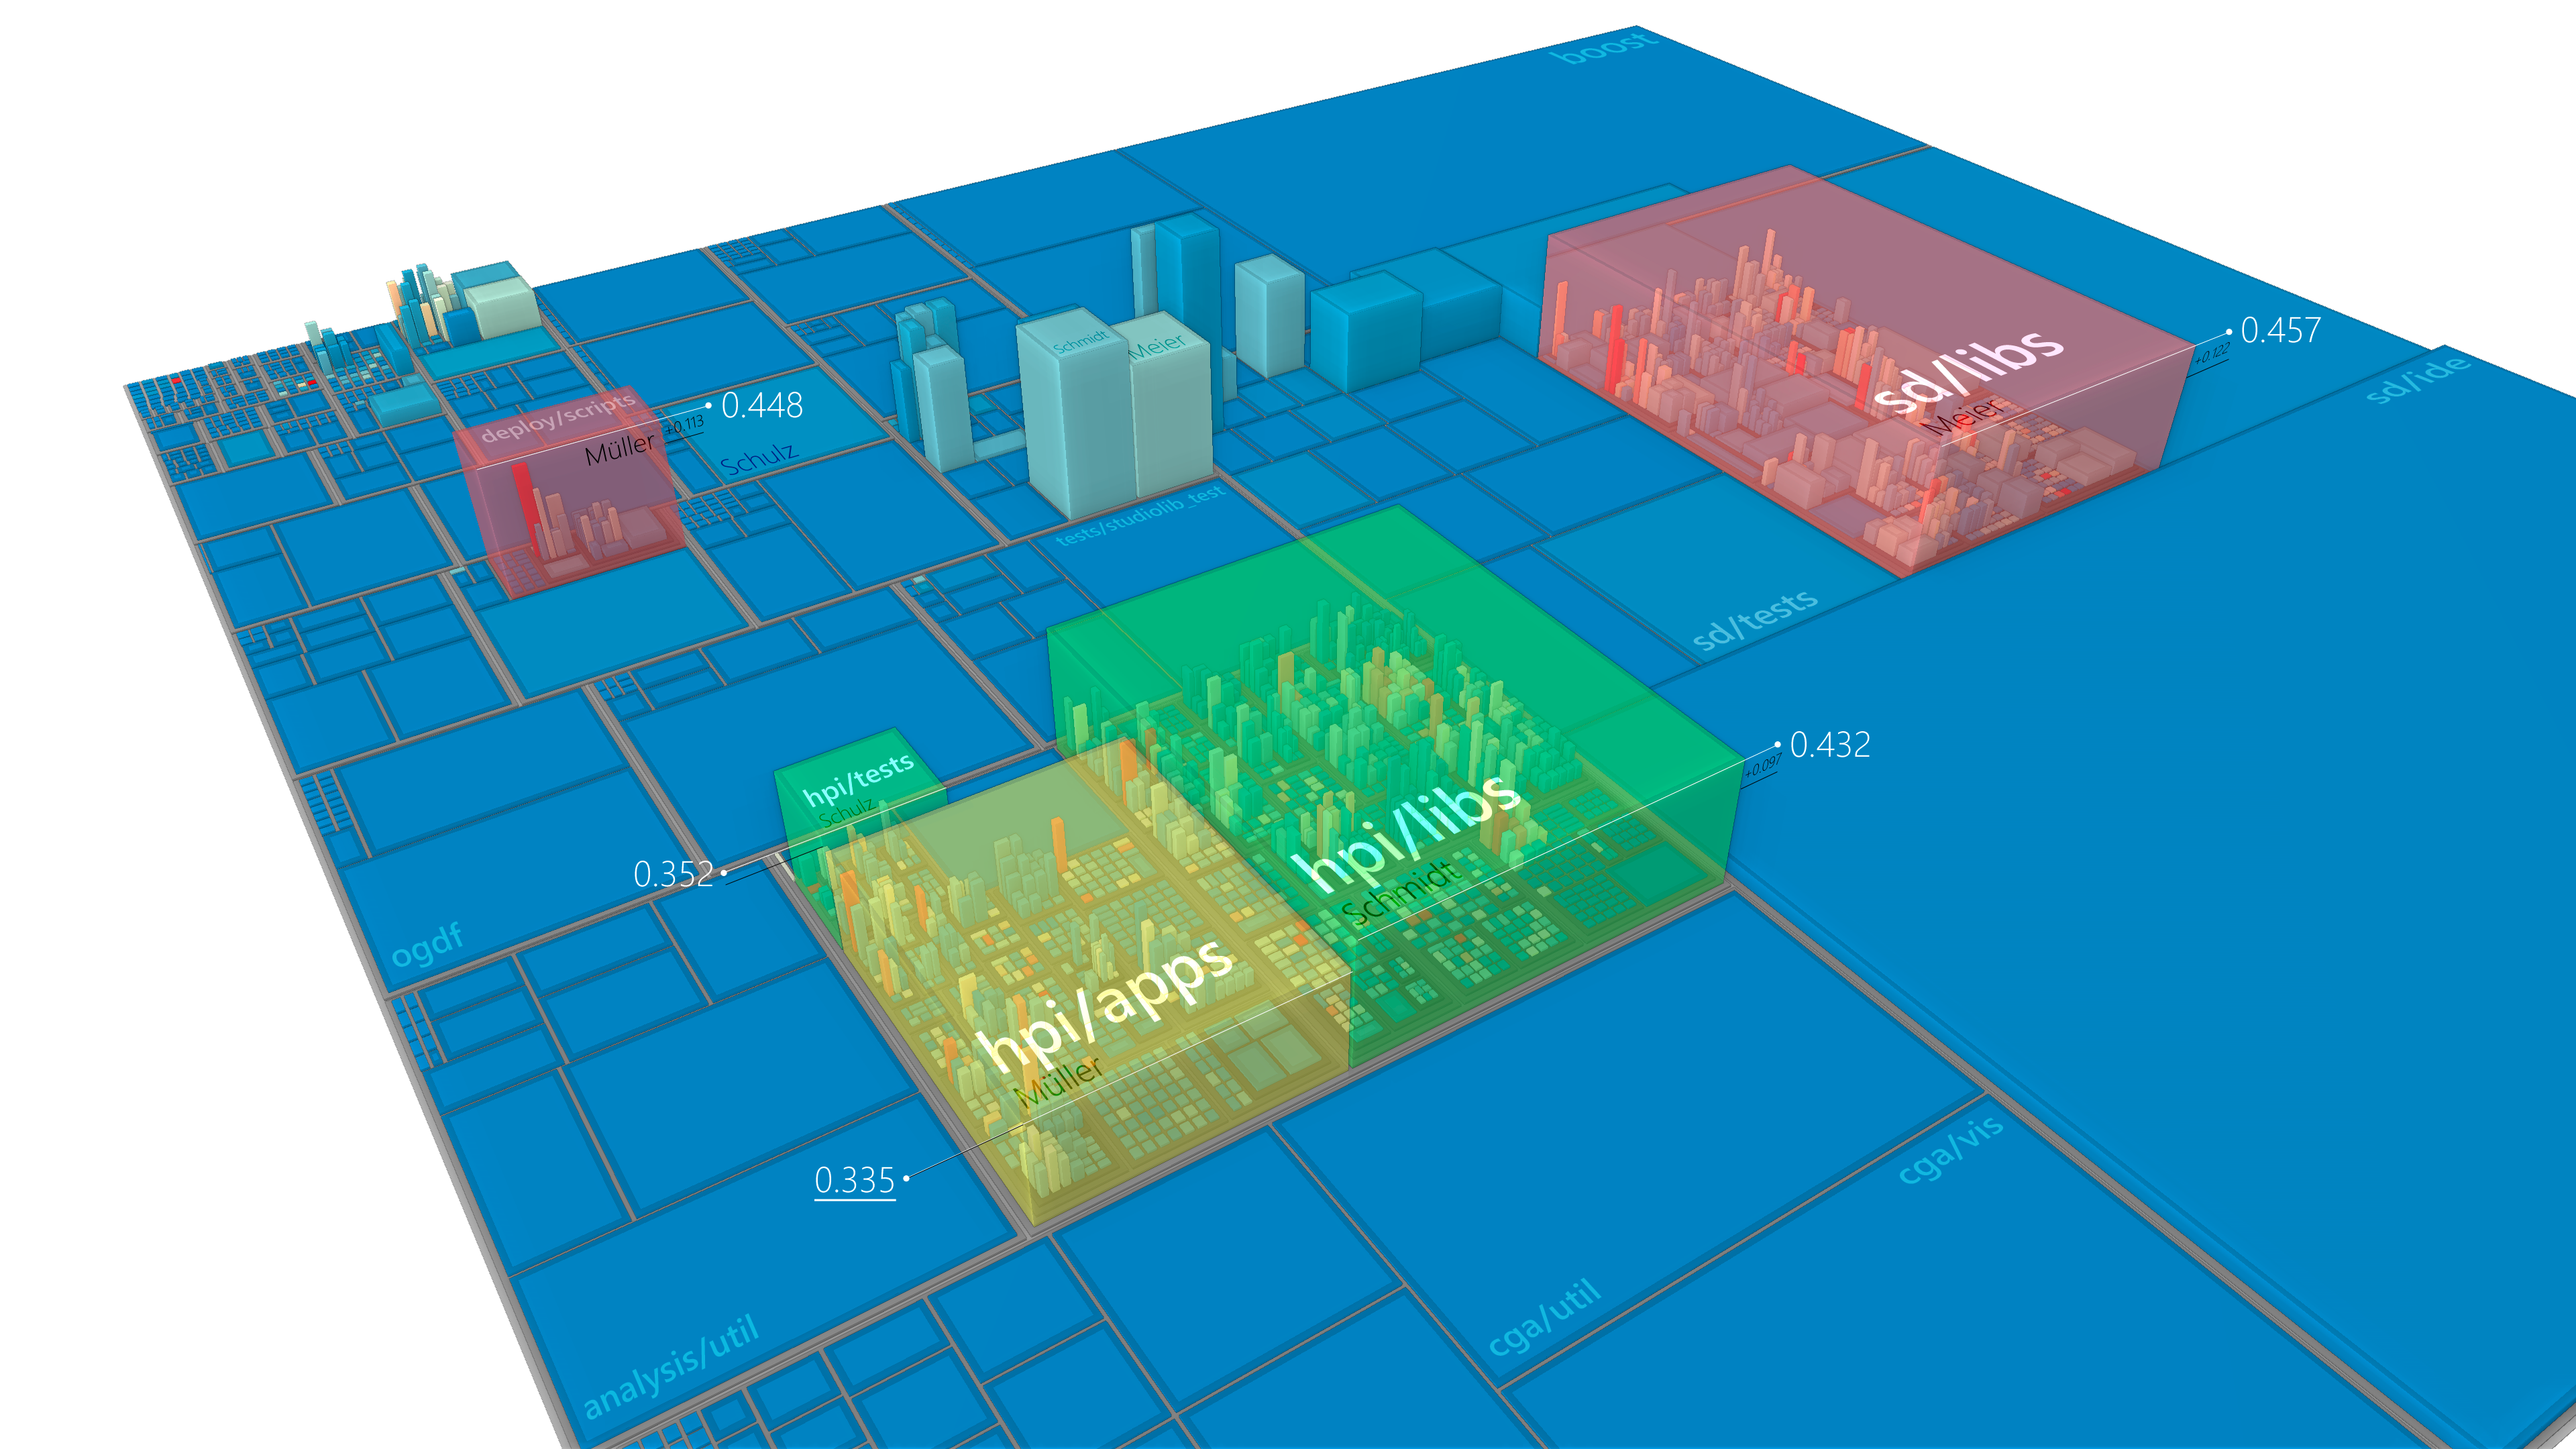
\includegraphics[height=\paperheight]{images/showcase/multi-semantic-treemap}}
\begin{frame}{~}
\end{frame}
}

\begin{frame}[c]{Oberservations}
      
    \centering 
    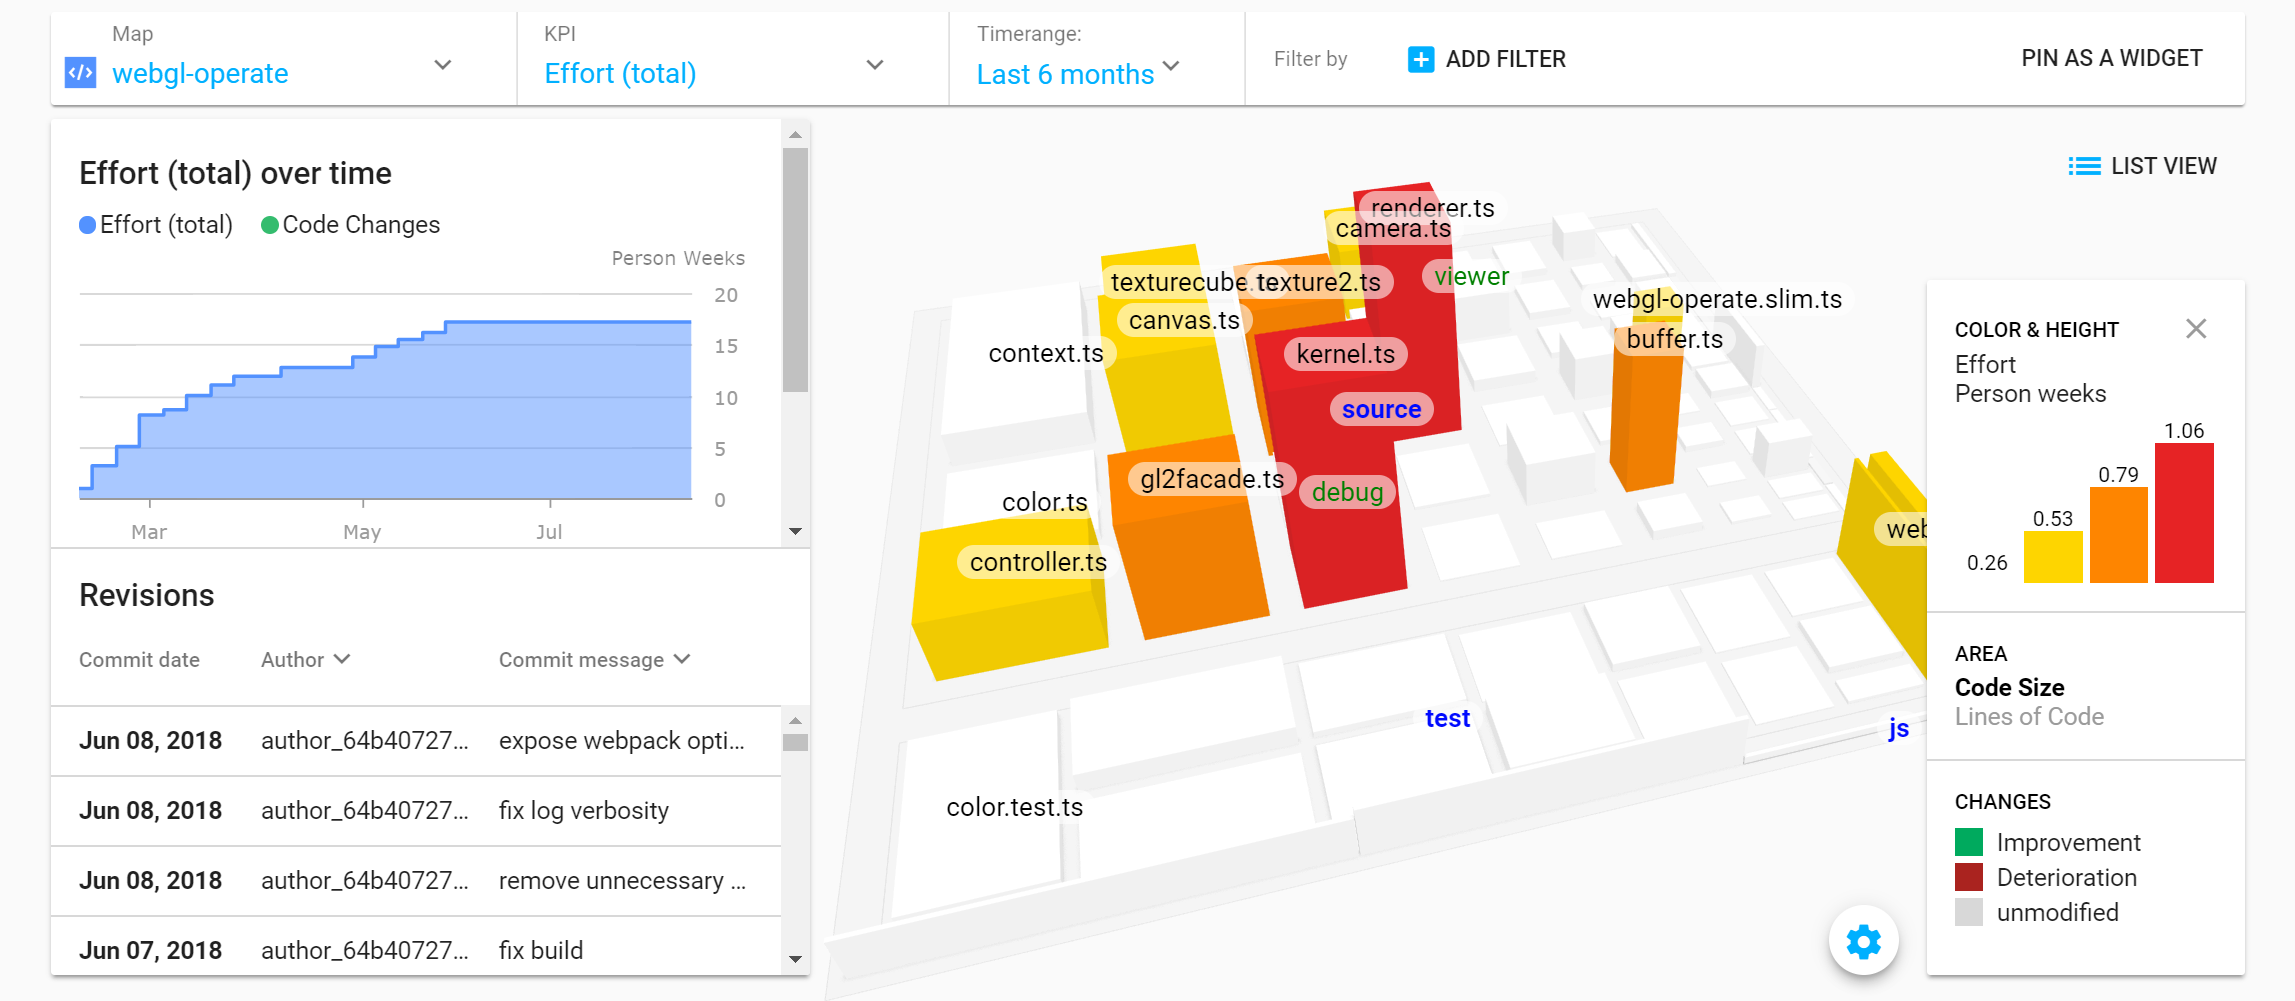
\includegraphics[height=0.65\paperheight]{images/platform}
    \medskip

    Height is often used merely as rough indication of data trends or color reinforcement.

\end{frame}

\begin{frame}[c]{Problem Statement}

    \begin{itemize}
        \item Capability of height-related queries for filtering and identification of nodes-of-interest is missing.
        \item User height estimates might be hindered due to perspective foreshortening, occlusion, or height-distorting inner node representations:
    \end{itemize}

    \centering
    \begin{columns}
    
         \begin{column}{0.27\textwidth}
            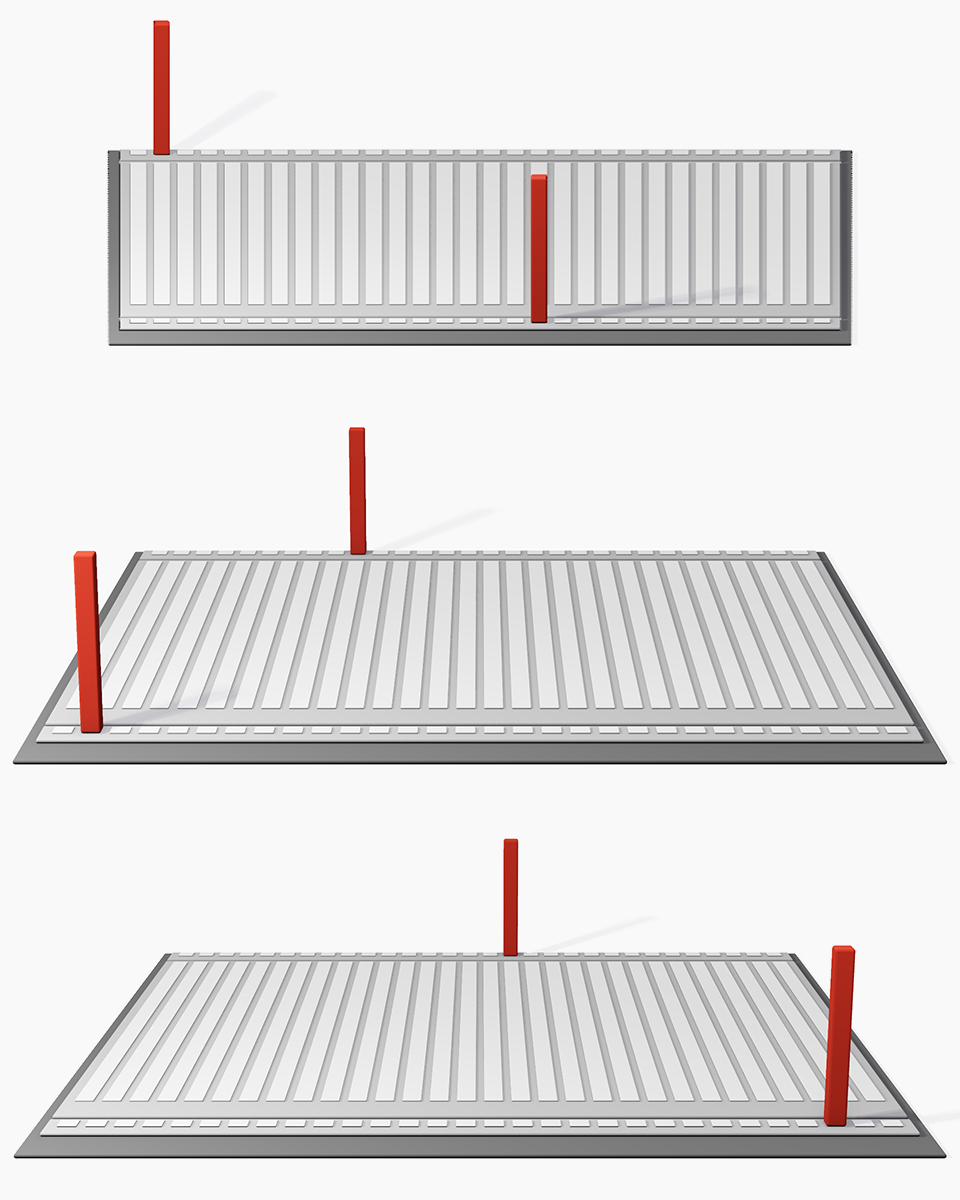
\includegraphics[width=\textwidth]{images/height-front-back}
         \end{column}

         \begin{column}{0.20\textwidth}
            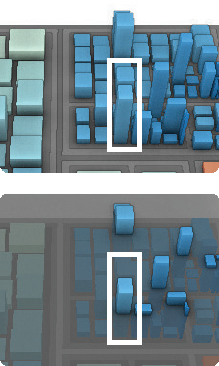
\includegraphics[width=\textwidth]{images/missleading-due-to-occlusion}
         \end{column}

         \begin{column}{0.24\textwidth}
            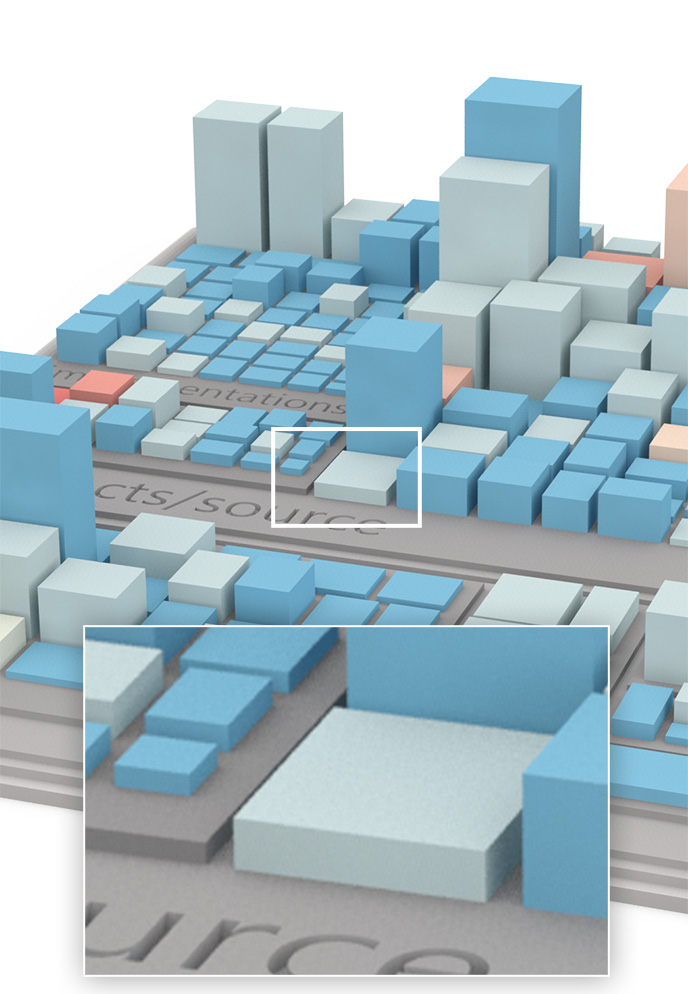
\includegraphics[width=\textwidth]{images/stacked-parents}
         \end{column}

    \end{columns}

\end{frame}

\begin{frame}[c]{Height Reference}

    Height reference denotes the visual display of an height threshold that can be interactively modified and used for height-based queries in 2.5D treemaps.
    \bigskip

    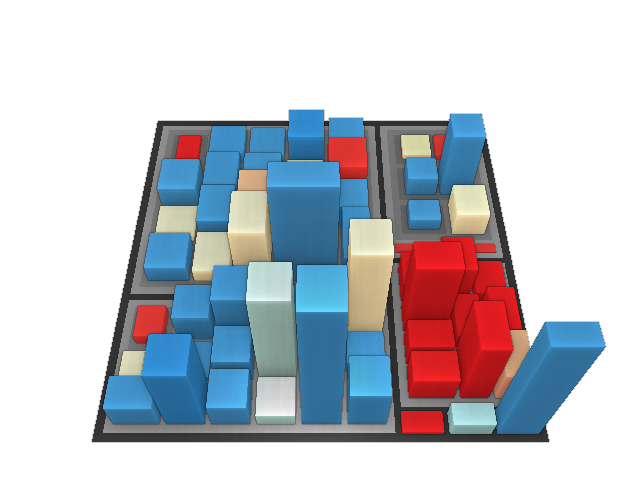
\includegraphics[width=0.084\textwidth]{images/glow-plain/1}
    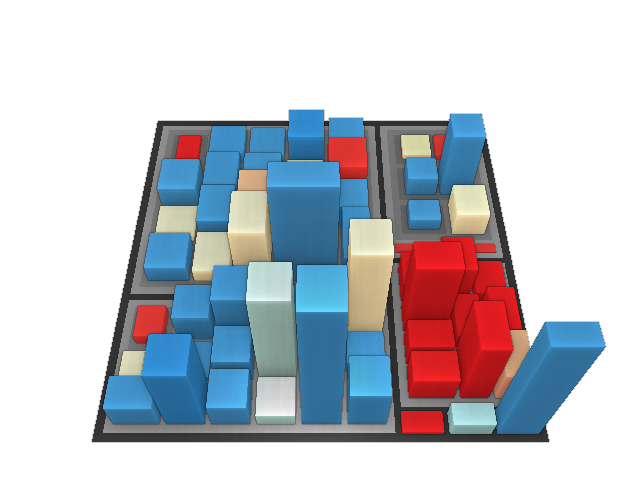
\includegraphics[width=0.084\textwidth]{images/glow-plain/2}
    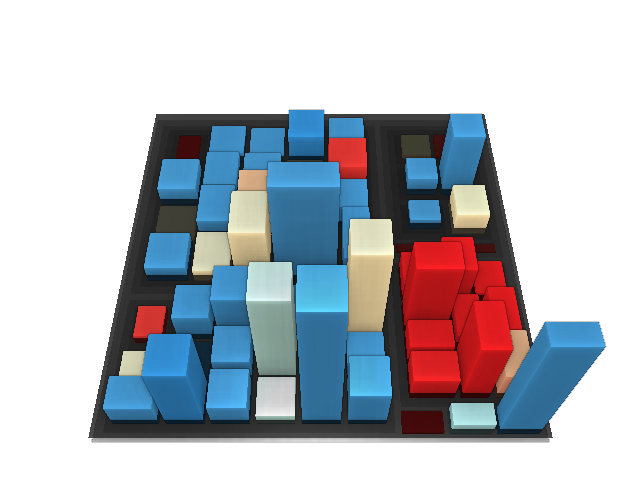
\includegraphics[width=0.084\textwidth]{images/glow-plain/3}
    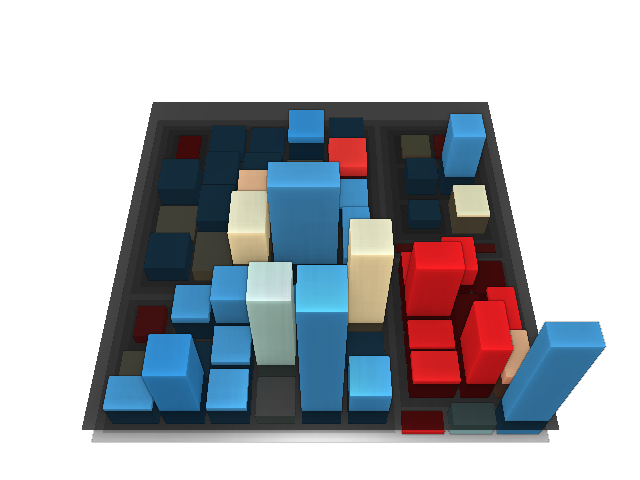
\includegraphics[width=0.084\textwidth]{images/glow-plain/4}
    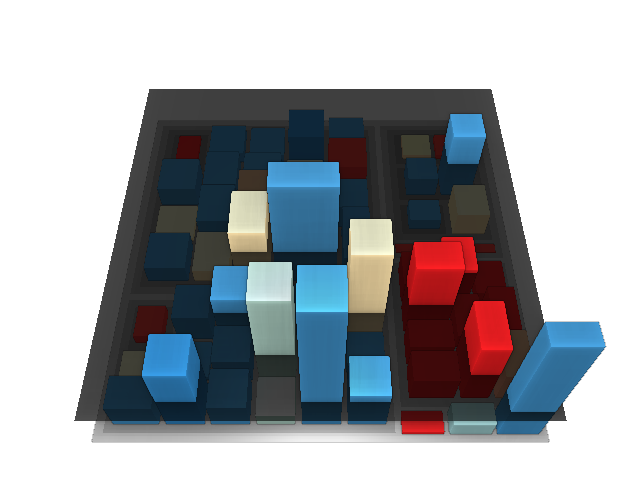
\includegraphics[width=0.084\textwidth]{images/glow-plain/5}
    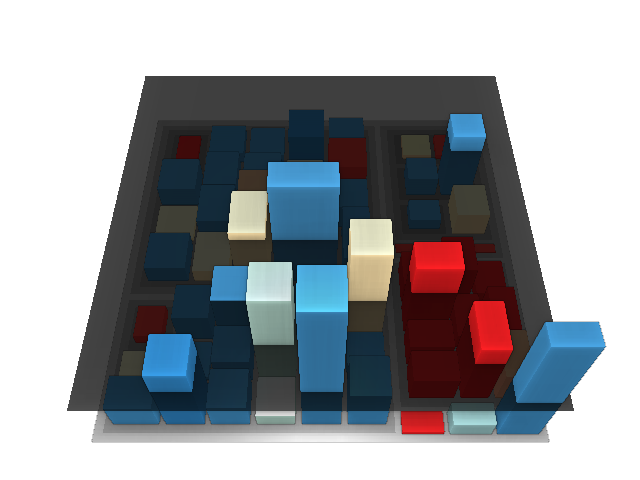
\includegraphics[width=0.084\textwidth]{images/glow-plain/6}
    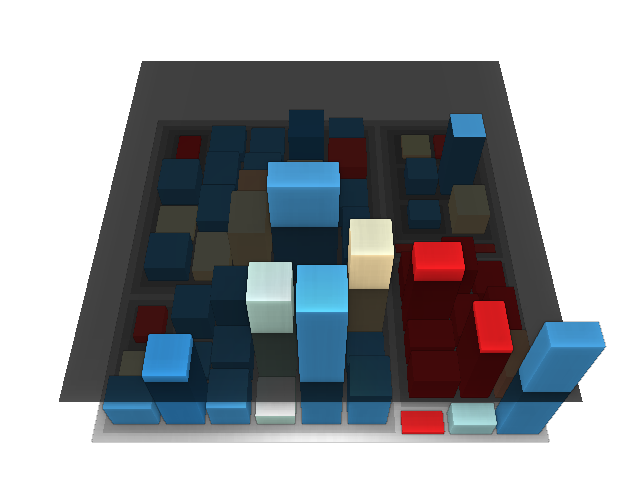
\includegraphics[width=0.084\textwidth]{images/glow-plain/7}
    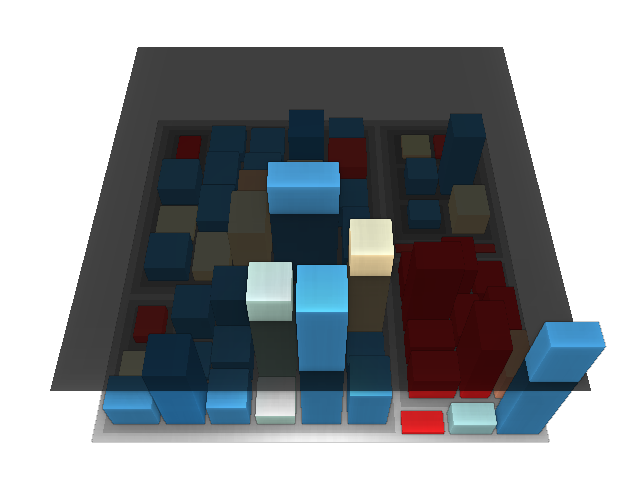
\includegraphics[width=0.084\textwidth]{images/glow-plain/8}
    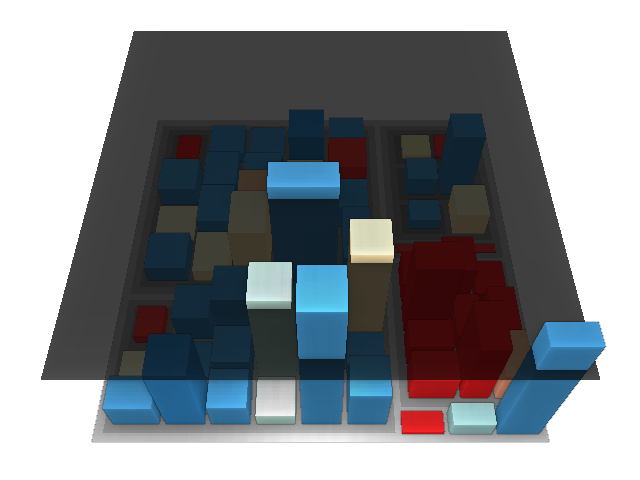
\includegraphics[width=0.084\textwidth]{images/glow-plain/9}
    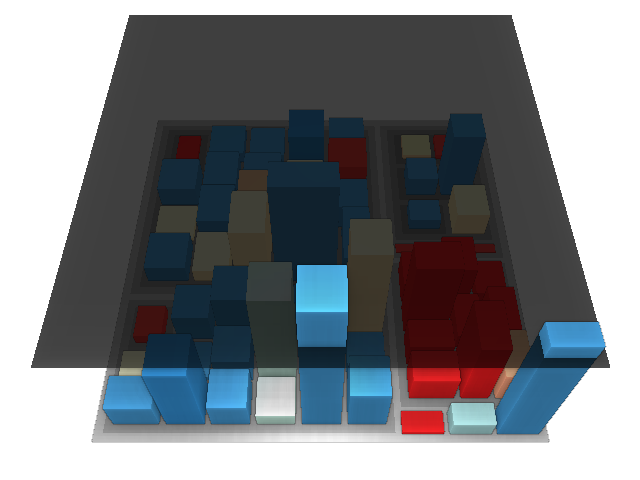
\includegraphics[width=0.084\textwidth]{images/glow-plain/10}
    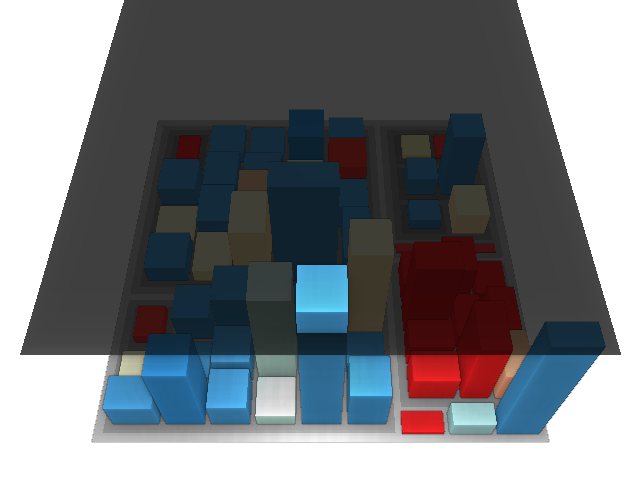
\includegraphics[width=0.084\textwidth]{images/glow-plain/11}
    \bigskip
    \bigskip

    \pause

    \blueify{Height-based queries}:
    \begin{itemize}
        \item Highest Nodes --- Communication of order for identification of $n$ top-most nodes.
        \item Similar Nodes --- Accentuation of nodes of similar or same height (peers).
        \item Thresholded Nodes --- Exclusion or inclusion of nodes below or above a threshold respectively.
    \end{itemize}

\end{frame}

\begin{frame}[c]{Visual Display --- Prerequisites}

    \begin{itemize}
        \item Simultaneous use of cuboids for leaf and inner nodes is avoided (or applied with care).
        \medskip

        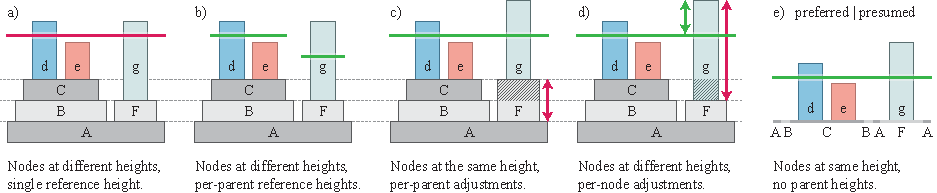
\includegraphics[width=0.96\textwidth]{images/parent-height-issues}
        \medskip

        \pause
        
        \item The mapping correlates cuboid height to relevance for any specific task.
        If small or negative values are relevant for a specific task, an inverted height mapping is expected (highest node).
        \medskip

        \item The height range is rather small to avoid occlusion and promote pre-attentive color processing.
    \end{itemize}
    
\end{frame}

\begin{frame}[c]{Visual Display --- Variations and Constraints}
    
    \bigskip

    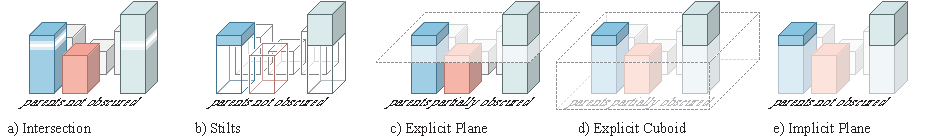
\includegraphics[width=\textwidth]{images/height-reference-variations}
    \medskip

    \begin{itemize}
        \item Should not rely on transparency or translucency (rendering complexity and cost).
        \item Should be orthogonal to other visual variables (e.g., transparency, procedural texturing, texturing).
        \item Should not obscure the visual display of inner nodes (e.g., labeling and/or coloring).
        \item Increasing the height threshold should reduce the overall visual complexity.
    \end{itemize}

\end{frame}

\begin{frame}[c]{Interaction --- Approach and Constaints}
    
    \medskip
    The height reference can be manipulated by either touching a cuboids lateral faces or its top, and thereby specifying the height threshold (y-coordinate at intersection with cuboid):
    \bigskip

    \begin{columns}
        \begin{column}{0.467\textwidth}
            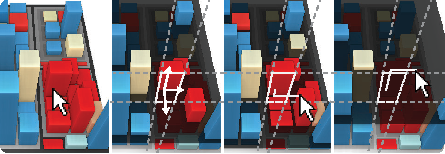
\includegraphics[width=\textwidth]{images/cuboid-height-interaction-lateral}\medskip

            \centering\small
            Interaction with Lateral Faces
        \end{column}

        \begin{column}{0.467\textwidth}
            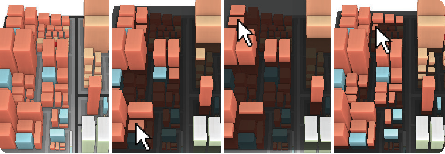
\includegraphics[width=\textwidth]{images/cuboid-height-interaction-top}\medskip

            \centering\small
            Interaction with Top Face
        \end{column}

    \end{columns}
    \bigskip
    \medskip

    \pause

    Constraint: 
    2.5D treemap most likely provides navigation (pan, zoom, rotate), as well as temporary emphasis (e.g., outlining), (un)folding and/or (de)selection of nodes already.
    Thus, height reference interaction should be exposed using a specific interaction mode (e.g., modifier key).

\end{frame}

\begin{frame}[c]{Preliminary User Study}
    
    $H_1$ \enspace Users can identify differences in node heights faster when using the height reference.\newline
    $H_2$ \enspace Users can identify nodes of specific heights more accurate when using the height reference.
    \bigskip

    \begin{columns}
        \begin{column}{0.467\textwidth}

            The study was conducted with 20 participants and the following preliminary results:
            \begin{itemize}
                \item $H_1$ (Speed) not confirmed: 
                The average time to response for each task was slightly faster without the use of the height reference.
                \item $H_2$ (Accuracy) confirmed: Using the height reference increased the accuracy
                by 25\% (similar nodes) to 42\% (top 3 nodes) over the task completed without height reference.
            \end{itemize}

        \end{column}

        \begin{column}{0.467\textwidth}
            \medskip
            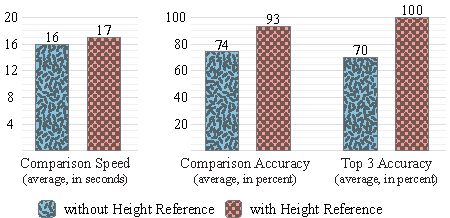
\includegraphics[width=\textwidth]{images/user-study-results}

        \end{column}

    \end{columns}

\end{frame}

\begin{frame}{Conclusion and Contact Information}

   \begin{columns}
        
        \begin{column}{0.28\textwidth}           
            
            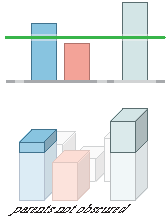
\includegraphics[width=\textwidth]{images/credits}
    
        \end{column}

       \begin{column}{0.6\textwidth}              
           
            This talk presented
           \begin{itemize}
                \item the concept of a \blueify{height reference},
                \item an approach for its \blueify{visual display}, and
                \item a respective basic \blueify{interaction model} 
           \end{itemize}        
           in order to facilitate height-based queries in 2.5D treemaps.

            \bigskip
            \bigskip 
        
            Author email addresses: 
            \begin{itemize}
                \item \blueify{\underline{daniel.limberger@hpi.de}}
                \item \blueify{matthias.trapp@hpi.de}
                \item \blueify{juergen-doellner@hpi.de}
            \end{itemize}
            \medskip

        \end{column}

    \end{columns}

\end{frame}

\begin{frame}[allowframebreaks]{Bibliography}
    \bibliographystyle{acm}
    \setbeamertemplate{bibliography item}{\insertbiblabel}
    \bibliography{references}
    \vfill
\end{frame}

\begin{frame}{Software Maps --- Map Theme}
    
    \begin{columns}
        
        \begin{column}{0.6\textwidth}
            \Large For a given task, a \blueify{map theme} specifies the\\mapping of attributes to visual variables.
        \end{column}   
        
        \begin{column}{0.34\textwidth}
            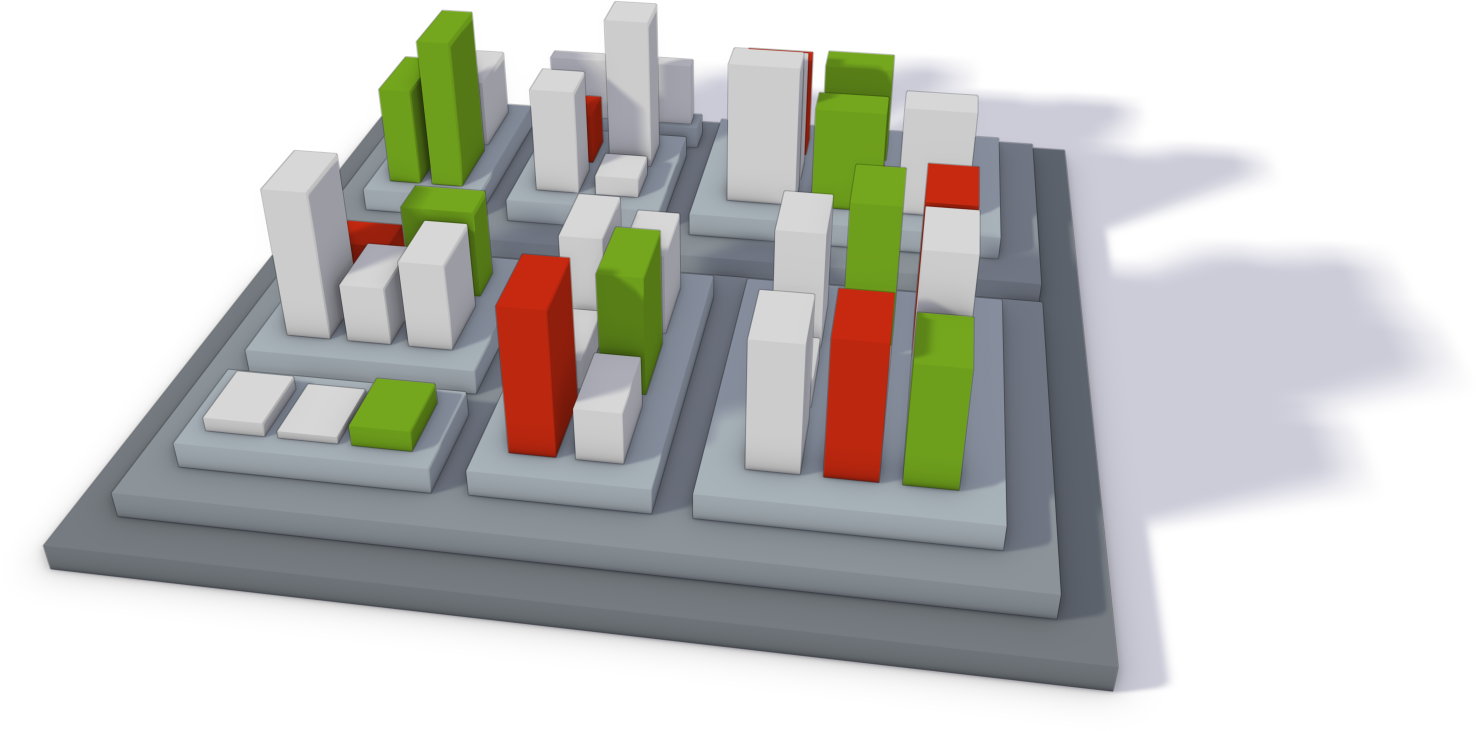
\includegraphics[width=2in]{images/app-maps}
        \end{column}   
        
    \end{columns} 
    
    \medskip
    \normalsize    
    
    \begin{description}
        
        \pause
        \item[\blueify{Technical Depth}] maps logic lines-of-code to weight, a nesting-level metric to color, and McCabe complexity \cite{McCabe1976}.
        It is used to reveal and monitor the 'technical debts' inherent to a software system's implementation.
        
        \pause
        \item[\blueify{Risk of Knowledge Drain}] maps logic lines-of-code to weight, the number of active developers to color, and a composite, nesting-level or McCabe based complexity measure indicating difficult-to-comprehend code to height. It is used to identify complex code units known only by few developers and reveal knowledge distribution.        
        
    \end{description}
    
\end{frame}

\begin{frame}[t]{Software Maps --- Goals}
    
    \bigskip
    
    \begin{columns}
        
        \begin{column}{0.65\textwidth}
            
            Make code quality of software systems visible to \enquote{stakeholders in the development process, particularly, to the management} \cite{Bohnet2011} by means of depicting, e.g., metrics and activity data.
            
            \bigskip
            \blueify{Depending on the applied map theme Software Maps facilitate}
            \begin{itemize}
                \item exploring structures,
                \item monitoring development processes,
                \item monitoring software quality, and
                \item identifying areas that require attention in the ongoing development process.
            \end{itemize}
            
        \end{column}   
        
        \begin{column}{0.28\textwidth}
            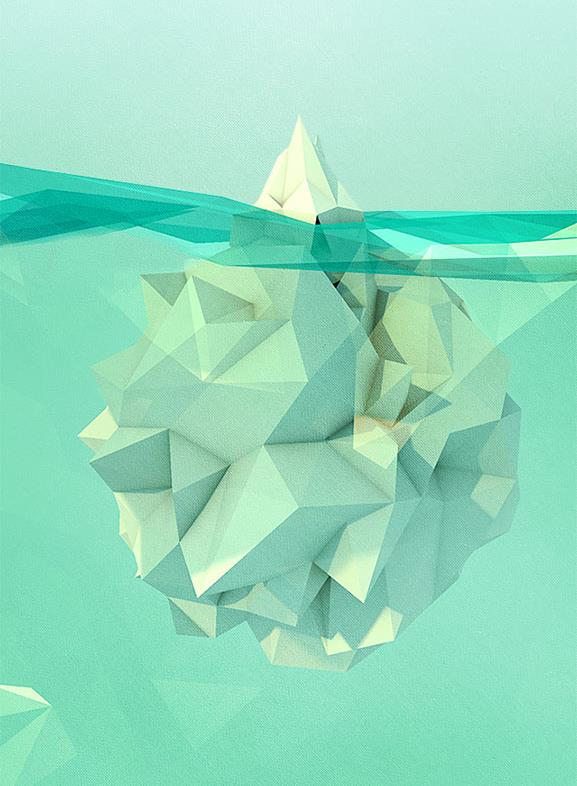
\includegraphics[width=1.5in]{images/iceberg}        
        \end{column}   
        
    \end{columns}
    
\end{frame}

\end{document}

